% --------------------------------------------

% AP: I have some compatibility issues with the new style (i.e. \section does not work)
\IfFileExists{emulateapjlegacy.cls}{\documentclass[iop]{emulateapjlegacy}}{\documentclass[iop]{emulateapj}}

\usepackage{amsmath}
preamble.tex
\slugcomment{To be Submitted.}

\makeatletter
\renewcommand\normalsize{\@setfontsize\normalsize\@xpt{12.5}}
% \renewcommand\normalsize{\@setfontsize\normalsize{10.56}{11.4}}      % 11.5, 12.5
\makeatother

\usepackage{xcolor}
\definecolor{apcolor}{HTML}{b3003b}
\definecolor{dlcolor}{HTML}{FF7F00}
\newcommand{\AP}[1]{({\bf \color{apcolor} AP: #1})}
\newcommand{\DL}[1]{({\bf \color{dlcolor} DL: #1})}

\citestyle{aa}
\shorttitle{Dynamical Properties of Molecular Cloud Complexes in Galaxies at the Epoch of Reionization
}
\shortauthors{Leung et al.}

\begin{document}
\title{
Dynamical Properties of Molecular Cloud Complexes in Galaxies at the Epoch of Reionization
}


\author{T. K. Daisy Leung\altaffilmark{1, 2}}
\author{Andrea Pallottini\altaffilmark{3, 4}}
\author{Andrea Ferrara\altaffilmark{4, 5}}
\author{Mordecai-Mark Mac Low\altaffilmark{2, 6, 7}}

\affil{\textsuperscript{1} Department of Astronomy, Space Sciences Building, Cornell University, Ithaca, NY 14853, USA; }
\email{tleung@astro.cornell.edu}
\altaffiltext{2}{Center for Computational Astrophysics, Flatiron Institute, 162 Fifth Avenue, New York, NY 10010, USA}
\altaffiltext{3}{Centro Fermi, Museo Storico della Fisica e Centro Studi e Ricerche ``Enrico Fermi'', Piazza del Viminale 1, Roma, 00184, Italy}
\altaffiltext{4}{Scuola Normale Superiore, Piazza dei Cavalieri 7, I-56126 Pisa, Italy}
\altaffiltext{5}{Kavli Institute for the Physics and Mathematics of the Universe (IPMU), The University of Tokyo, 5-1-5 Kashiwanoha, Kashiwa 277-8583, Japan}
\altaffiltext{6}{Institut f{\"u}r Theoretische Astrophysik, Zentrum f{\"u}r Astronomie der Universit{\"a}t Heidelberg, 69120 Heidelberg, Germany}
\altaffiltext{7}{American Museum of Natural History, 79th St.~at Central Park West, New York, NY 10024, USA}


\begin{abstract}
We study the dynamical properties of molecular clouds complexes (MC) in a prototypical galaxy (\flower)
and its satellite galaxies at the Epoch of Reionization (EoR) using cosmological zoom-in simulation.
We identify MCs using H$_2$ density, 
and compare their masses, sizes, velocity dispersions, gas surface densities, and virial parameters ($\alpha_{\rm vir}$)
with those observed in nearby and \z$\sim$\,2 galaxies.
The MCs span a mass range of $10^{6.5-9}$\,\Msun. Their velocity dispersions and gas surface densities are 
systematically higher than those observed in nearby galaxies, but comparable to starburst galaxies.
We compute the effective two-component Toomre $Q$ parameter (gas and stars) to examine 
regions that are unstable to local axisymmetric perturbations. 
We further perform virial analysis, which is accessible from observations, to examine regions likely 
to undergo collapse.
Our analysis indicates that the MCs in the main disk of \flower are unbound, but its 
substructures have lower virial parameters, which is
consistent with the notion that collapsing structures result from gravitational instability within globally stable structures.
% , which are supported by turbulence and rotation on large scale.
On the other hand, we find $\alpha_{\rm vir}\approx$\,2 for the MCs in the satellite galaxies,
which we interpret as result of the weaker stellar feedback and less frequent \SF compared to \flower.
Our results suggest that the more massive and bigger MCs compared to the Milky Way
manifest from the higher gas mass fraction, surface density, and velocity dispersion.
% , which together sets the scale for fragmentation.
High resolution imaging of the first galaxies with the Atacama Large (sub-)Millimeter Array (ALMA) and the
Next Generation Very Large Array (ngVLA)
can furnish scrutinizing data to test our findings and shed light on \SF since the cosmic dark ages.
\end{abstract}
\keywords{methods: data analysis --
          galaxies: high-redshift --
          galaxies: ISM --
          galaxies: evolution --
          galaxies: formation --
          galaxies: starburst --
          stars: formation}

% it can be instead included as
% \graphicspath{{Fig/}}
% so that plots are automatically searched for in the given path
\def\figpath{./Fig}

%--------------------------------------------------------------------------
%                                Introduction
%--------------------------------------------------------------------------
\section{Introduction}    \label{sec:intro}

The growth of galaxies and their subsequent evolution are governed by the baryon cycle ---
galaxies accrete gas from the intergalactic medium (IGM) to fuel \SF (and feed their supermassive blackholes)
and subsequent feedback replenishes and enriches the circumgalactic medium with part of this material.
The general consensus is that the growth of \highz galaxies are triggered and supported by massive
gas inflows from mergers and/or the cosmic web at early cosmic time, when the IGM and galaxies themselves
are more gas-rich in their star-forming molecular
gas contents compared to present-day galaxies.
% while at a given snapshot, the gas mass fraction maybe low (esp. at high-z when
% the gravitational potential is still increasing), but their gas reservoirs
% are continuously being replenished.
These massive gas inflows in turn trigger gravitational instability and lead
to the formation of gas structures that are typically more massive and denser than those
observed in nearby galaxies, with masses of $M_{\rm cl}$\eq10$^9$\,\Msun
and sizes on sub-kpc scales (e.g., \citealt{Gabor13a, Hopkins14a, Inoue16a}).
Some theoretical works argue that the
migration of such giant massive clumps are responsible for contributing to the
buildup of the bulges of massive galaxies at \z$\sim$\,0 \citep[e.g.,][]{Ceverino10a}.

Given that \highz galaxies are the early stages of evolution of present-day galaxies, studying their ISM properties is essential for understanding how \SF proceed under these relatively more extreme conditions, thereby driving the evolution and assembly
of galaxies
since the cosmic dark ages.
Current consensus is that at higher redshifts, galaxies have higher
star formation rates \citep[SFR; ][]{Behroozi13b, Sparre15a, Maiolino15a, Dunlop17a} and
smaller sizes \citep[e.g.,][]{Bouwens11a, Ono13a} compared to those found in the local Universe.
The former are thus expected to have more \ion{H}{2} regions, ionized gas, and more intense radiation stellar feedbacks.
Since their metallicity and dust content are also expected to be lower as they are assembling,
this affects the shielding of UV photons, heating and cooling mechanisms in these early systems. Such differences in turn
affect the regulation of thermal and chemical structures of their ISM.
Their multi-phase ISM and the dynamics of the star-forming molecular cloud complexes (MC)
are therefore expected to differ from nearby galaxies.
Even in the local Universe, where the most detailed \obs can be attained, variations in cloud properties have been
observed between different galaxy populations (see e.g., \citealt{Hughes10a, Hughes13b}).
It is thus intuitive and reasonable to pose the question: what are the dynamical states of the MCs of the first galaxies and
how do they differ from the local Universe, and are they analogous to any seen in the local \galpop?
%

The FIR fine-structure lines (e.g., \cii, \nii, and \oiii), and CO and [\ci]~lines are the key diagnostics for
constraining the ISM conditions of a galaxy by
providing highly complementary information that trace different phases of the ISM (ionized,
atomic, molecular; e.g., \citealt{Scoville74a, Rubin85a, Malhotra01a}).
Global measurements of these diagnostics in \highz galaxies
have informed us on their galaxy-wide properties (e.g.,
gas masses, gas temperature, and radiation field intensity).
However, spatially resolving their ISM is necessary to understand their roles in galaxy evolution and
the physics behind their intense \SF (SFR\ssim100$-$3000\,\Msun\,yr\pmOne).
To date, spatially resolved ISM properties of \highz galaxies
have only been examine observationally in a handful of (strongly-lensed)
galaxies, using tracers such as
dust continuum, CO, and \cii lines (e.g., \citealt{Swinbank11a, Hodge15a, Ferkinhoff15a, Hodge16a, Leung19a}).
These studies find that galaxies at $z$\ssim2 galaxies, close to the peak of cosmic \SF, are more
molecular gas-rich, turbulent, and clumpy than nearby galaxies.
That said, it remains unclear how \SF proceed in the (sub-)$L^*$ galaxy population at \z$\gtrsim$\,6 ---
the epoch of reionization  ---
which is responsible for producing the
ionizing photons that reionized the Universe.
While ALMA has enabled the detections of
ISM diagnostic lines e.g., the \cii158\,$\micron$ and CO line emission in
normal (SFR$<$\,100\,\Msun\,yr\pmOne) galaxies at \z$>$\,6 over the past few years \citep[e.g.,][]{Odorico18a, Carniani18b},
we are still far from mapping their molecular ISM due to the cosmological dimming.
As such, we have undertaken a study, exploiting
state-of-the-art cosmological zoom-in hydrodynamic simulation
\ncode{Serra} (Greenhouse in Italian; \citealt{Pallottini17a, Pallottini17b}), with a goal to examine
and predict the dynamical properties of the star-forming molecular cloud complexes in a \z$\sim$6 prototypical (i.e., $L^*$)
galaxy. % to understand the physics behind \SF in the first galaxies.

This paper is structured as follows.
In \Sec{sim}, we describe the setup of our simulation and properties of our main galaxy (\flower),
and describe the method used to identify its molecular gas complexes.
In \Sec{eqn}, we present the formalism within which we interpret the results.
In \Sec{results}, we present scaling relations for the MCs identified. 
% Toomre stability analysis in \Sec{Q}.
We then interpret the results   % , robustness of our analysis, caveats,
and discuss the implications of our findings in \Sec{diss},
and present our conclusions in \Sec{conclusion}.
Throughout this paper, we adopt a concordance cosmology, with total matter, vacuum and baryonic densities
in units of the critical density $\Omega_{\Lambda}$\eq0.692, $\Omega_m$\eq0.308, $\Omega_b$\eq0.0481,
Hubble constant $H_0$\eq100\,$h$\,km s\pmOne\,Mpc\pmOne with $h$\eq0.678,
spectral index $n$\eq0.967 and $\sigma_8$\eq0.826 \citep{Planck14a}.


% ------------------
\section{Simulation and Method} \label{sec:sim}


\subsection{\ncode{Serra} Simulation\footnote{Serra means greenhouse in Italian which is motivated by the
fact that our simulation includes a chemical network to calculate the abundance of H$_2$, which in turn
dictates the formation of CO.
}}
The simulation used in this work is described by \citealt{Pallottini17a, Pallottini17b} and is briefly summarized here.

\ncode{Serra} is a suite of cosmological zoom-in simulations performed using Eulerian hydrodynamics and
adaptive mesh refinement (AMR) technique to achieve high spatial resolution in the region of interest (i.e., regions of high density).
In particular, it uses a modified version of \ncode{ramses} \citep{Teyssier2002a} as the AMR backend.
Our simulation covers a co-moving box of 20\,Mpc $h$\pmOne in size, resolving down to a physical scale of $l\approx$\,30\,pc (at \z$\sim$\,6) and a (baryonic) mass resolution of $m_b\simeq$\,10$^4$\,\Msun at the finest level. Such a physical scale is close to the size scale of molecular cloud complexes and giant molecular clouds (GMCs) seen in nearby galaxies \citep[e.g.,][]{Sanders85a, Federrath13a, Goodman14a}.
We include chemical network in the simulation to trace $\rm{H}$, $\rm{H}^{+}$, $\rm{H}^{-}$, $\rm{He}$, $\rm{He}^{+}$, $\rm{He}^{++}$, $\rm{H}_2$, $\rm{H}_2^{+}$ \citep{Grassi14a,Bovino16a}.
Of particular importance to our study here is that our simulation includes non-equilibrium formation of molecular hydrogen (done on-the-fly) to determine the H$_2$ abundance (see \citealt{Pallottini17b} for effects of chemistry affected by non-equilibrium versus equilibrium H$_2$ formation).

% radiative feedback --> NT pressure
Star formation is modeled using a H$_2$-based prescription of the Schmidt-Kennicutt relation \citep{Krumholz09a}. We adopt stellar tracks from \ncode{starburst99} and include stellar feedback from supernovae and OB/AGB stars to account for energy dissipations. To couple the feedback to the gas, we employ sub-grid modeling for blastwaves, e.g., to account for the potential lost of energy inside the cell during a supernova explosion. The energy dissipated is then injected into the ISM in the form of kinetic and thermal energies. Radiation pressure on the dust and gas is also included (see \citealt{Pallottini17a} for details).

Details on the properties of \flower\ --- the main galaxy in our simulation --- are discussed in \citet{Pallottini17b}.
Briefly, by \z$\sim$6, \flower is a Lyman-break galaxy (LBG), hosted in a dark matter halo of mass $M_{\rm DM}\simeq$\,10$^{10}$\,\Msun at the center of a cosmic web knot, and accretes mass from the IGM mainly via three filaments of length $\simeq$\,100\,kpc. At \z$\sim$6, \flower has a stellar mass of $M_*\simeq$\,3\E{10}\,\Msun, a metallicity of $Z\simeq$\,0.5\,$Z_{\odot}$, a molecular gas mass of $M_{\rm H2}\simeq$\,5\E{7}\,\Msun, and a globally-integrated SFR of $\simeq$\,100\,\Msun\,yr\pmOne. It is therefore a prototypical galaxy at \z$\sim$\,6.

The simulation data contain information such as the density ($\rho$) and velocity ($v_x$, $v_y$, and $v_z$) fields, from which we calculate
the physical properties of each MC, such as mass and velocity dispersion.
Due to the nature of our AMR simulation, we regrid the simulation data into uniform grids for the analysis presented in this paper.
The grid size is defined
based on the highest resolution of the simulation data (i.e., the less refined regions are supersampled in the resulting uniform grids).



\subsection{Star Formation History} \label{sec:sfh}
One of the main advantages for studying the dynamical properties of molecular structures at
$z$\ssim6 in simulation is the fact that we can examine how their properties evolve
as a function of time.
This is advantageous especially at early cosmic epochs,
when the densest structures are beginning to form;
gas is constantly being accreted onto the central galaxy from the cosmic web and
satellite galaxies, thereby leading to bursts of \SF.
Meanwhile, tidal forces resulting from interactions with these surrounding
galaxies can disrupt the main disk and arms, likely leading to different dynamical states
for the molecular structures compared to more evolved galaxies found at
a later cosmic time (e.g., some molecular structures may disperse while others may agglomerate into more massive
ones). % mainly expecting differences in alpha_vir, sigma, M_cl.

\begin{figure*}[!htbp]
\centering
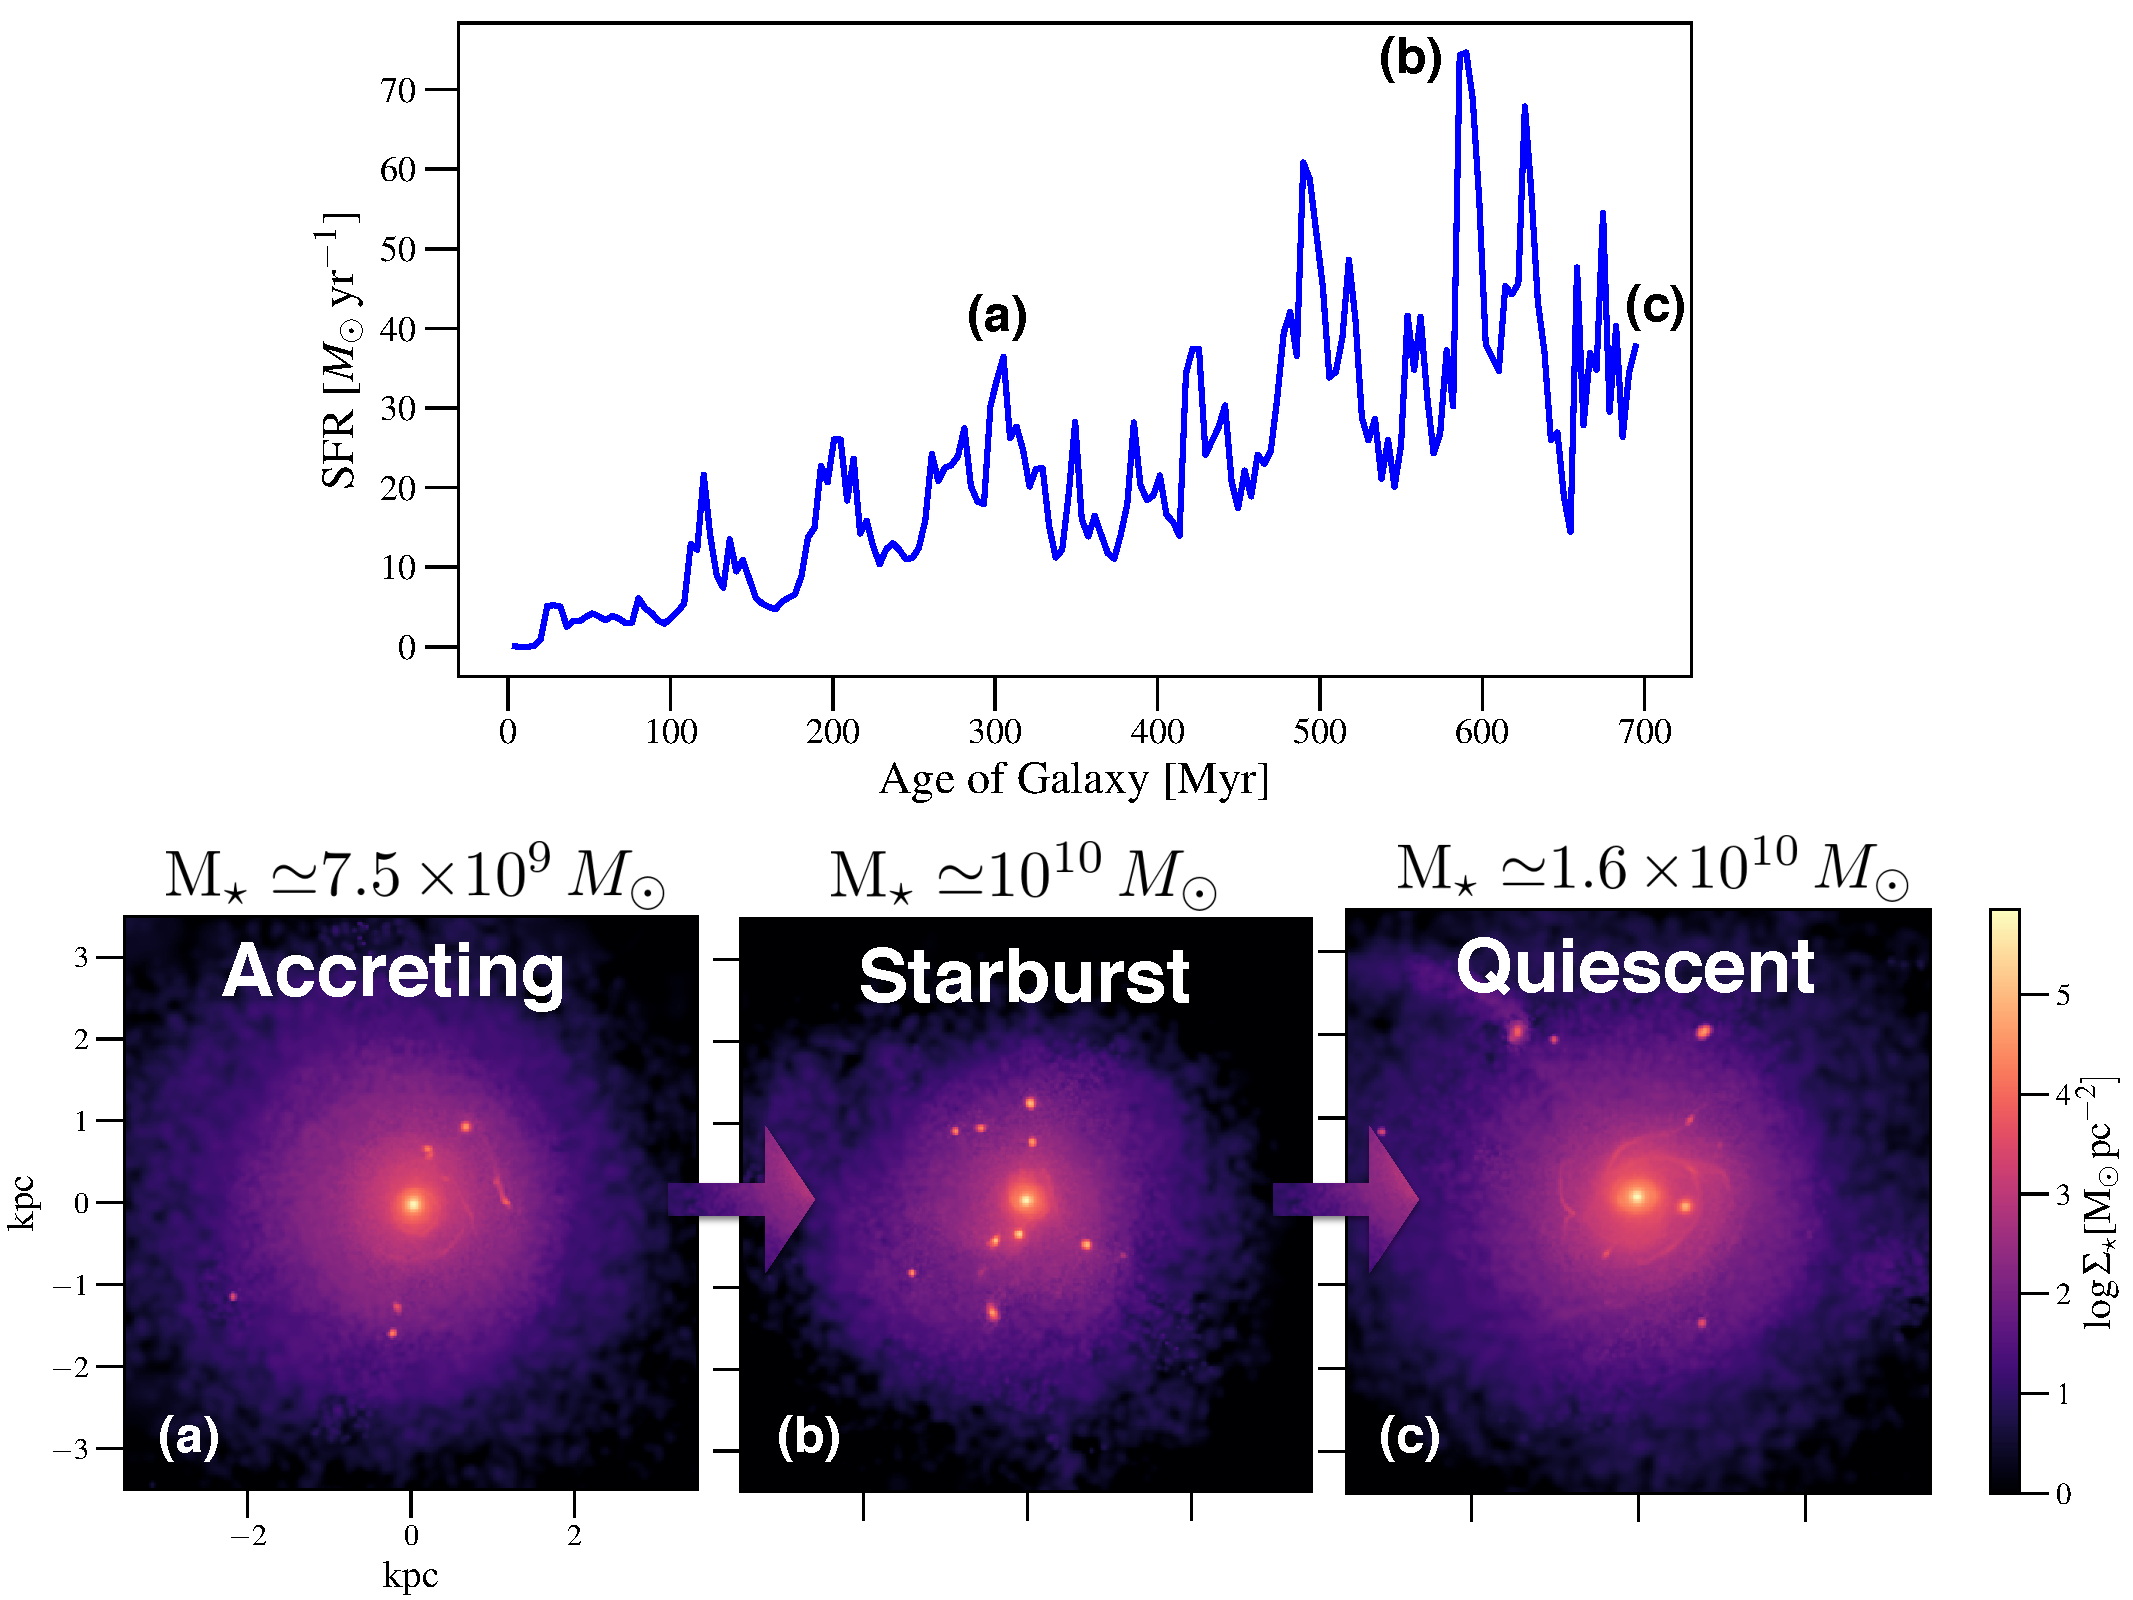
\includegraphics[trim=10 0 0 0, clip, width=0.65\textwidth]{\figpath/sfh.pdf}
\caption{
    Star formation history of \flower (top right) and
    projected stellar mass distribution of \flower during 
    {\it (a)} one of its accretion phases
    at its early stage of evolution; 
    {\it (b)} one of its major starburst phases
    after a major merger; and
    {\it (c)} a relatively quiescent phase post-starburst.
% f_gas history?
\label{fig:SFH}}
\end{figure*}


We show the \SF history of \flower in \Fig{SFH},
where the SFR is calculated based on existing young stellar population, which is
defined to have an age of $t_{\rm age}<$\,10\,Myr.
The SFR of \flower varies between $\sim$30$-$80\,\Msun\,yr\pmOne\footnote{
The SFR plotted in Figure 2 of \citet{Pallottini17b}
is a factor of two higher than shown here since they also include contributions from
massive satellite galaxies within the surrounding $\approx$50\,kpc, which
are accreted onto \flower at \z$\lesssim$\,2.}
as it evolves from an actively accreting phase to
a starburst phase after a major merger, and then back to a relatively quiescent phase,
over the few hundred Myr simulated in the simulation.

Given the stochasticity in the \SF history of \flower (see \Fig{SFH}),
we show the scaling relations found for two snapshots, corresponding to two of its most extreme evolutionary stages,
in \Sec{singless} to illustrate the salient points of the discussion presented in this paper.
The two phases (when \flower is accreting materials from its surrounding 
and when \flower is undergoing a major starburst phase) are expected to bracket the most extreme variations in the cloud dynamics. 


\subsection{Structure identification} \label{sec:method}
To identify the molecular complexes, we use a customized version of the clump-finding algorithm available in the \ncode{python} package \ncode{yt} \citep{Turk2011a}, which was initially described in \citet{Smith09a}, but this function has been modified since then.
%
The latest version of the default \ncode{yt} clump finder decomposes the zones in the simulation into non-overlapping tiles, which are stored in a k-dimensional tree (k-d tree). It then identifies the contours of a variable field (here, the density field) within a tile and connects them across the tiles.
In the customized version used for this study, we modify the function to enhance the stability of the code.
% (which essentially means we fixed the bugs in order for it to actually work).

In the ``clump-finding'' process, we employ a set of different density thresholds defined based on the
molecular hydrogen density of \flower taken at different cosmic times (between $z$\eq6.0\,$-$\,7.2).
We note that this process is in essence similar to
identifying molecular structures based on the noise levels of surface density maps
observers obtain with telescopes, using molecular line tracers such as CO, CS, and HCN,
as commonly adopted in observational studies (e.g., identifying
``clumps'' based on/after applying $\sigma$-clipping,
using tools such as \ncode{aips}'s task \ncode{serch}, \ncode{clumpfind},
and \ncode{cprops}; \citealt{Williams94a, Oka01a, Rosolowsky06a, Rosolowsky08a}).
We note that, owing to the nature of \obs, such structures are identified
in position-position-velocity (PPV) space, whereas in simulations, one has the
full 6D spatial-kinematic information, and can therefore cleanly identify structures directly using the density field in position-position-position (PPP) space.
% Many concerning the correspondence between  ... , dating back to the work by \citep{Adler92a}.
Existing studies find a good correspondence in the dynamical properties extracted in
PPV- versus PPP-space (\citealt{Ballesteros-Paredes02a, Heitsch09a, Shetty10a, Beaumont13a,
Pan15a}, but see also \citealt{Shetty10a} for a discussion on caveats and limitations).
% large scale structure in PPP may be identified as numerous lower mass structures in the PPV cube due to gradients in the LOS and conversly, superposition when spatially distinct components with the same velocity are "merged" into one component in the PPV space when observed along the LOS (see Fig. 1 of Beaumount13a). (may be worth putting more thoughts on this after the report is due).


\begin{figure}[htbp]
\centering
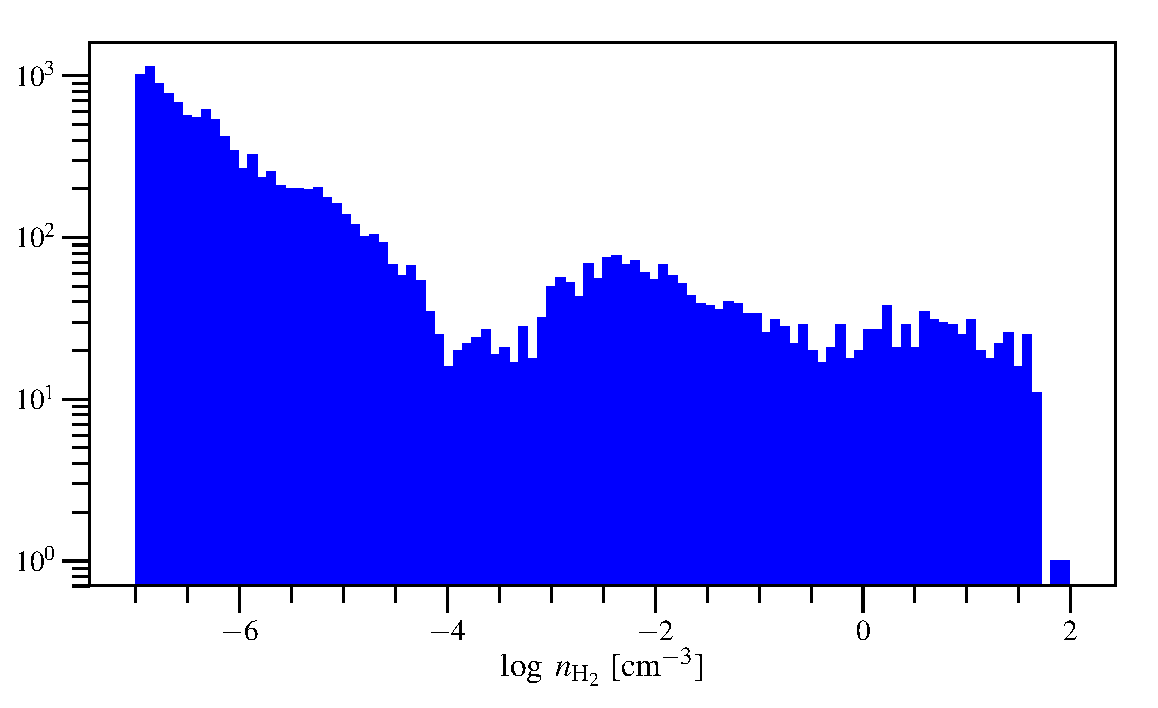
\includegraphics[trim=35 0 10 35, clip, width=0.55\textwidth]{\figpath/hist_test_16.pdf}
\caption{
Volumetric H$_2$ density distribution of \flower taken from a single snapshot, corresponding to the
accretion phase shown in \Fig{SFH}.
\label{fig:h2density}}
\end{figure}


\begin{figure*}[htbp]
 \centering
  \includegraphics[scale=0.6]{\figpath/{dual_16_ncut_0.53}.pdf}
  \\ [-2.9em]
  \includegraphics[scale=0.6]{\figpath/{dual_16_ncut_6.81}.pdf}
  \\ [-2.9em]
  \includegraphics[scale=0.6]{\figpath/{dual_16_ncut_18.96}.pdf}
\caption{
Examples showing the MCs identified in our simulation by applying volumetric H$_2$ density cuts of
$n_{\rm cut}$\eq[0.53, 6.81,19.00]\,cm$^{-3}$, which is only a subset of all the $n_{\rm cut}$ adopted (see text).
    Color shows the H$_2$ surface density, weighted by the column density.
%   \AP{plot a proper label for the colorbar, and remove the trailing right axes labels (that are still there despite our efforts)}\DL{I tried more on Sept 7th, errrr, now all the ticks and labels for both panels disappear... hmm.. Not worth my time to fix this for the report.}
\label{fig:MC}}
% \addtocounter{figure}{-1}
\end{figure*}

In \Fig{h2density}, we show an example of the volumetric H$_2$ density ($n_{\rm H2}$) distribution of \flower
for a given snapshot which includes contributions within $R\sim$\,3.5\,kpc from the galaxy center\footnote{For reference,
the half mass radius of \flower is $\sim$0.5\,kpc and the dark matter virial radius at which the mean enclosed density is 200 times
the critical density of the Universe % presumably defined at the redshift of \flower here?
is $r_{\rm 200}$\ssim15\,kpc.}.
We note that the distribution is almost flat for $n_{\rm H2}\gtrsim1$\,\cc and it samples the range of density
where ``clumps/structures'' are
found based on the Euler characteristic, i.e., the fourth Minkowsky functional (see \citealt{Pallottini17b}).
We identify MCs by applying 10 equally-spaced volumetric H$_2$ density cuts of
$\log{(n_{\rm cut}/{\rm cm^{-3})}}\in[-0.5, 1.5]$\eq[0.32, 0.53, 0.88, 1.45, 2.45, 4.08, 6.81, 11.36, 19.00, 31.62]\footnote{We also vary the range of
$n_{\rm cut}$ adopted and find no qualitative differences
affecting the results and conclusions of this work except in the slope of the CMF (see \Sec{ncut}).}
to the same snapshot
used to plot \Fig{h2density}.

For visualization, we overplot the molecular structures identified using
a subset of the $n_{\rm cut}$ (0.53, 6.81, and 19.00\,\cc) on the H$_2$ density maps
in \Fig{MC} as an example.
The plots shown in \Fig{MC} are weighted by the column density of the total gas content.
% equation below for bookkeeping:
% ${\rm pixel_i}$\eq$\frac{\sum_i~\rho_{\rm H2, i}~w_i~\Delta z_i}{\sum_i~w_i~\Delta z_i}$,
% where $\rho_{\rm H2, i}$ is the H$_2$ density of pixel $i$, $w_i$ is the weighted quantity in pixel $i$ which we adopt
% to be the total gas density, and $\Delta z_i$ is the path length of pixel $i$ along the line-of-sight over which the quantities are integrated along.

Since the molecular structures identified could
easily appear as overlapping structures depending on the viewing angle, we
also plot them in different three-dimensional projections (right panels of \Fig{MC}) --- so that one can more
easily see that they are collections of disjoint structures.
We repeat this identification process for 14 snapshots between
redshift \z$\in$[6.0, 7.2], spaced by $\Delta t$\eq50\,Myr.


Limited by the spatial resolution of our simulation ($l_{\rm cell}\simeq$\,30\,pc), we impose an addition constraint such that an identified structure only survives if it spans at least 10 cells in PPP space. We caution that one caveats of such constraint is that we can only examine the parameter space of ``cloud'' scaling relations at ``cloud'' size $R\gtrsim100$\,pc.



\section{Basic Physics} \label{sec:eqn}
\subsection{Virial Equilibrium and Larson's Relations}  \label{sec:PVE}
% \AP{I fear that putting this subsection here breaks a bit the flow of the analysis of the results. Maybe we can put it as an appendix and keep only eq. 10 in the main text (a put it at when analysing the relevant plot)? }

% Relating Larson's law to stability and pressure (perhaps move this to other section?).
A spherically symmetric cloud of mass $M$ and radius $R$ embedded within
a medium of pressure $P$ is described using the virial theorem:
\begin{equation}
\frac{1}{2}\ddot I = 2(T - T_s) + W + B,
\end{equation}
where $\ddot I$ is the second time derivative of the Lagrangian moment of inertia,
$T$ is the volume term of the total kinetic energy (including thermal and
bulk motions), $T_s$ is the surface term due to external pressure,
$W$ is the gravity term, and $B$ is the magnetic term.
In the case where magnetic field is excluded (i.e., $B$\eq0), we can express this in terms of:
\begin{equation}
\frac{1}{2}\ddot I = 3 M \sigma^2 - \frac{\Gamma GM^2}{R} - 4\pi P_{\rm ext} R,
\label{eqn:virial}
\end{equation}
where the first term on the right hand side (RHS) is the pressure term from velocity dispersion, the second
term is the gravity term, and the third term is the external pressure term.
For the case of simple virial equilibrium (SVE; i.e., equilibrium state without external pressure),
the LHS and the last term on the RHS vanish. The equation becomes:
\begin{equation}
\alpha_{\rm vir} = \frac{3\sigma^2}{\Gamma GM/R} = \frac{5\sigma^2R}{GM},
\label{eqn:alpha}
\end{equation}
where $\Gamma$ is set to 3/5 for a uniform sphere.
We can define
\begin{equation}
V_0^2\equiv\frac{\sigma^2}{R},
\end{equation}
which is related to one of the Larson's relations (linewidth-size relation),
which can be recast into the form of:
\begin{equation}
\sigma^2/R = \pi G \Sigma/5.
\end{equation}
For pressure-bounded virial equilibrium (PVE; i.e. equilibrium state with pressure), % external pressure
Equation~\ref{eqn:virial} becomes:
\begin{equation}
P_{\rm ext} = \frac{3\sigma^2M}{4\pi R^3} - \frac{\Gamma G M^2}{4\pi R^4},
\label{eqn:pext}
\end{equation}
which describes the external pressure needed to confine the gas inside a volume $V$.
Rearranging the equation and substituting $\Sigma$\eq$M/\pi R^2$, we can express
this equation using the following:
\begin{equation}
\frac{\sigma^2}{R} = \frac{1}{3}\left(\frac{4P_{\rm ext}}{\Sigma} + \Gamma G \Sigma \pi \right).
\label{eqn:v0}
\end{equation}
Therefore, for a virialized cloud, one expects a one-to-one mapping between $V_0^2$ and $\Sigma$ since
$\sigma^2/R\propto\Sigma$, whereas
Equation~\ref{eqn:v0} represents the loci along which external pressures $P_{\rm ext}$ are
needed in order for MCs to have linewidths $\sigma$ for a given set of surface densities. % (see\Fig{alpha27}).
In other words, a cloud with $\sigma$ and $\Sigma$ offset from $\sigma^2/R\mapsto\Sigma$
is in equilibrium with the external pressure $P_{\rm ext}$ (and therefore $V_0^2$ is not constant with $\Sigma$ but
varies depending on $P_{\rm ext}$; cf. expectation for SVE, where
$\sigma\propto R^{0.5}$; see e.g., \citealt{Heyer09a, Hughes10a, Hughes13b, Meidt13a}).

We use the virial parameter, which is defined by \Eq{alpha} and describes
the balance between kinetic and gravitational potential energies,
to quantify how stable an MC is.
An $\alpha_{\rm vir}\approx$\,2 corresponds to approximately equipartition between the two energy terms
and is often used to assess the boundedness of a given structure \citep[see e.g., ][]{Kauffmann17b}\footnote{Note, however, that
the true virial state/boundedness of a given structure also depends on the surface terms and the magnetic field (see \Eq{virial}).}.

\subsection{Gravitational Instabilities}   \label{sec:Q}
The onset of gravitational instability is considered to be tightly connected to \SF \citep[e.g.,][]{Kennicutt89a, Wang94a, Li05b, Li06a}.
From virial theorem, Jeans 
instability sets the scales at which gravitational potential overcomes kinetic energy. Namely, gravitational instabilities 
dominates at scales $L > L_J$, where $L_J$ is the Jeans length. 
However, centrifugal force resulting from differential rotation in disk galaxies can 
inhibit collapse even on these scales. As a result, a disk is thought to be 
unstable on scales between $L_J < L < L_{\rm rot}$, where $L_{\rm rot}$ is set 
% \propto \Sigma/B^2
by the surface density of the disk and the angular velocity of the rotation. 

In theoretical and observational works, gravitational instability has been widely discussed in the 
context of the Toomre stability criterion \citep{Toomre64a, Goldreich65b}, or the Toomre $Q$ parameter 
(or the proxy, circular velocity to dispersion ratio; $v_{\rm circ}/\sigma$; e.g., \citealt{GarciaBurillo03a, Genzel11a, Kassin12a, Leung19a}).
% https://ned.ipac.caltech.edu/level5/March15/Glazebrook/Glazebrook5.html
%
% from linear analysis
For {\it axisymmetric} mode ($m$\eq0), the dispersion relation for the growth of density perturbation in a rotating turbulent disk
of finite thickness $h$ 
is described by:
\begin{equation}
\omega^2 = \kappa^2 - \frac{2\pi G \Sigma |k|}{1 + |k| h} + \sigma^2 k^2,
\label{eqn:3Ddisp}
\end{equation}
where $k$ is the wavenumber and $\kappa$ is the epicyclic frequency, defined as:
\begin{equation}
\kappa^2\equiv\frac{2\Omega}{R}\frac{d}{dR}\left(R^2\Omega\right).
\label{eqn:kappa}
\end{equation}
% \kappa\propto\Omega
The first term on the RHS of Equation~\ref{eqn:3Ddisp} describes rotation support, whereas the second term describes self-gravity, and
the third term describes pressure support.
One can then define the so-called Toomre-Q parameter as:
\begin{equation}
Q\equiv\frac{\sigma\kappa}{\pi G \Sigma}.
\label{eqn:Q}
\end{equation}
For $kh\ll1$, Equation~\ref{eqn:3Ddisp} reduces to the thin disk approximation, which 
becomes unstable % perturbation grows exponentially in time
for some $k$ when $\omega^2 < 0$ (or equivalently, $Q < 1$; \citealt{Toomre64a}).
Under this condition (i.e., when local gravitational instability 
overcomes support from pressure and rotation), fragmentation {\it can} happen. 
% but further evolution depends on their EOS.
%(e.g., instability impose by angular momentum from gas accretion from the cosmic web and
%satellite galaxies and stellar feedback).
% Note that fragmentation is expected to happen at critical scale length 
% $\lambda_{\rm crit} < 2 \pi^2 G \Sigma / \kappa^2$, which is greater than the typical size of 
% GMCs. It should be clear that the instability sets the scales for fragmentation, but 
% star-forming GMCs are the collapsing, denser, and cooler molecular structures on even smaller scales.
% The fragmented structures thus correspond to regions where $Q\lesssim1.
Similarly, for a collisionless fluid, the Toomre $Q$ parameter is defined by:
\begin{equation}
Q\equiv\frac{\sigma\kappa}{3.36 G \Sigma}
\end{equation}
\citep{Toomre64a}.

To account for stabilizing effect of both gas and stars and the non-negligible disk thickness, 
% since thickness of a disk weakens the gravitational forces within the disk plane and lower the values for $Q$
% Romeo:  The effect of thickness is to increase the stability parameter of each 
% component by a factor T, which depends on the ratio of vertical to radial velocity dispersion, following eqn 8 of their paper.
we consider the approximation for the effective two-component $Q_{\rm eff}$ parameter following \citet{Romeo11a} and
\citet{Inoue16a} which is expressed as follows:
\begin{equation}
Q^{-1}_{\rm eff} = \[ \left\{
				\begin{array}{lccr}
					     {\displaystyle\frac{w}{T_{\rm star} Q_{\rm star}} + \frac{1}{T_{\rm gas} Q_{\rm gas}}}      & & & \mbox{if\ }T_{\rm star} Q_{\rm star} \geq T_{\rm gas} Q_{\rm gas} \\ [0.75em]
                                               {\displaystyle\frac{1}{T_{\rm star} Q_{\rm star}} + \frac{w}{T_{\rm gas} Q_{\rm gas}}}      & & & \mbox{if\ }T_{\rm star} Q_{\rm star} \leq T_{\rm gas} Q_{\rm gas} \\				
				\end{array} 
			    \right,
			    \]
\end{equation}
where $w$ is defined as:
\begin{equation}
w\equiv\frac{2 \sigma_{\rm star} \sigma_{\rm gas}}{\sigma_{\rm star}^2 + \sigma_{\rm gas}^2},
\end{equation}
and $T$ is approximated as:
\begin{equation}
T = \[ \left\{
		\begin{array}{lccr}
			{\displaystyle 0.8 + 0.7\left(\frac{\sigma_{z}}{\sigma_{r}}\right)}      && & \mbox{if\ } \sigma_z \lesssim 0.5 \times \sigma_r \\ [1.25em]
			{\displaystyle 1 + 0.6\left(\frac{\sigma_{z}}{\sigma_{r}}\right)}        & & & \mbox{if\ } \sigma_z \gtrsim 0.5 \times \sigma_r 
\\
		\end{array}
	\right \rlap{.}
	\]
\end{equation}

For the purpose of this work, we present Toomre $Q$ map in \Sec{results} and discuss the 
importance of support from galactic rotation and shear against axisymmetric perturbations in \Sec{origin}.




\subsection{Key Properties of Clouds}  

% Molecular clouds are the natal place for \SF, their structure and dynamics hold important clues to understanding
% the mechanisms and physics of formation and evolution of molecular structures and \SF.
In next section, we examine and compare properties of the MCs with
observations in the context of the Larson's relations \citep{Larson81a}. 
Namely, the linewidth-size, density-size, and mass-size relations.
Larson's relations are adopted for the discussion in this work as they 
describe the interactions between gravity and turbulence, and is the first set of
relations used for studying star-forming molecular structure formation based on observables
which has been routinely used for comparing properties of molecular structures in different galactic environments.
% Inner MW: R=2-8.5 kpc, most of the mass in the molecular ISM is in the form of GMCs with sizes $gtrsim$20\,pc and masses greater than 10$^5$\,\Msun \citep{Sanders85a}.

Upon identifying the molecular structures, we extract properties such as
mass ($M_{\rm cl}$),
size ($R$),
Mach number ($\mathcal{M}$), velocity dispersion ($\sigma$), and
gas surface density ($\Sigma_{\rm gas}$)
to examine their dynamics.

The mass of an MC is calculated from the uniformly-gridded 3D density field,
integrating over all zones of the MC, multiplied by its volume.
The size of an MC ($R$) is defined assuming spherical geometry (i.e.,
the size is parameterized via the radius of a sphere, which has a volume corresponding to that of the identified MC).
% {\AP The size is an effective radius, calculated from the total volume of the MC assuming spherical symmetry.}
Since in \obs, dense gas contributes more to the observed linewidths than the more diffuse gas. We therefore calculate
the non-thermal component of the velocity dispersion ($\sigma_{\rm NT}$) of each MC as a density-weighted quantity:
\begin{equation}
\sigma_{\rm NT}^2 = \frac{1}{{3}}\frac{\sum_{i} \rho_i \left|\mathbf{v}_i - \mathbf{\bar v}\right|^2}{\sum_i \rho_i}\,,
\end{equation}
which is summed over the cells composing each MC.
The total velocity dispersion includes contributions from the thermal sound speed ($c_s$):
\begin{equation}
\sigma^2 = \sigma_{\rm NT}^2 + c_s^2.
\end{equation}
The local sound speed of all identified molecular complexes are much smaller compared to the their
turbulent velocities\footnote{We find comparable velocity dispersion between that derived from
taking the root mean square versus that derived from thermal and non-thermal pressure terms, indicating that
rotation velocity is unlikely to be the dominant source of velocity dispersion reported here.
% We further quantify the contributions arising from galactic rotation and shear to the extracted velocity dispersions of the MCs in \Sec{Q}.
In the subsequent sections, we adopt the root mean square of the velocity field
as the velocity dispersion ($\sigma$). \label{ftn:veldisp}}.
On average, the Mach number of the MCs corresponds to about $\mathcal{M}\approx50$.
This is consistent with the global analysis done on \flower by \citet{Vallini18a}.


We show in \Fig{dist} the MC distributions in terms of their
molecular gas masses, radii, and gas mass fractions, which we define as
\begin{equation}
f_{\rm gas} = \frac{M_{\rm H2}} {\left(M_{\rm H2} + M_*\right)},
\end{equation}
where $M_*$ is the stellar mass.
We note that the distributions vary for different snapshots, depending on the evolutionary stage of \flower.
The highest density threshold of $n_{\rm cut}$\eq31.62\,\cc yields a ``minimum'' MC mass of
the order of 10$^{6.5}$\,\Msun for the densest MC.
% {\AP  maybe we can tie it to the mass resolution limitation imposed by our criterion.}
We find $\sim$10$-$13 MCs with masses exceeding 10$^8$\,\Msun across all the
snapshots for each of the given $n_{\rm cut}$ (see \Sec{method}).
The mass of the MCs identified ranges between $M_{\rm cl}\approx$10$^{6.5-9}$\,\Msun, 
consistent with those observed in \z$\sim$2 galaxies in
rest-frame {\it UV and optical light} \citep{Elmegreen07a, Elmegreen09a}.

\begin{figure*}[htbp]
\centering
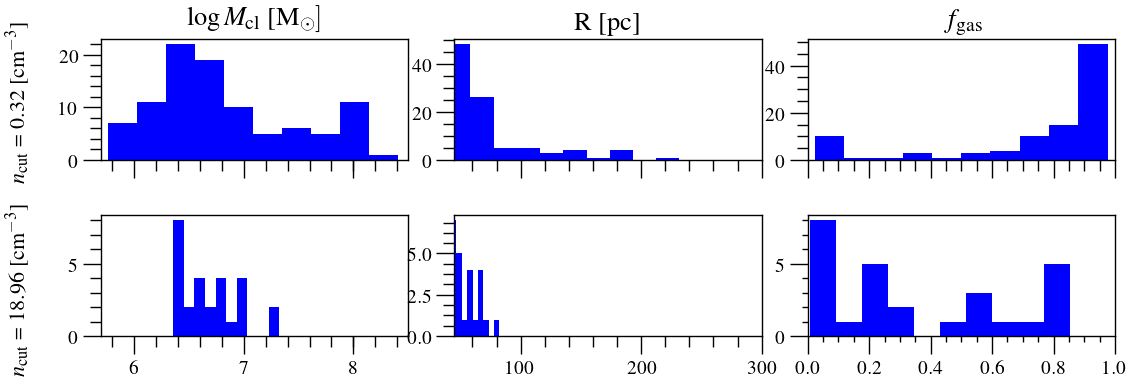
\includegraphics[trim=0 0 0 0, clip, width=0.85\textwidth]{\figpath/minmaxNcut_basicDistributions.png}
\caption{
Distributions of mass, size, and gas mass fraction of MCs identified using
the lowest $n_{\rm cut}$ (left panels) and $n_{\rm ncut}$\eq18.96\,\cc (right panels).
Note that the scale shown on the y-axes are different between the left and right panels, as less MCs are identified
at higher $n_{\rm cut}$.
\label{fig:dist}}
\end{figure*}



\section{Results: MC Properties and Cloud Scaling Relations}    \label{sec:results}
\subsection{Single Snapshots}  \label{sec:singless}

For each of the two most extreme evolutionary stages of \flower\ --- accretion and starburst phase (see \Sec{sfh}),
we identify a set of MCs. 
Scaling relations for the MCs identified in the accretion phase are shown in top panels 
of \Fig{larsons_single}, \Fig{alpha16}, and \Fig{alpha27}, and in the bottom panels for the starburst phase.
Regardless of the H$_2$ density cuts adopted,
the MCs are found to have consistently high turbulences and surface densities in both stages.
These correspond to MCs at the center of the main disk of \flower and
occupy the top right corner of the Larson's relation shown in \Fig{larsons_single}.
As we increase the density threshold, some of the MCs within the main disk break
into multiple sub-MCs.
As such, we effectively identify a population of denser molecular structures (see \Fig{MC}).

% PVE
We also compare the MCs identified in our simulations to
those observed in the Milky Way in the context of the $\sigma^2/R - \Sigma$ relation (see \Fig{alpha27}). 
The V-shaped dashed lines in the figure show the loci along which the given external pressures are needed for
MCs to have linewidth for a given set of surface densities (see \Sec{PVE}).
% (Rice+16) find variation in $V_0^2$, where they find larger linewidths for GMCs in inner galactic disk, but they find that the clouds in the Galactic disk are still consistent with SVE (see also Solomon87a ; cf. Heyer+09).
The MCs in the satellite galaxies are found to follow the locus of $\log{(P/\textrm{K cm}^{-3})}$\eq6 (see \Fig{alpha27}).


\begin{figure*}[htbp]
\centering
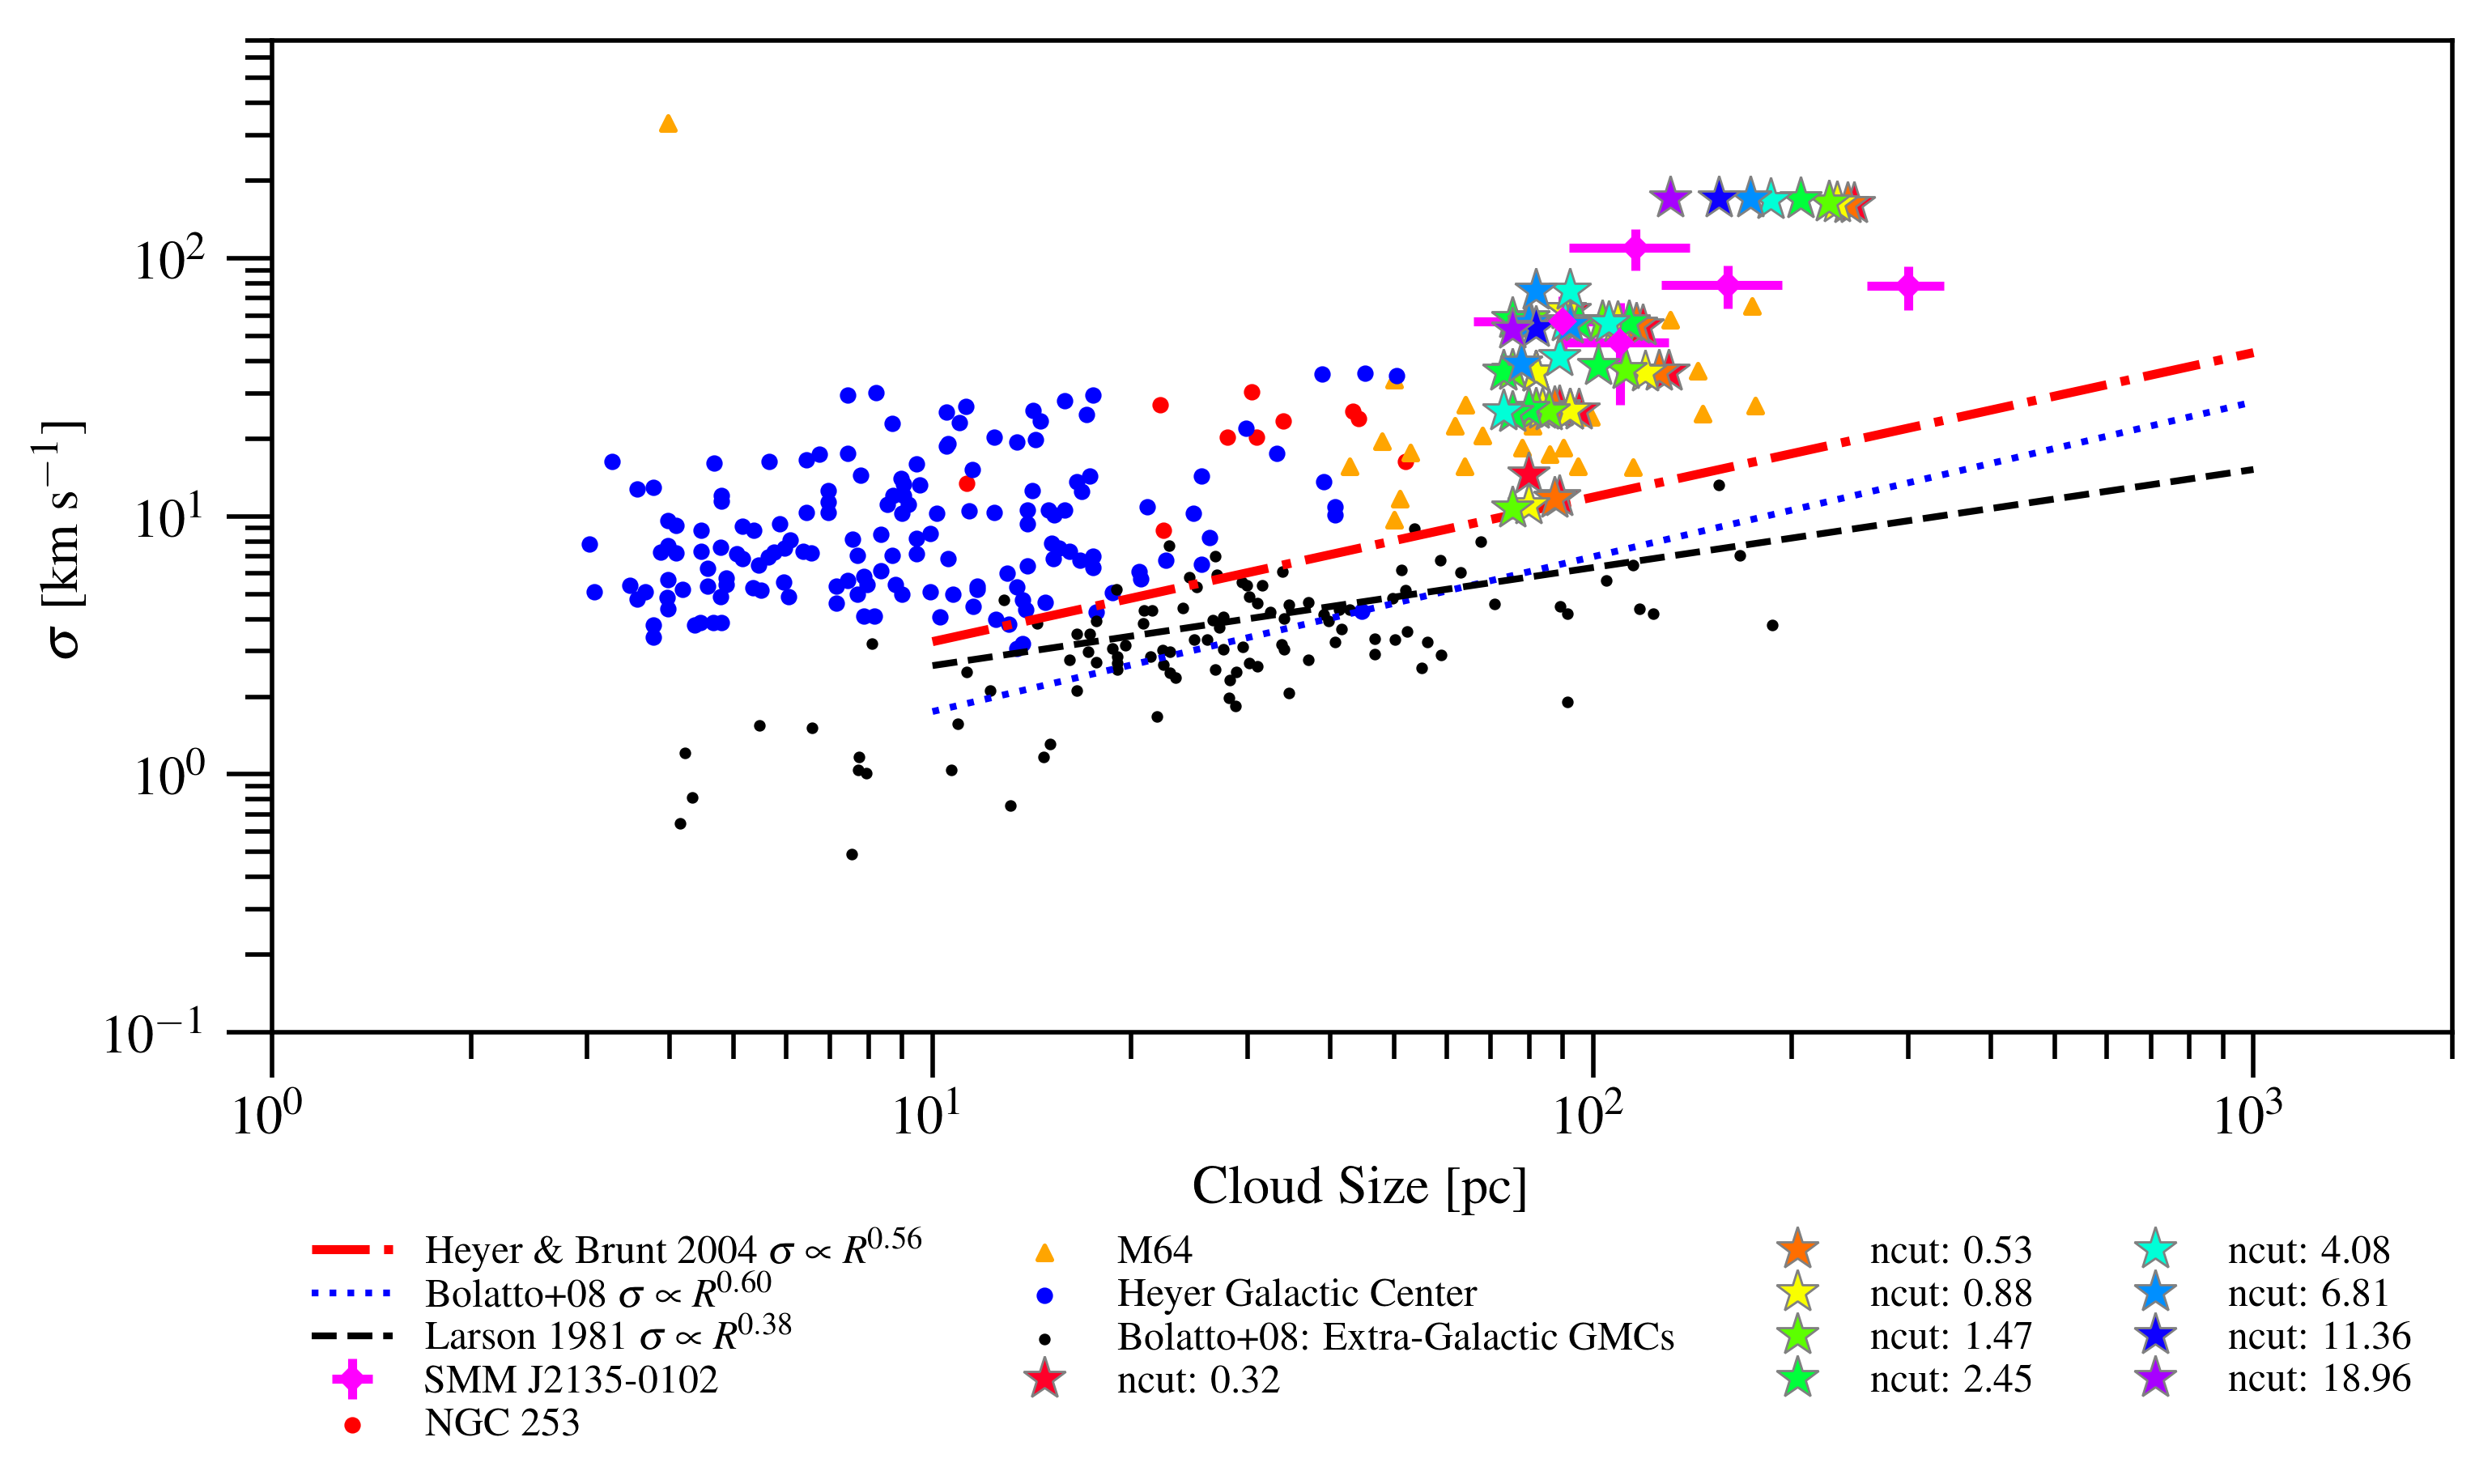
\includegraphics[trim=0 0 0 0, clip, width=0.85\textwidth]{\figpath/ss16_larsons.png}
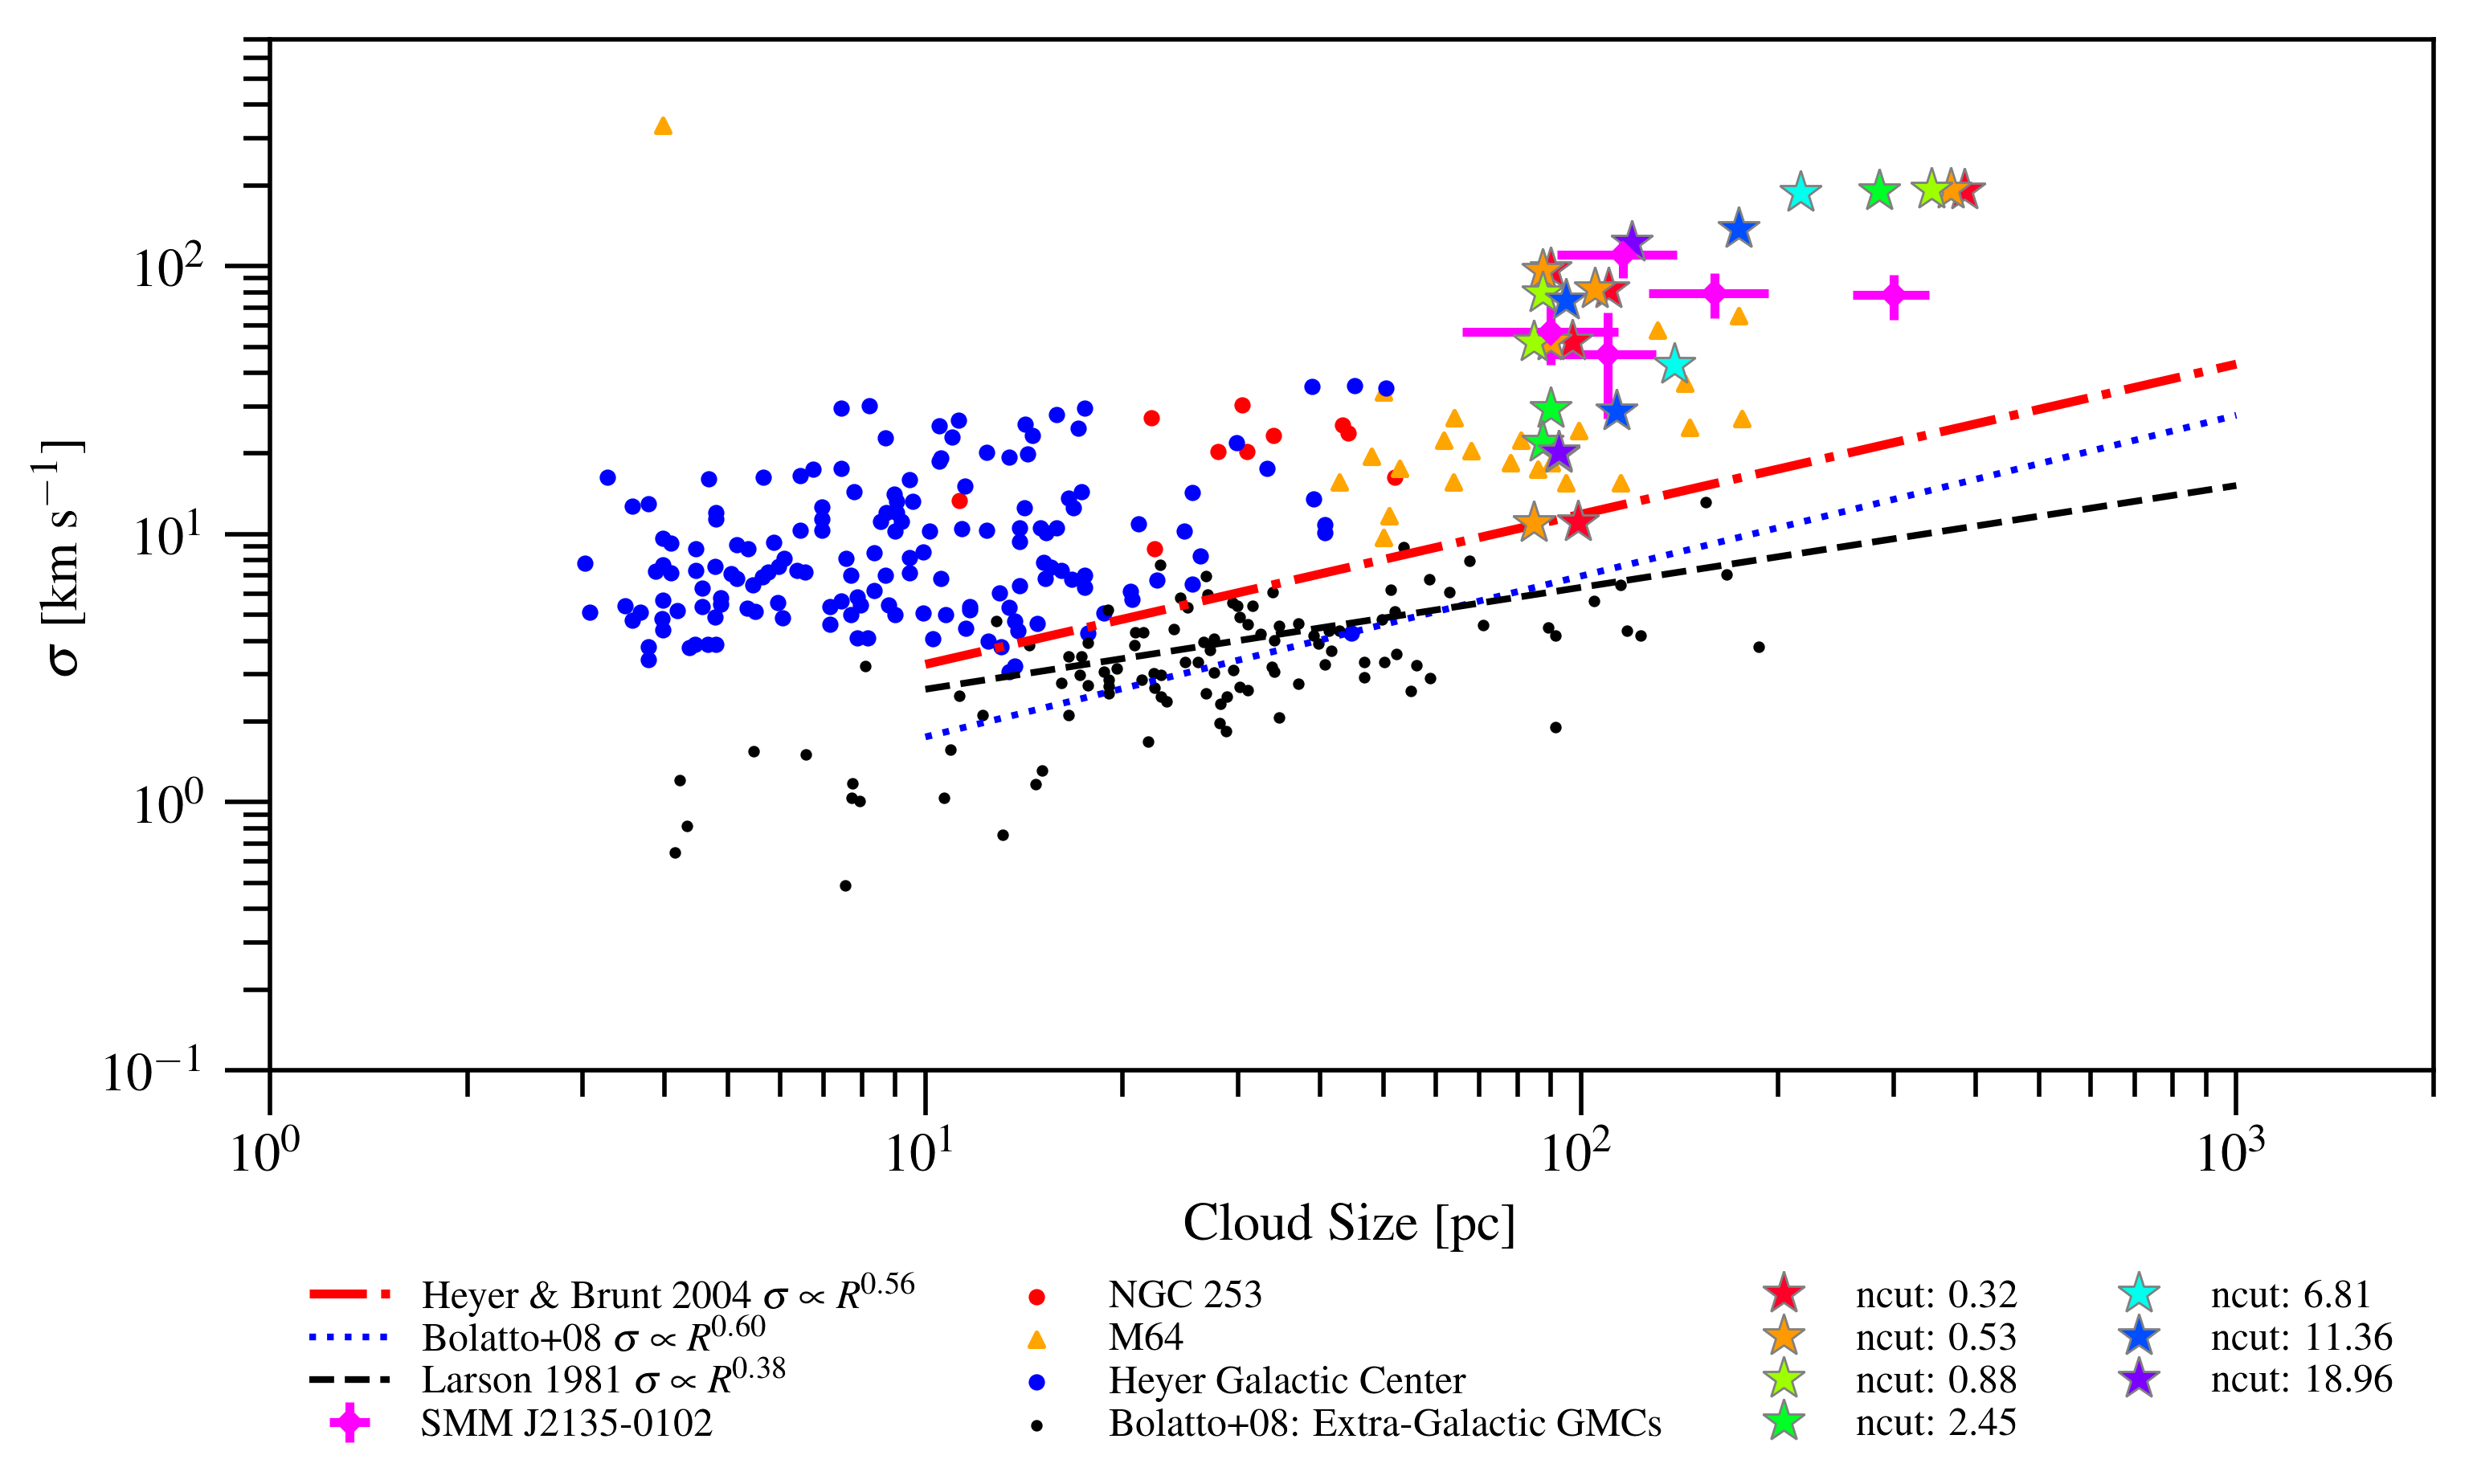
\includegraphics[trim=0 0 0 0, clip, width=0.85\textwidth]{\figpath/ss27_larsons.png}
\caption{
Larson's (linewidth-size) relation of \flower in
accretion phase (top) and
starburst phase (bottom) compared to
those observed in nearby and the \z$\sim$2 star-forming galaxy.
% Red lines show the relation obtained from \citet{}.
Literature data and empirical relations are compiled from \citet{Larson81a, Heyer04a, Rosolowsky05a, Bolatto08a, Swinbank11a, Leroy15a}.
\label{fig:larsons_single}}
\end{figure*}


\begin{figure*}[htbp]
\centering
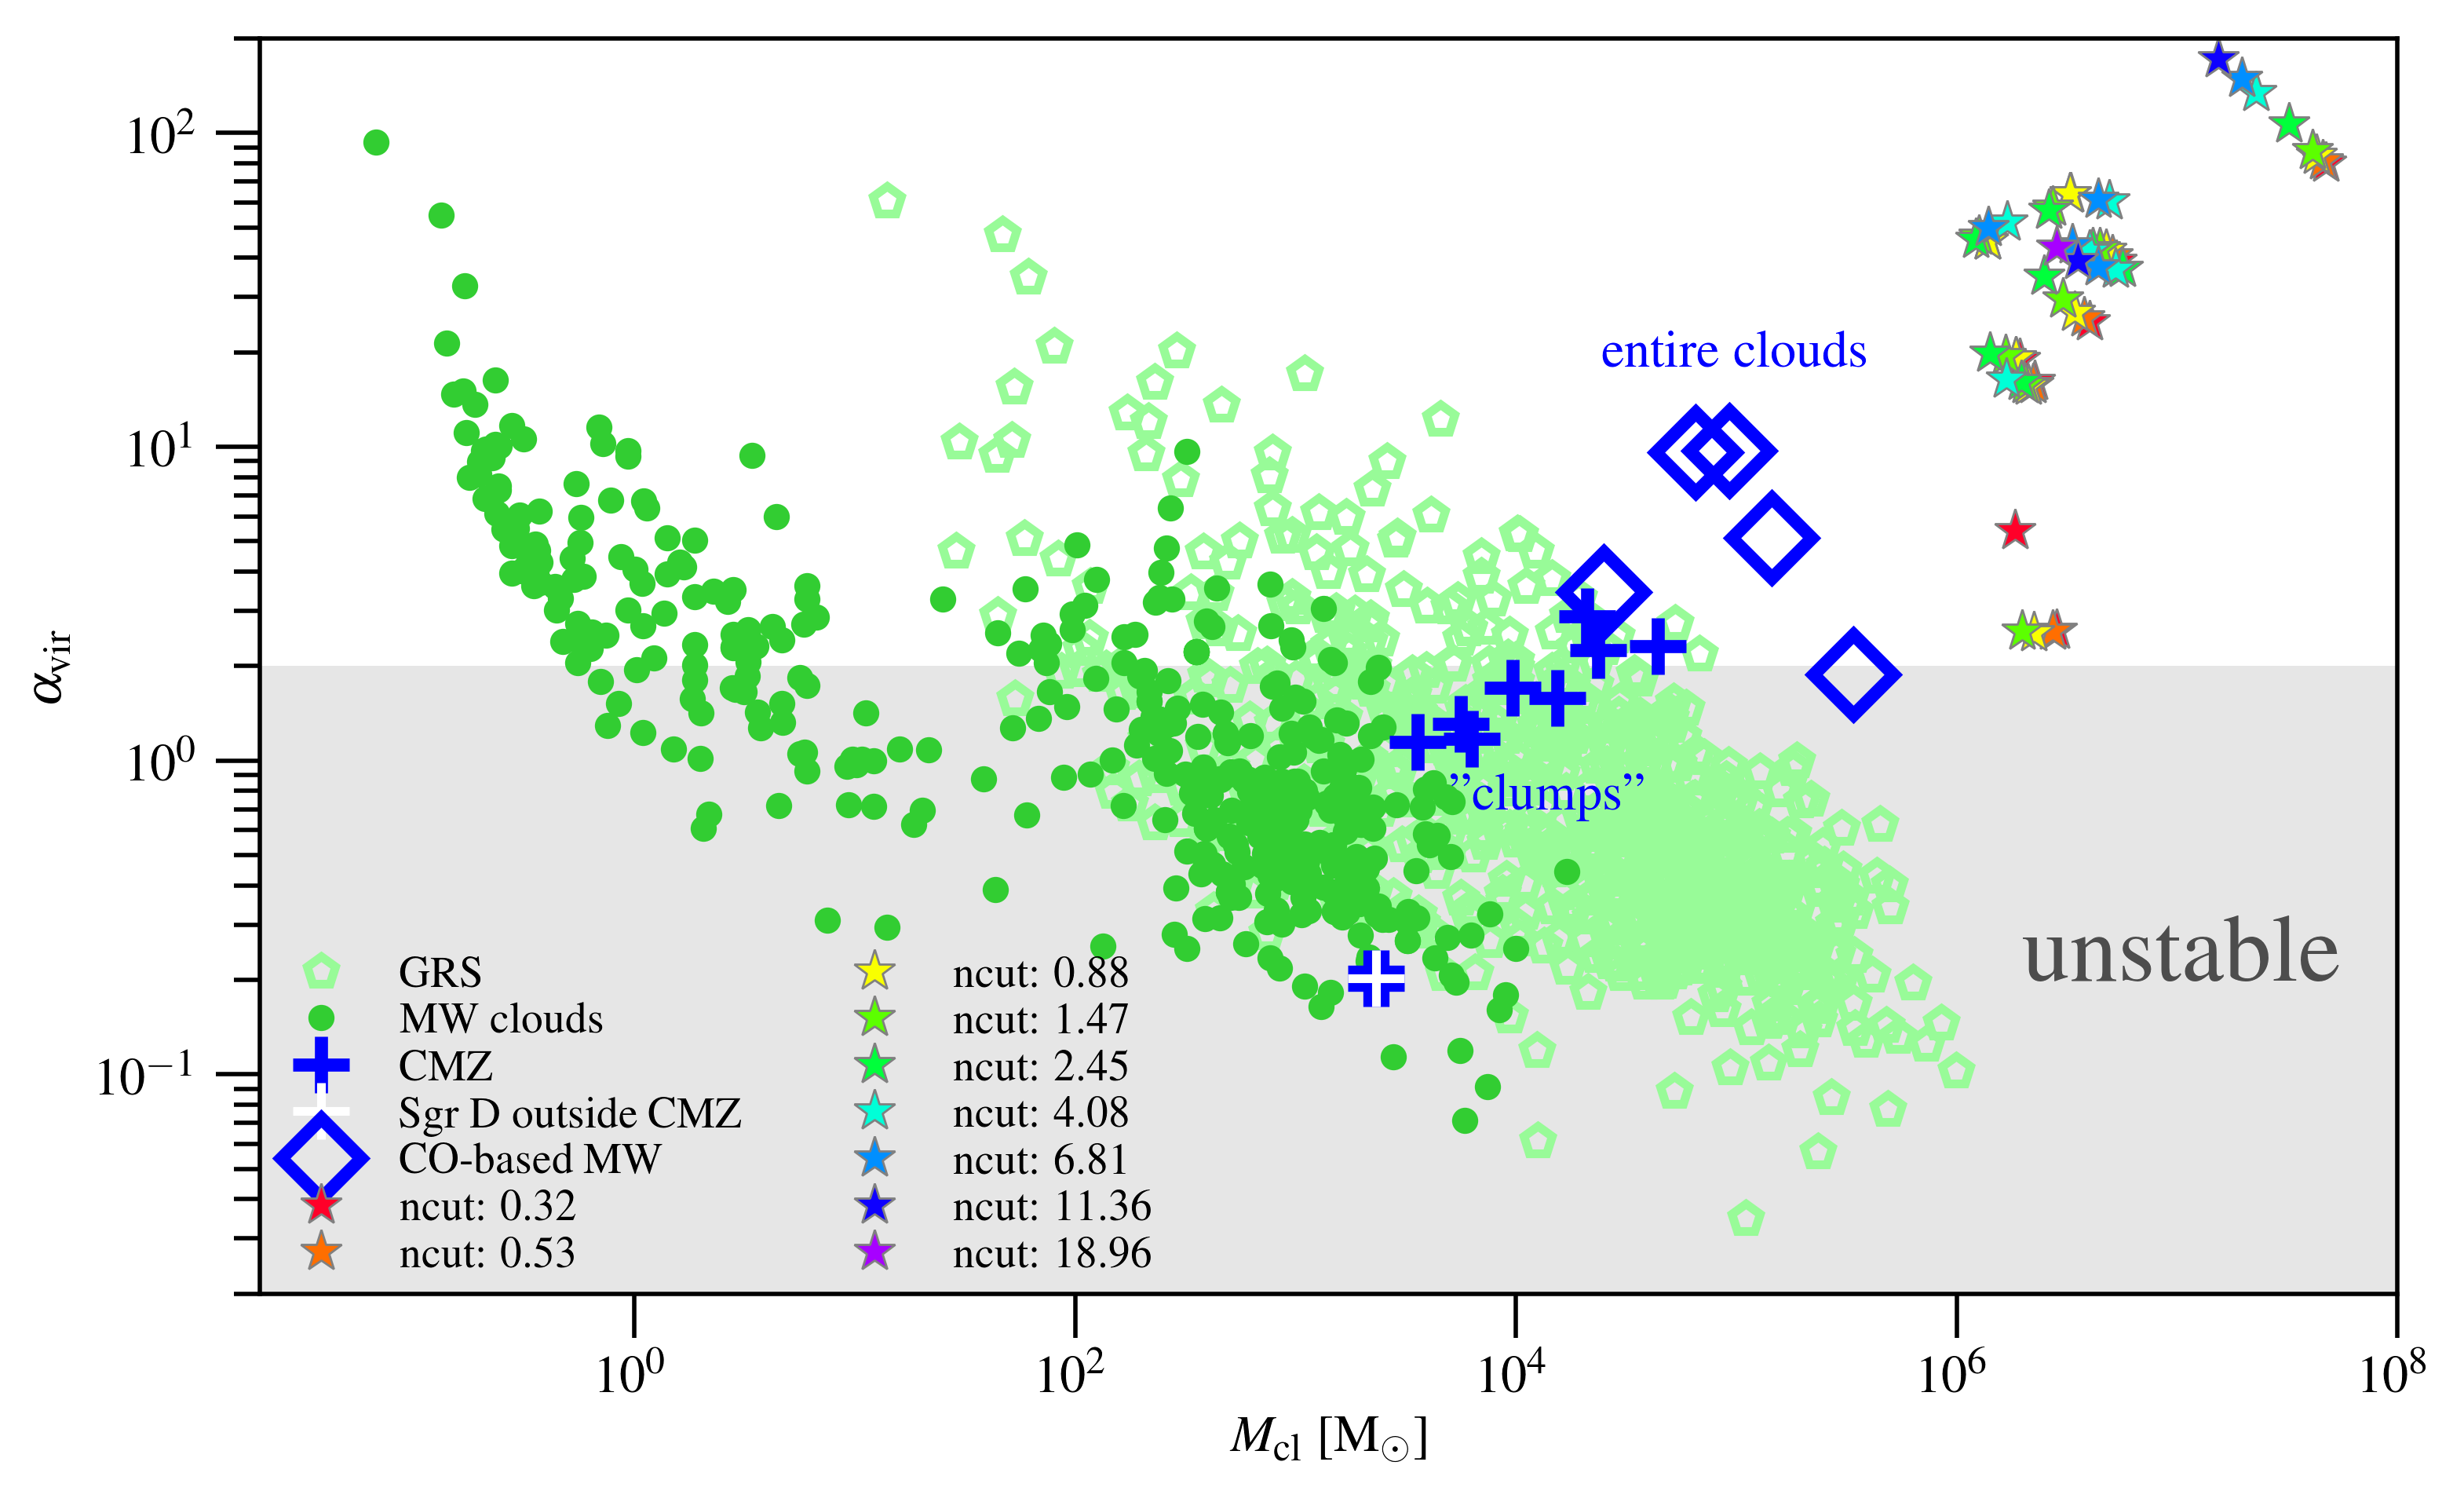
\includegraphics[trim=0 0 0 0, clip, width=0.65\textwidth]{\figpath/ss16_alphavir.png}
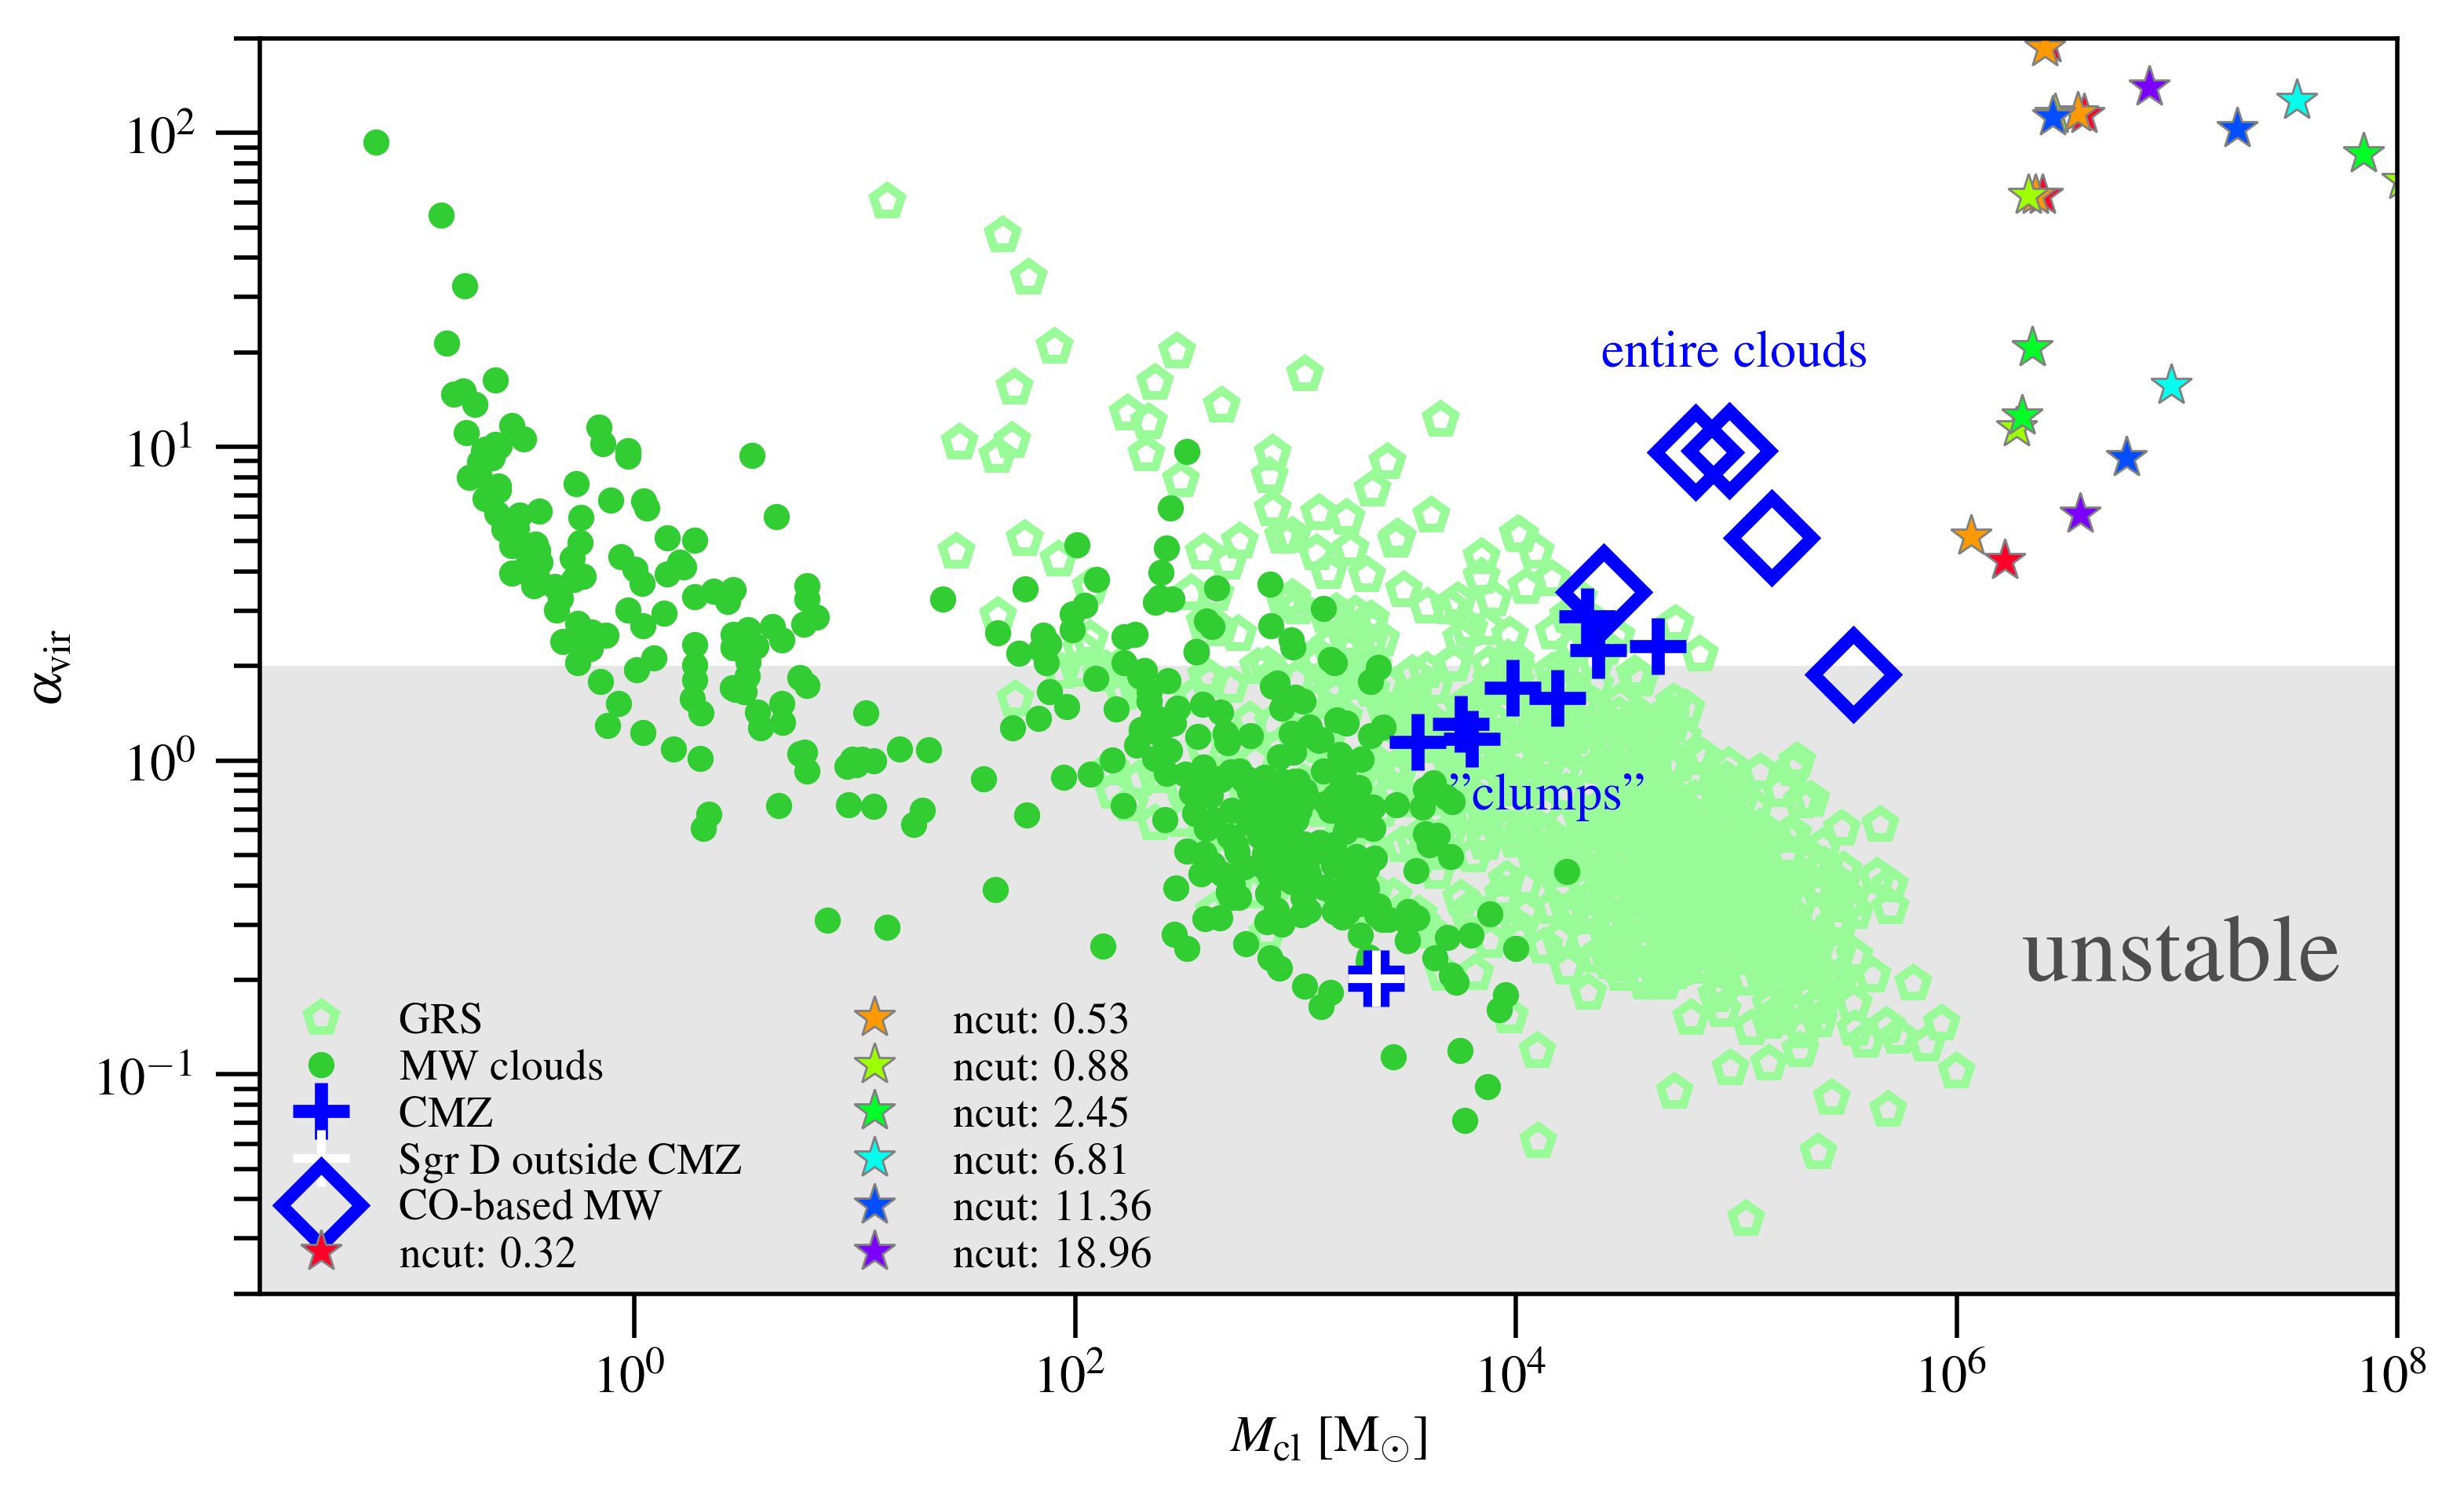
\includegraphics[trim=0 0 0 0, clip, width=0.65\textwidth]{\figpath/ss27_alphavir.png}
\caption{
Virial parameter and cloud mass of \flower (star symbols) in the accretion phase (top panel) 
and the starburst phase (bottom panel) compared to the 
Milky Way (other symbols).
Literature data are compiled from \citealt{Kauffmann17b} and references therein.
Star symbols are color-coded by $n_{\rm cut}$.
Star symbols lying close to $\alpha_{\rm vir}\approx2$ correspond to MCs in the satellite galaxies.
\label{fig:alpha16}}
\end{figure*}


\begin{figure*}[htbp]
\centering
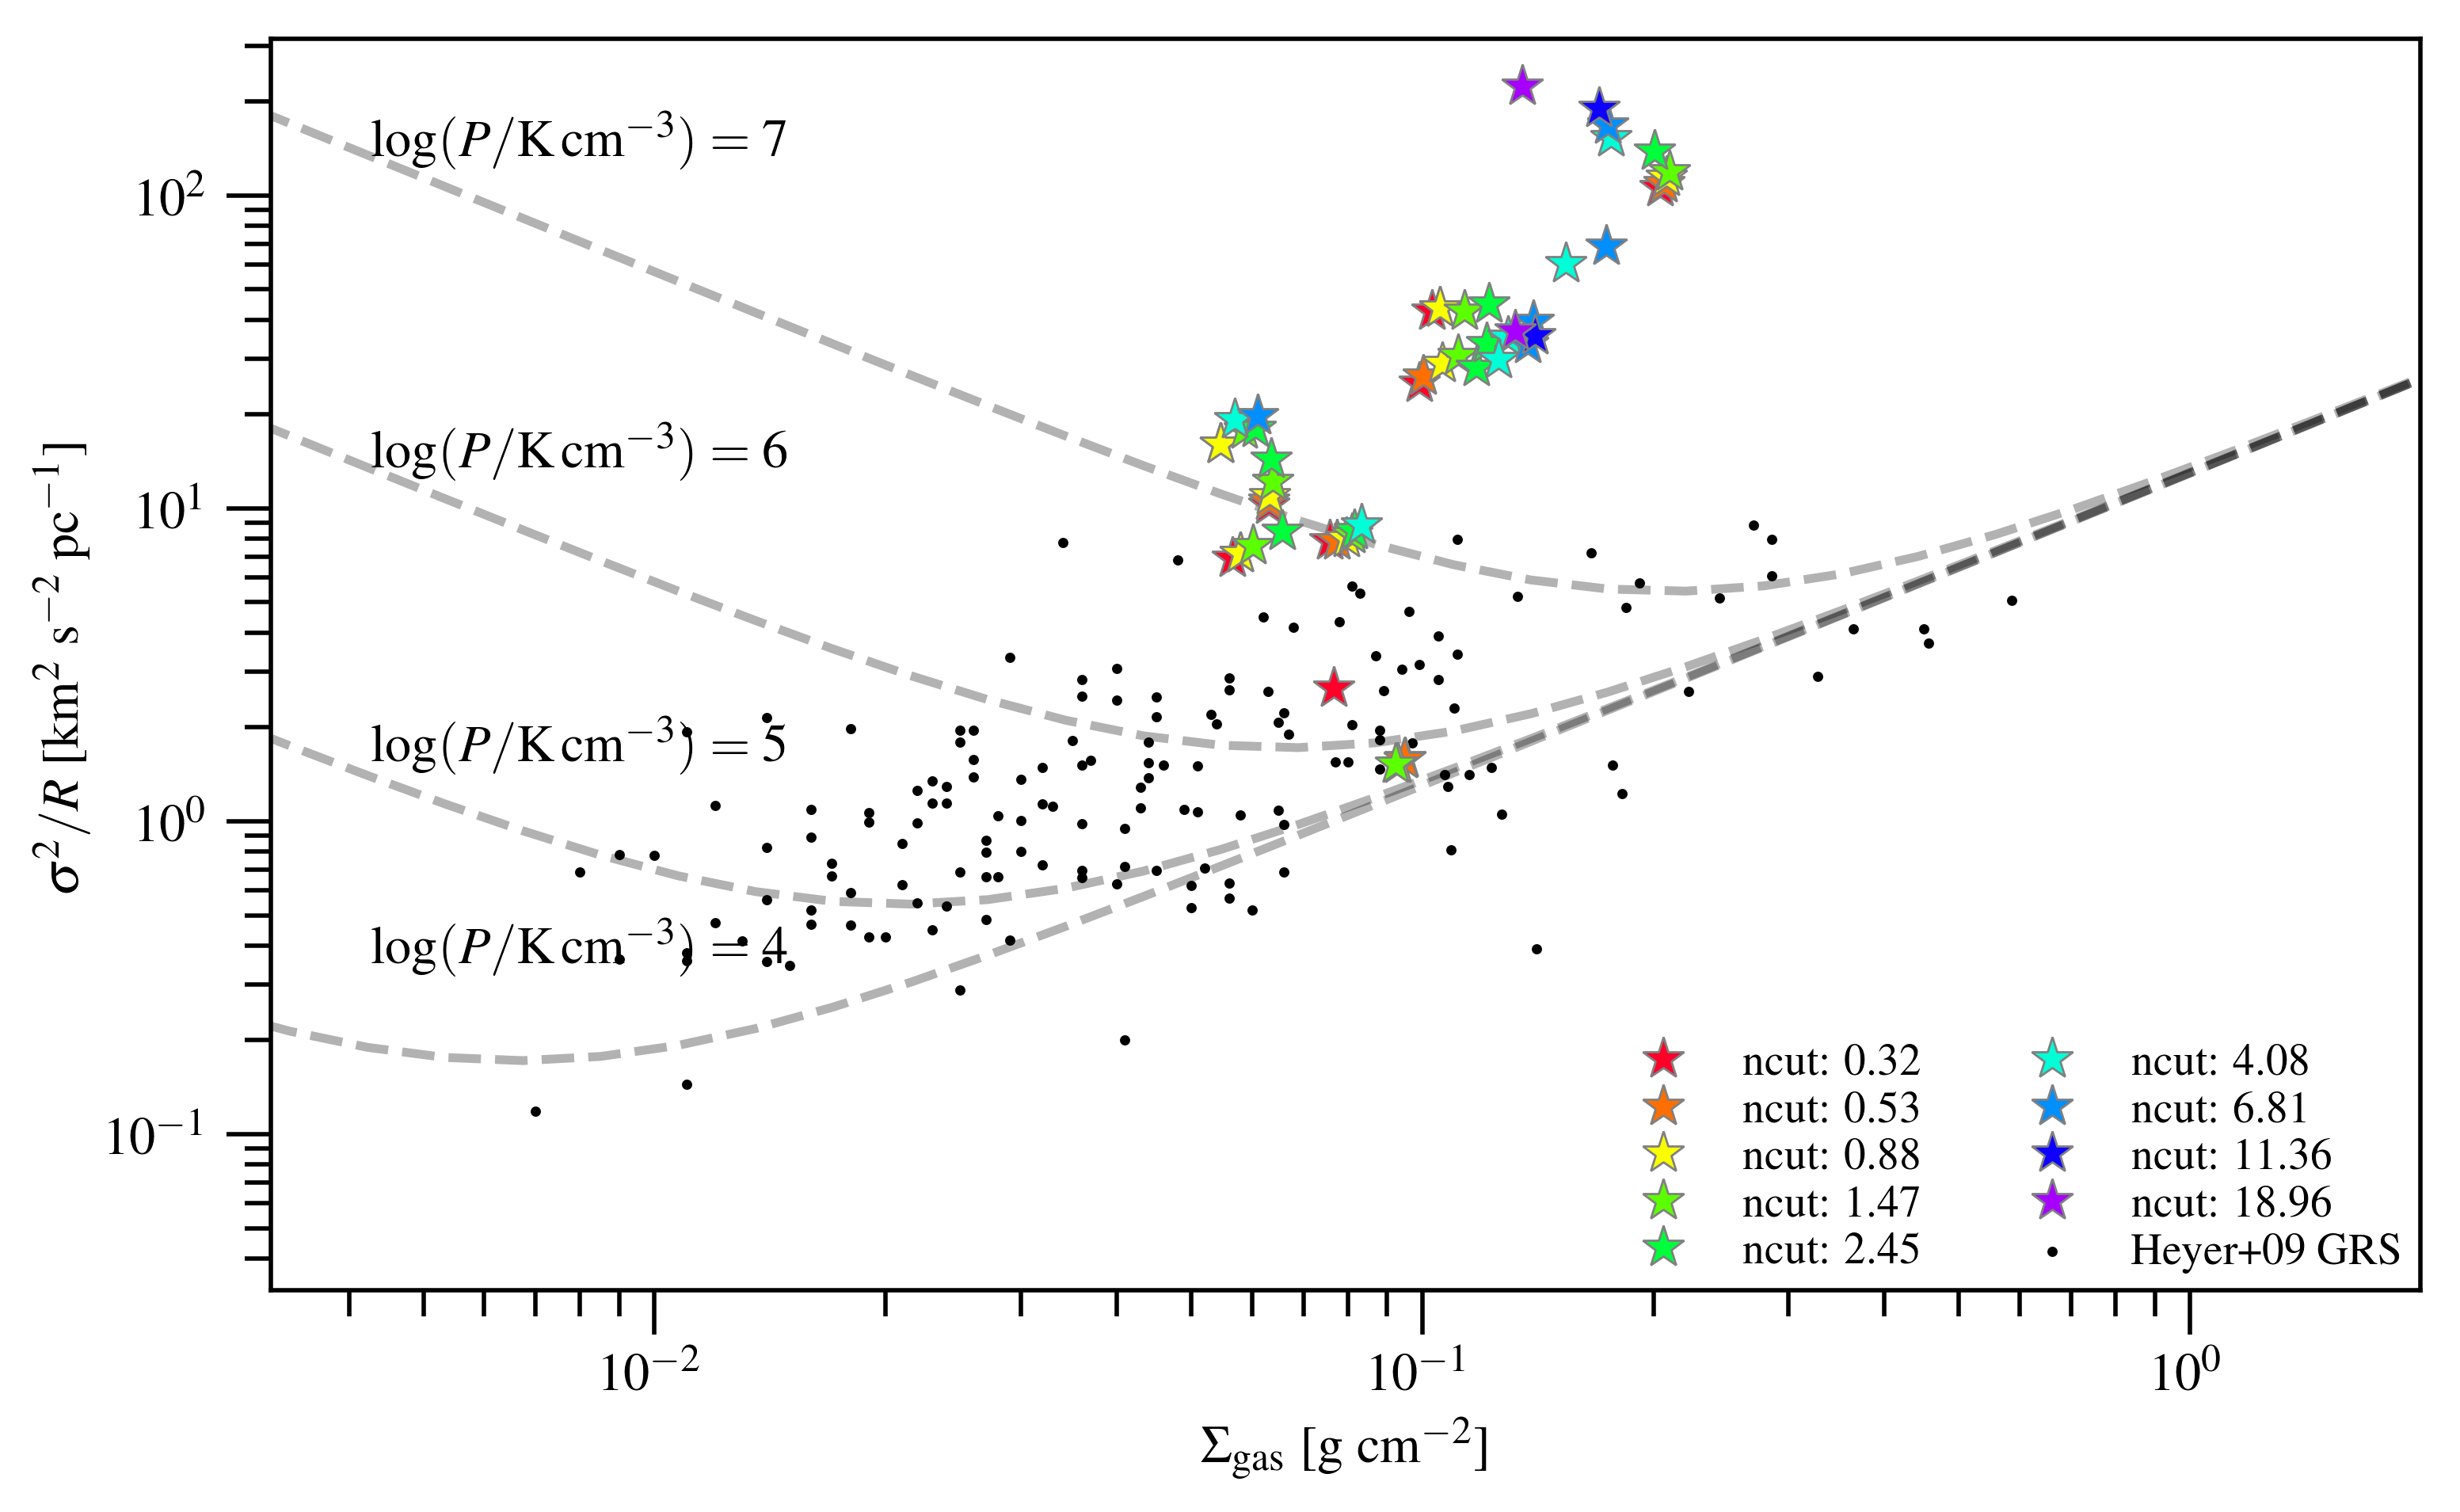
\includegraphics[trim=0 0 0 0, clip, width=0.65\textwidth]{\figpath/ss16_PVE.png}
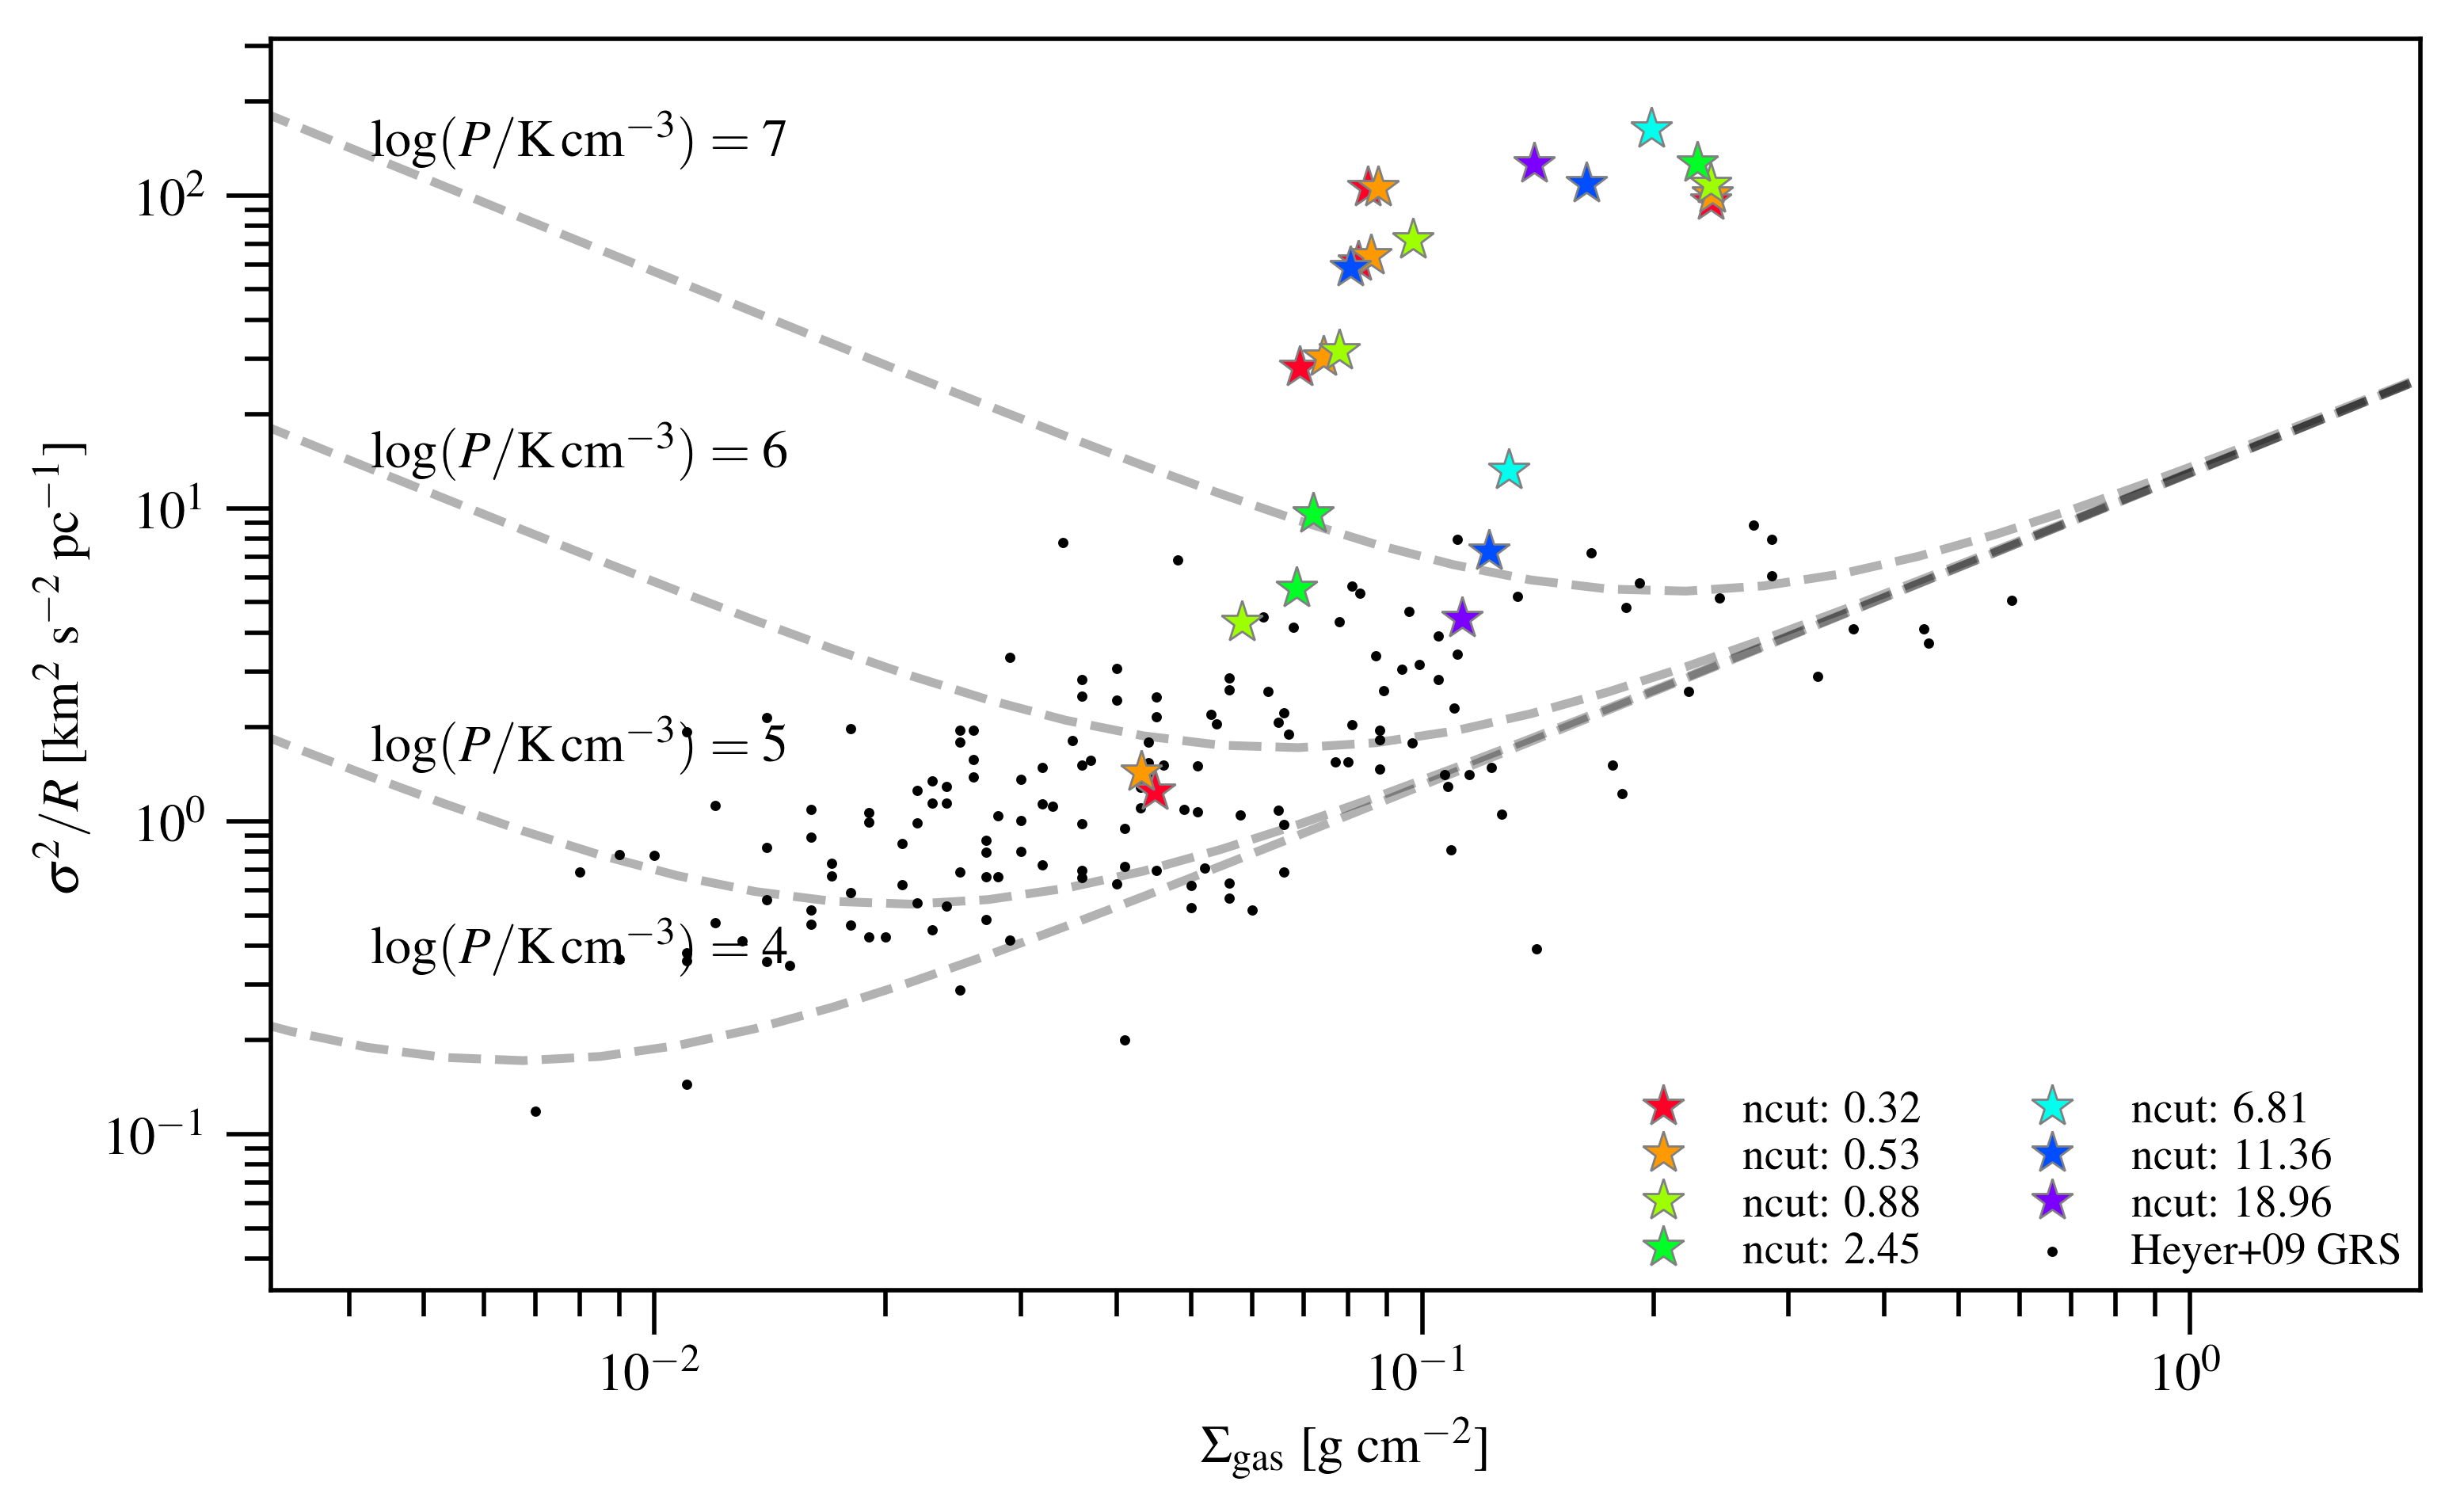
\includegraphics[trim=0 0 0 0, clip, width=0.65\textwidth]{\figpath/ss27_PVE.png}
\caption{
$\sigma^2/R - \Sigma_{\rm gas}$ relation of the MCs identified in our simulation (star symbols)
in the accretion phase (top panel) and the starburst phase (bottom panel)
compared to those observed in the Milky Way (black dot markers; \citealt{Heyer09a}).
The V-shaped dashed lines show the loci along which the given external pressures
are needed for MCs to have linewidth $\sigma$ for a given set of surface densities (see \Sec{PVE}).
Similar to \Fig{alpha16}, star symbols are color-coded by $n_{\rm cut}$.
Star symbols along the locus of $\log{(P/\textrm{K cm}^{-3}) = 6}$
correspond to MCs in the satellite galaxies.
\label{fig:alpha27}}
\end{figure*}





% cloud structures at large and small scale
% Larson's: m = 460 M_sun (r_pc)^1.9 for structure w/in molecular clouds. --> $m \propto r^2$ \citep{McKee07a} (law of constant
% column density) as fundamental properties of molecular cloud structure.
Larson's third relation describes fundamental properties of molecular clouds, relating their structures on small and large scales
via two physical properties: mass and size \citep{Larson81a, McKee07a}. This is also known as the law of constant column density,
since cloud mass in \obs is sometimes derived by integrating
over the mass surface density ($\Sigma$), which is related to the column density ($N_{\rm H2}$) obtainable from extinction maps ($A_V$).
That is, $N_{\rm H2}\propto A_V$, $\Sigma\propto N_{\rm H2}$, and $M$\eq$\int \Sigma~dA$.
Therefore, cloud mass is related to $N_{\rm H2}$ and $A_V$.

We show in \Fig{MR} the size-mass relation of the MCs of \flower % in its accretion phase 
compared to
observational data of molecular clouds in the Milky Way that are found to be associated with massive \SF
\citep{Beuther02a, Mueller02a, Hill05a, Motte07a} and an empirical relation obtained for massive \SF based on
Milky Way clouds ($<$10\,\Msun; \citealt{Kauffmann10b, Kauffmann10c} and references therein): $M \gtrsim 870$\,\Msun$\times\,\left(r/{\rm pc}\right)^{1.33}$.
In the same plot, we also show loci of constant surface densities, which are parameterized through the visual extinction $A_V$.
As shown in \Fig{MR}, the MCs identified 
% in the accretion phase of 
in \flower lie above this relation, along the locus
with a visual extinction of $A_V$\eq4\,mag \citep{Lombardi10a}.
We discuss this result in the following section.

\begin{figure*}[htbp]
\centering
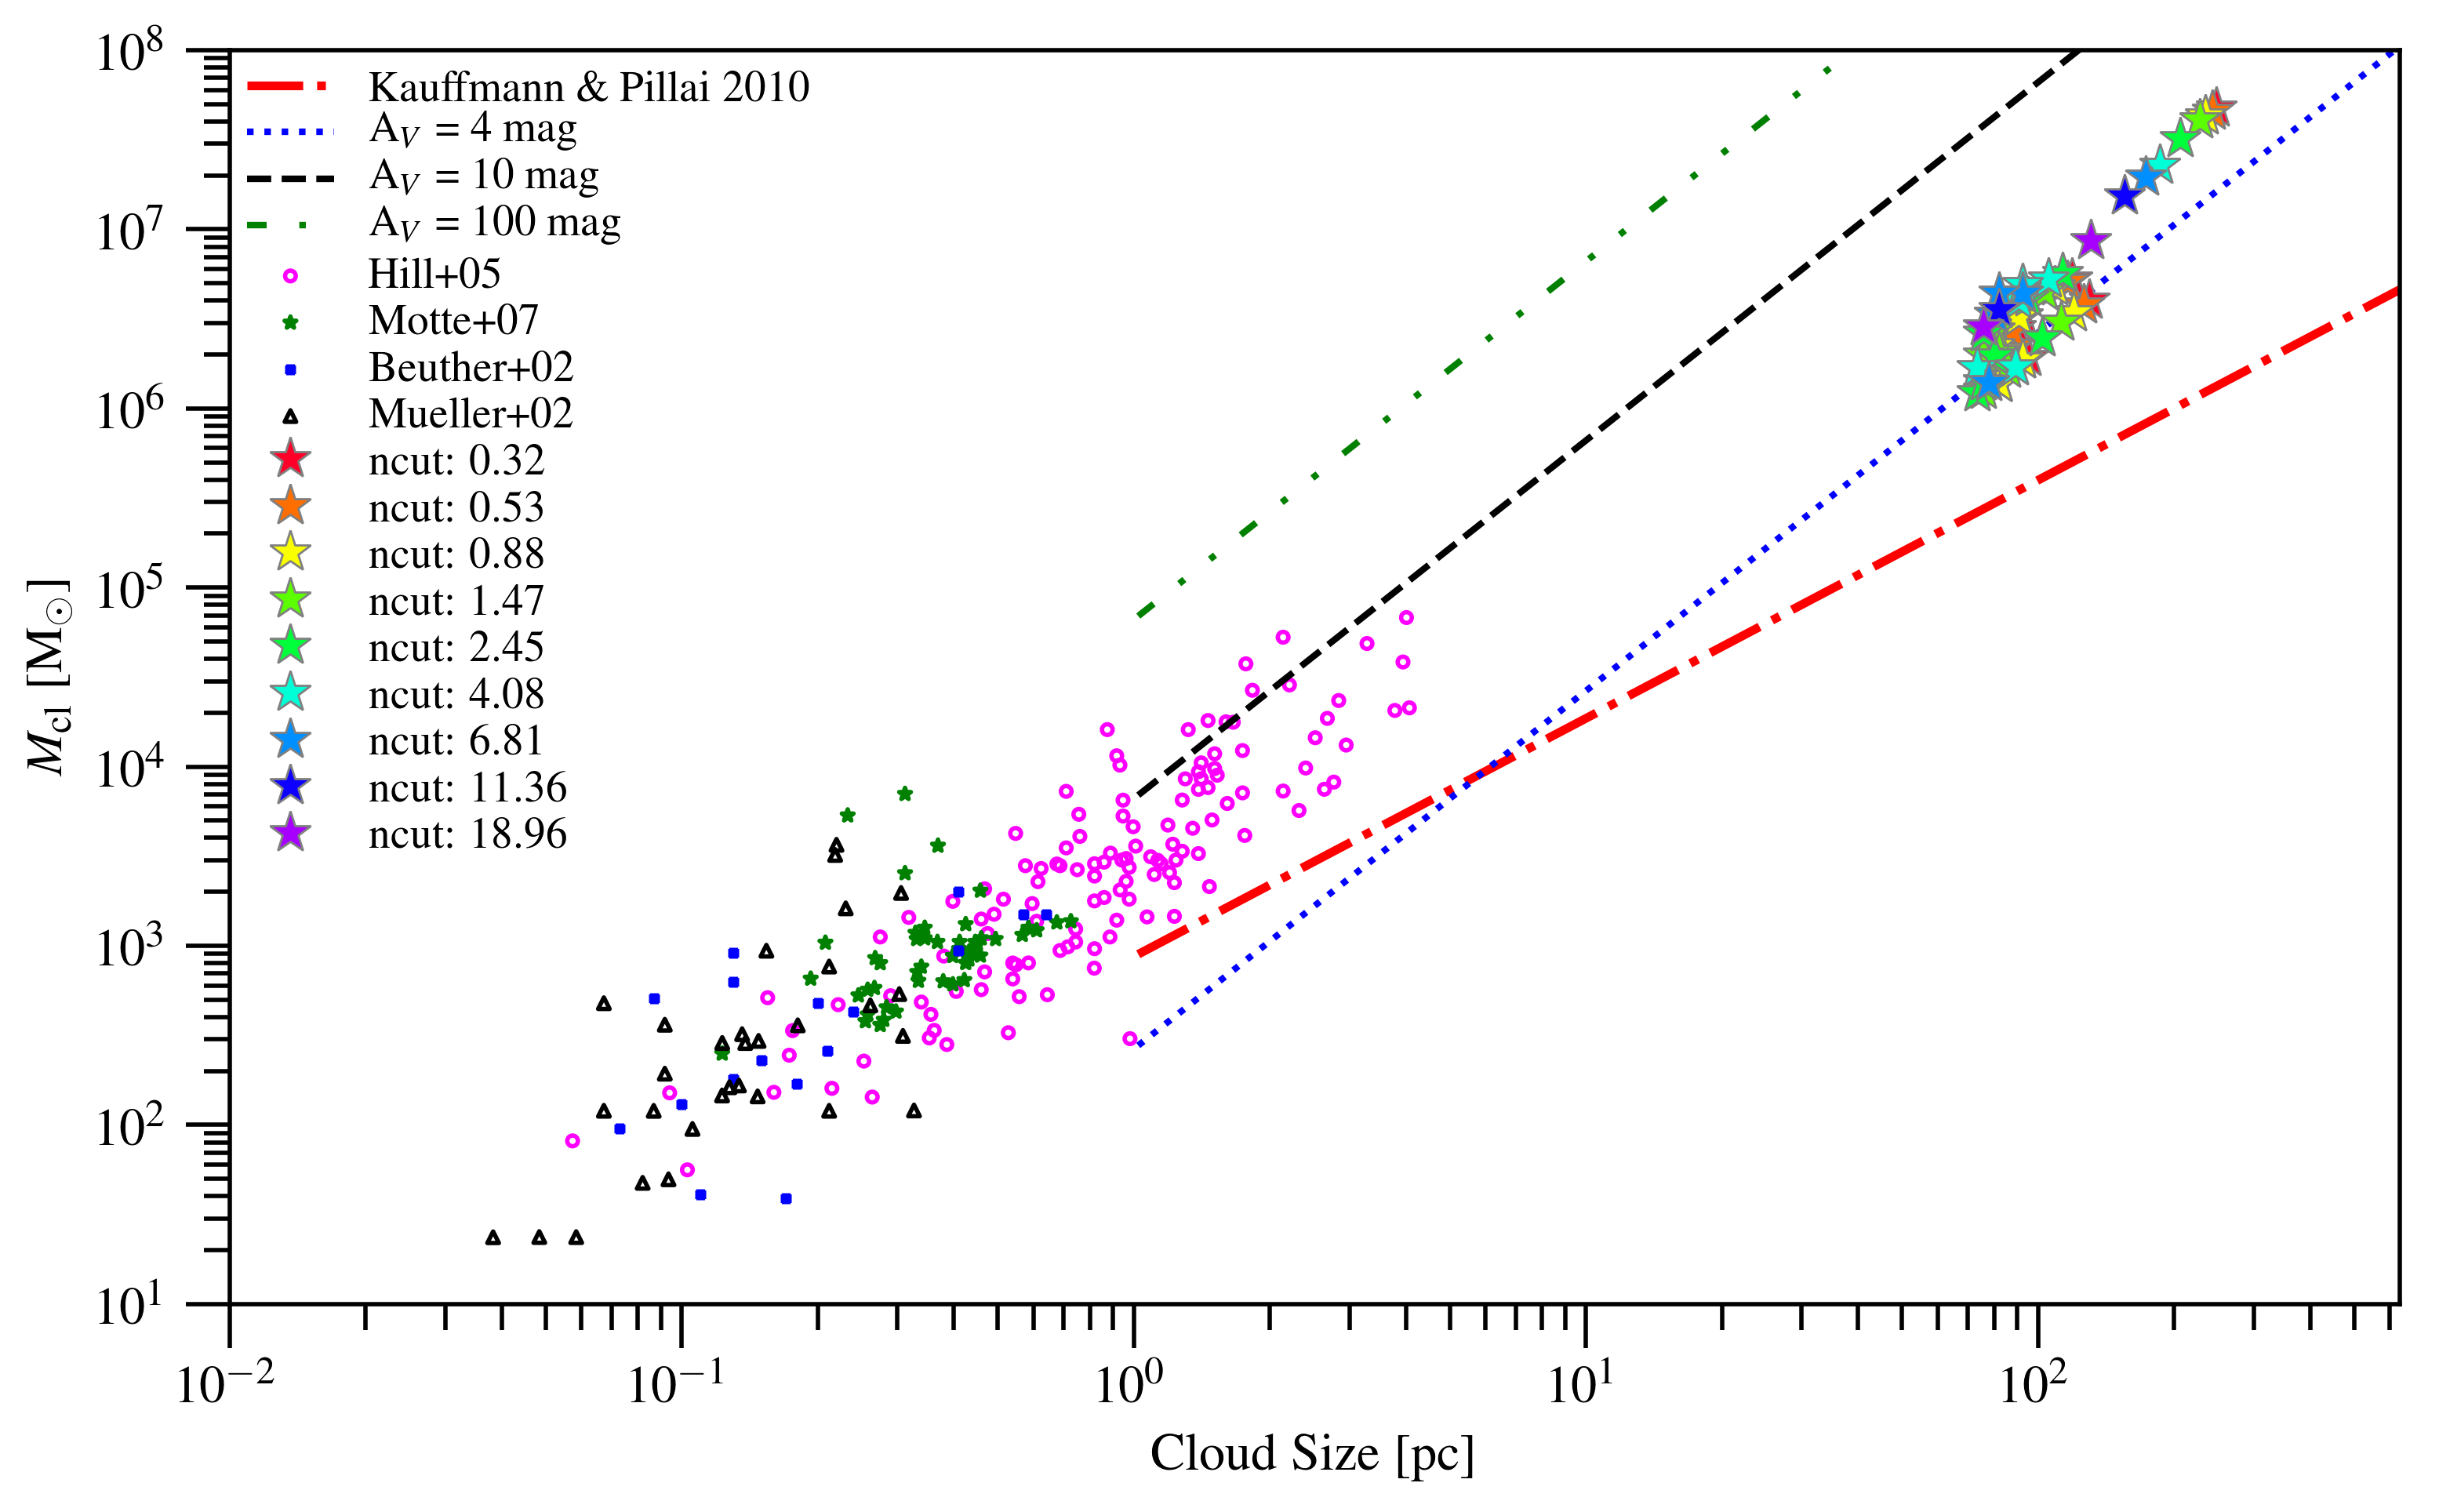
\includegraphics[trim=0 0 0 0, clip, width=0.8\textwidth]{\figpath/lf16_cloud-mass_size-pc.png}
\caption{
Size-mass relation of MCs identified in the accretion phase of \flower in our simulation (star symbols)
compared to observational data of molecular clouds in the Milky Way associated with massive \SF
(magenta circles, green stars, blue dots, and black triangles) and empirical relations
established based on \obs of the Milky Way.
Red line shows the threshold for massive \SF reported by \citet{Kauffmann10b}.
Star symbols are color-coded by increasing $n_{\rm cut}$.
Literature data are compiled from \citet{Beuther02a, Mueller02a, Hill05a, Motte07a}.
The colored lines show the loci expected for various visual extinctions ($A_V$), which corresponds to
lines of constant surface density (i.e., Larson's third relation). This representation is motivated by observational studies (see text and e.g., \citealt{Lombardi10a}).
\label{fig:MR}}
\end{figure*}

Maps of the gas Toomre $Q$ parameter and the effective two-component $Q_{\rm eff}$ parameter along different projection angles during the accretion phase of \flower are shown in \Fig{Q} and \Fig{Qeff}, respectively (see \Fig{h2density} for examples of clumps identified 
in this snapshot). Fragmentation are expected in regions of low Toomre Q values.
Further interpretation and implication of this is discussed in \Sec{origin}.


\begin{figure*}[htbp]
\centering
\includegraphics[trim=0 20 30 30, clip, width=0.85\textwidth]{\figpath/ss_16_toomre_proj_0}
\caption{
Maps of the total gas surface density (top left), 
velocity dispersion (top right),
epicyclic frequency (bottom left), 
and Toomre $Q$ parameter (bottom right) in the $xy$-plane.
Modest smoothing has been applied to the maps. 
A divergent colormap is used for the Toomre $Q$ map to facilitate 
identification of regions above and below $\log{Q_{\rm gas}}$\eq0.
\label{fig:Q}}
\addtocounter{figure}{-1}
\end{figure*}

\begin{figure*}[htbp]
\centering
\includegraphics[trim=0 20 30 30, clip, width=0.85\textwidth]{\figpath/ss_16_toomre_proj_1}
\caption{Continued. Maps showing the various quantities projected in the $xz$-plane.}
\addtocounter{figure}{-1}
\end{figure*}

\begin{figure*}[htbp]
\centering
\includegraphics[trim=0 20 30 30, clip, width=0.85\textwidth]{\figpath/ss_16_toomre_proj_2}
\caption{Continued. Maps show the various quantities projected in the $yz$-plane.}
\end{figure*}





%--------------------------------------------------------------------------
%                                Discussion
%--------------------------------------------------------------------------
\section{Discussions and Implications}     \label{sec:diss}

\subsection{Placing Results in the Context of Existing Observations} \label{sec:diss1}

The population of sub-MCs has dynamics largely
similar to those observed
in $z$\ssim2 spatially resolved studies of gas-rich star-forming galaxies, in
terms of their velocity dispersions, sizes, and gas surface densities (\Fig{larsons_single}; see
e.g., \citealt{Swinbank11a}), with sizes of the order of $R\simeq$\,100\,pc and velocity
dispersions of $\sigma\simeq$\,20$-$80\,\kms.
% velocity dispersion, larsons
Their velocity dispersions are also comparable to those observed in the inner Milky way and
nearby gas-rich galaxies (e.g., M64; \citealt{Oka01a, Rosolowsky05a, Heyer09a}), which lies
along the locus of $\sigma\propto R^{0.56}$.
Such high velocity dispersions and surface densities are expected since
they are located in the nuclear regions of the
galaxy, where the potential well is also deeper. The higher velocity dispersions (see also 
footnote~\ref{ftn:veldisp} on page \pageref{ftn:veldisp})
of these MCs can also be understood as they have experienced more recent episodes
of \SF as \flower is assembling its stellar mass (these MCs also have higher stellar-to-gas mass ratios of $\sim$60).
In fact, by $z\simeq$\,7.2 (i.e., the snapshot corresponding to an early phase of accretion as
shown in \Fig{SFH}a), \flower has assembled
a stellar mass of $M_*$\eq7.5\E{9}\,\Msun. Thus, the higher velocity dispersion
is due in part to the stronger stellar feedback compared to e.g., MCs in its satellite galaxies ($\sigma\approx$10\,\kms).

The high pressure observed in \flower is comparable to what has been 
observed in local ultra-luminous IR galaxies (ULIRGs); however, the
molecular clouds in the latter are concentrated within their 
central regions and have typical sizes of $\sim$70-100\,pc and masses on the order of $\sim$10$^9$\,\Msun
\citep{Downes98a, Sakamoto08a}. In our simulation, the high pressure MCs of \flower are
found throughout the disk. This difference likely stems from the different physical mechanisms giving rise
to the formation (and thus the nature) of these molecular structures.
For instance, in local ULIRGs, they are likely form by shock compression and cloud-cloud
collision after large amount of gas from the pair of progenitor galaxies
are being funneled toward the central region \citep{Tan00a, Wu18a}.  % Tasker09a
On the other hand, the highly turbulent structures of \flower likely result from 
constant cold gas accretion onto the entire galaxy (without
requiring gas to be funneled into the central region).
This latter mechanism may also be the dominant mode for forming the highly supersonic massive MCs observed
in gas-rich star-forming galaxies at $z$\ssim2 (see also e.g., \citealt{Swinbank11a}) --- but the observed 
size scales could also result from resolution limit where the true physical scales of MCs in
$z$\,\ssim2 galaxies could be smaller in reality.
The constant inter-cloud collision as gas is being accreted onto the main galaxy would also render
the MCs to be gravitationally unbound (see e.g., \citealt{Dobbs11a}), which is 
consistent with the high $\alpha_{\rm vir}$ found for the MCs in the main disk of \flower.

% mass-size relation
In terms of the mass-size relation (\Fig{MR}), the MCs of \flower are found to lie above the \citet{Kauffmann10c} relation, 
which is an empirical relation corresponding to the threshold for massive \SF, but lies
%The implication of this \citet{Kauffmann10c} relation is that cluster-forming cloud fragments are
%found to be more massive than those that are devoid of clusters
%at a given radius.
below the locus of $A_V$\eq100\,mag followed by Milky Way clouds.
This can be understood by acknowledging the fact that a H$_2$ molecular cloud
does not necessary contain CO (e.g., as CO forms deeper in molecular clouds),
and that our simulation does not have enough resolution to directly form CO\footnote{
In fact, to form CO and make predictions for CO line emission in the work presented by \citet{Vallini18a}, we
model the internal structure of MC within each cell in our simulation.}.
That is, the MCs of \flower lying along the locus of $A_V$\eq4\,mag likely manifests from the
fact that the MCs in our simulation have lower column densities than the star-forming cores observed in the Milky Way, which are
observationally well-resolved within an MC, and indeed, have sufficient column density to form CO.


% different evolutionary stages
In the scaling relations examined, we find similar MC properties 
in relation to those observed in the nearby Universe between the accretion phase and the starburst phase of
\flower (see \Fig{larsons_single}, \Fig{alpha16}, and \Fig{alpha27}).
That is, we do not find any quantitative major differences in the MC properties between the accretion and the starburst phase, which
are separated by $\simeq$300\,Myr.

 
\subsection{Origin and Physical Scales of the MCs} \label{sec:origin} 
The largest molecular structure identified is essentially the main disk of \flower and breaks down into smaller
substructures that are denser as we increase $n_{\rm cut}$ (see e.g., \Fig{larsons16-28}). Overall,
the MCs we identified are much bigger in size and mass than nearby GMCs, 
but comparable to those observed in $z$\,\ssim2$-$4 galaxies based on spatially resolved imaging \citep{Swinbank11a}.

% mass scale
Observations of nearby gas-rich galaxies such as M64 and NGC\,253
show higher velocity dispersions compared
to the disk/mid-plane of the Milky Way but consistent with those observed in the inner regions of
Milky Way and M51 \citep{Oka01a, Rosolowsky05a, Heyer09a, Hughes13b, Leroy15a, Rice16a}.  % also higher $P_{\rm int}$,
% which is $\propto\rho\sigma^2$
% M51: Colombo+14
However, clouds in nearby gas-rich galaxies are bigger in size (approximately
an order of magnitude) and mass (approximately two orders of magnitude).
These bigger clouds have been interpreted as a results of their 
higher gas mass fractions and
surface densities and velocity dispersions, since
fragmentation occurs near the Jeans length $L_J\propto\sigma^2/\Sigma$
and Jeans mass $M_J\propto\sigma^4/\Sigma$
for dispersion-supported structures.

Based on the scaling of $M_J$\eq$\sigma^4/(G^2\Sigma)$ for the Jeans mass,
a velocity dispersion of $\sigma\approx50$\,\kms and a gas mass surface density of
$\Sigma_{\rm gas}\approx450$\,\Msun\,pc$^{-2}$
yield $M_J\sim$\,8\E{8}\,\Msun, which is in good agreement with the mass range found in the MCs identified (see \Fig{dist}).
Similarly massive molecular clouds have been reported in idealized closed-box isolated galaxy
simulations done at higher resolution (e.g., \citealt{Behrendt16a}).
Note, however, that the IGM and merger and accretion histories are not properly modeled in such simulations
since they adopt non-cosmological initial conditions.
That said, this is reassuring --- our results are not far off in spite of the resolution ($l\approx$\,30\,pc).

%Note that regions of $Q\lesssim1$ is actually somewhat 
%less than the number of MCs we have identified based on density threshold --- 
%but this has something to do with the dependence on 
%$n_{\rm cut}$. The number of MCs and regions of low $Q$ are comparable if we only look at 
%MCs identified at the highest $n_{\rm cut}$. \DL{do they overlap?}

% alpha parameters
As shown in \Fig{alpha16}, the virial parameter of the sub-MCs is about $\alpha_{\rm vir}\gtrsim10$, which 
is considerably lower than their ``parent'' MCs found in the main disk of \flower ($\alpha_{\rm vir}\gtrsim100$).
For the MCs in the satellite galaxies, a lower virial parameter is found 
compared to the (sub-)MCs in the main disk of \flower, with $\alpha_{\rm vir}\approx$\,2.
Differences in their $\alpha_{\rm vir}$ most likely result from the weaker
stellar feedback in the satellite galaxies as they have experienced less episodes of \SF compared to
\flower (i.e., lower stellar-to-gas mass ratios of $\sim$0.1).
% pext
As shown in \Fig{alpha27}, MCs in the main disk of \flower have higher pressure than the sub-MCs.
The lower virial parameter and external pressure of the sub-MCs
compared to their parent MCs are consistent with
the notion that collapsing structures result from local gravitational
instability within globally non-collapsing structures \citep[see e.g.,][]{Ballesteros-Paredes11a},
which are supported by turbulence and rotation on large scales.
%Based on the virial parameter, velocity dispersion, and pressure of the MC identified in the main disk of \flower,
%the MC itself is gravitationally unbound and supported by turbulence (from the feedback of multiple episodes of \SF)
%and galactic rotation on large scales. 
%% Turbulence in these substructures further dissipates in % e.g., shocks on even smaller scales, allowing sub-MCs to be bound and collapse.

For MCs in the satellite galaxies, we find low pressures and virial parameters 
which are comparable to those found in clouds formed in the galactic disks 
($\alpha_{\rm vir}$\eq0.2$-$10; \citealt{Dobbs08a, Tasker09a}).
This suggests that MCs identified in the satellite galaxies are likely to be collapsing structures,
and thus, \SF is expected to continue 
as gas from satellite galaxies is being accreted onto the main galaxies during the EoR.

The apparently large virial parameters seen in the MCs of \flower can be understood using the 
Toomre $Q$ parameter (\Fig{Q} and \Fig{Qeff}). 
We first note that fragmentation {\it can} happen in regions of low $Q$ (if we only consider 
instability against axisymmetric perturbations), but  
further evolution/collapse depends on the dynamics or equation of state of the gas. 
Such fragmentation is expected to take place at the
critical scale length $\lambda_{\rm crit} < 2 \pi^2 G \Sigma / \kappa^2$.
Second, this fragmentation scale is greater than the typical size of GMCs. This could be interpreted as a result of instability setting the scales for fragmentation, but the star-forming GMCs
correspond to the collapsing, denser, and cooler molecular structures that are on smaller scales. 
Thus, the high virial parameter found 
for most MCs in \flower, which is the ratio between the velocity dispersion (accounts for effect of pressure 
and rotation) and surface density, indicate that most of them are not collapsing structures. 
As such, some MCs lie in regions of $Q>1$. 
Only in (the denser) regions with a low Toomre $Q$ parameter and 
when energy can be dissipated on a timescale 
that is shorter than the timescale over which it gains energy (e.g., heating) 
correspond to star-forming {\it clumps} and {\it cores} with low virial parameters.
This would also (at least partially) explain the seemingly inconsistency between the high $\alpha_{\rm vir}$
nature of most MCs of \flower and its relatively high SFR.
That is, if most of the molecular gas in \flower are stable against collapse, 
how does it sustain its high SFR of $\sim$100\,\Msun\,yr\pmOne?
The discrepancy can be explained in two ways.
First, our results are limited by the resolution of the simulation, such that, in each MC, there
likely exist multiple smaller-scales molecular structures (e.g., clumps and cores),
as in the classical molecular cloud hierarchy. This re-iterates the statement about low $Q$ above.
Second, due to turbulence dissipation on small-scales, such (sub-)structures are no longer supported by
large-scale gravitational potential and differential rotation.
This in turn enables subregions of the MCs to collapse and potentially form OB associations out of these unbound
MCs \citep{Clark04a, Clark05a}.
Additional mechanisms causing non-axisymmetric perturbations (e.g., arms) to the gravitational potential
can also induce orbit crossing, shocks and dissipation in gas, further promoting turbulence dissipation
and collapse on smaller scales to trigger \SF.

%--------------------------------------------------------------------------
%                                Conclusions
%--------------------------------------------------------------------------
\section{Summary and Conclusions}      \label{sec:conclusion}

We study the dynamical properties of molecular clouds complexes and their temporal evolution in a \z$\sim$\,6 prototypical galaxy
at the EoR using state-of-the-art cosmological zoom-in simulation (\ncode{Serra}),
which includes a chemical network to determine the formation of molecular
hydrogen, heating and cooling of the ISM by metals, and stellar feedback.
We use a clump-finding algorithm and a set of H$_2$ volumetric densities
to identify MCs and their sub-structures in the main galaxy of the
simulated 20\,Mpc~$h$\pmOne box --- \flower\ --- and in its satellites.
We decompose the molecular structures into non-overlapping tiles
by identifying a set of different density contours at different snapshots.
Using volumetric H$_2$ is essentially similar to identifying molecular structures using
different contour levels/surfaces on surface brightness maps/cubes of molecular line tracers (e.g., CO, CS, NH$_3$),
since the line luminosity scales with the molecular gas density (modulo optical depth effects).
We extract properties such as mass, size, Mach number, velocity dispersion, gas surface density, and virial parameter for each MC and
compare them with those observed in the Milky Way disk, the Galactic center,
and gas-rich starburst galaxies in the local Universe and at the peak epoch of cosmic \SF.
We also examine their properties at the different evolutionary stages of \flower and compare
them with observations.

We find that the MC of \flower are highly supersonic, with high velocity dispersions ($\sigma\approx$\,200\,\kms) comparable to
those observed in $z$\ssim2 starburst galaxies.
The mass scale of the MCs is of the order of $10^{6.5-9}$\,\Msun. The $\sim$200\,pc-scale MCs found with a low density threshold
correspond to the arms of the disk of \flower which break down into smaller $\lesssim$100\,pc-scale MCs at higher density thresholds.
The more massive and bigger MCs in \flower compared to the Milky Way
likely result from the higher gas mass fraction, surface density, and velocity dispersion,
which set the scale for fragmentation.
This is consistent with what has been found previously in higher resolution idealized simulation of isolated galaxies.
Our simulation here confirms these results at EoR and under
the influence of continuous gas accretion from the surrounding IGM (see e.g., \citealt{Klessen10a, Goldbaum11a}).

We compare the dynamics of MCs in \flower to \obs in the context of the Larson's relation.
The MCs of \flower are found to have higher $\sigma$ and $\Sigma$ systematically regardless of the 
density threshold $n_{\rm cut}$ adopted in identifying the structures.
Our results are thus insensitive to the various density cuts of choice.
%However, our results are dependent on the numerical resolution of the simulation.
The velocity dispersion remains $\gtrsim$100\,\kms even when we increase the 
density threshold and even for the molecular substructures.
Such a high velocity dispersion likely results from
the strong supernova and stellar feedback \flower experienced over the multiple episodes of bursty \SF.

Virial analysis indicates that the MC/arms of the main disk of \flower are unbound, but the substructures have lower virial parameter.
This is consistent with the notion that collapsing structures result from gravitational instability within globally stable structures, which are
supported by turbulence and rotation on large scale.
We also find $\alpha_{\rm vir}\approx$\,2 for the MCs in the satellite galaxies, which we interpret as
result of the weaker stellar feedback as they have
experienced less episodes of \SF compared to \flower (also supported by the lower stellar-to-gas mass ratio of the latter).
MCs in the satellites are therefore likely collapsing structures.

We find no temporal variations in the MC dynamics over the course of 700\,Myr traced in our simulation, 
at least in terms of the scaling relations examined.
Our results are robust against the H$_2$ volume density threshold adopted (see Appendix \Sec{ncut}).

Determining the multi-phase ISM properties of early galaxies
is a critical piece to understanding the evolution and
assembly history of galaxies, since they set the pace
for chemical reactions and excitation rates for the coolants in the ISM (and subsequent star formation).
Observations leveraging the combination of spatial-spectral imaging of
multi-band continuum and spectral line emission are crucial for better understanding
the role of \highz galaxy populations
in the context of galaxy evolution and the ISM physics behind their intense star formation in the early Universe.
Cosmological zoom-in simulations, such as \ncode{Serra}, while inherently limited in galaxy
statistics and is subject to the sub-grid models adopted, 
serve as an useful avenue/tool for examining and making predictions on the morphology and dynamics of
the multi-phase ISM structures of the first galaxies.
These predictions can in turn be
tested with high resolution imaging of the gas content in the first galaxies with telescopes such as ALMA and the ngVLA,
enabling us to test our findings and refine future simulations to shed light on the physical processes behind 
\SF since the cosmic dark ages.


%==============================================================================
%                                Back matters
%==============================================================================
% ACKNOWLEDGEMENTS
%-------------------------------------
\acknowledgements

We thank Jens Kauffmann, Thushara Pillai, and Mark Swinbank for sharing their data.
T.K.D.L. acknowledges support by the NSF through award SOSPA4-009
from the NRAO and support from the Simons Foundation.
A.F. acknowledges support from the ERC Advanced Grant INTERSTELLAR H2020/740120.
This work is based on a project developed at the Kavli Summer Program in Astrophysics (KSPA)
held at the Center for
Computational Astrophysics of the Flatiron Institute in 2018. The program was co-funded by the Kavli
Foundation and the Simons Foundation.
We thank the KSPA Scientific and Local Organizing Committees, and the program founder,
Pascale Garaud, for supporting the genesis of this work.
We also thank the Center for Cosmology and Particle Physics
at the New York University
for their hospitality in hosting us after the steam pipe explosion in NYC during the KSPA.
This research has made use of NASA's Astrophysics Data System Bibliographic Services
and \ncode{yt}, a community-developed Python package for analyzing simulation data in Astronomy.


\bibliographystyle{yahapj}
\bibliography{master_cleanup}

\appendix
\section{Variation in MC Properties Depending on the Choice of Density Cuts and
Temporal Evolution in Cloud Dynamics}    \label{sec:ncut}
% single Snapshot
We investigate possible variations in the dynamics of the molecular structures of \flower and its satellites
to test
the robustness of our results against the choice of density threshold by adopting
different sets of $n_{\rm cut}$ in identifying the MCs.
That is, how sensitive are the structure properties, and thus, the results presented in \Sec{singless}
dependent on the choice of density thresholds.
We vary the choice of H$_2$ density for each of the snapshots and
find no obvious differences in our results (i.e., inferences on the dynamics of \z$\sim$\,6
MCs in relation to those observed in nearby and \z$\sim$2 galaxies in the context of
cloud scaling relations).
In addition, for the densest MC in the main disk of \flower, we find that while
its size decreases as we increase $n_{\rm cut}$ --- as one would intuitively expect,
the velocity dispersion remain approximately $\sigma\simeq$\,200\,\kms (see also \Fig{larsons_single}).
This lack of variation is reassuring, in the sense that at least on the scales studied here,
the dynamics of the MCs are not artifacts or biased by our choice of $n_{\rm cut}$.
Our results are therefore robust to the various density cuts of choice.

% temporal evolution in Cloud Dynamics
We show the properties of all MCs identified across all snapshots
in \Fig{larsons16-28} and \Fig{alpha16-28}.
We find no quantitative differences in the cloud properties over the 700\,Myr traced in our simulation.

% -------------- all snapshots -----------


\begin{figure*}[htbp]
\centering
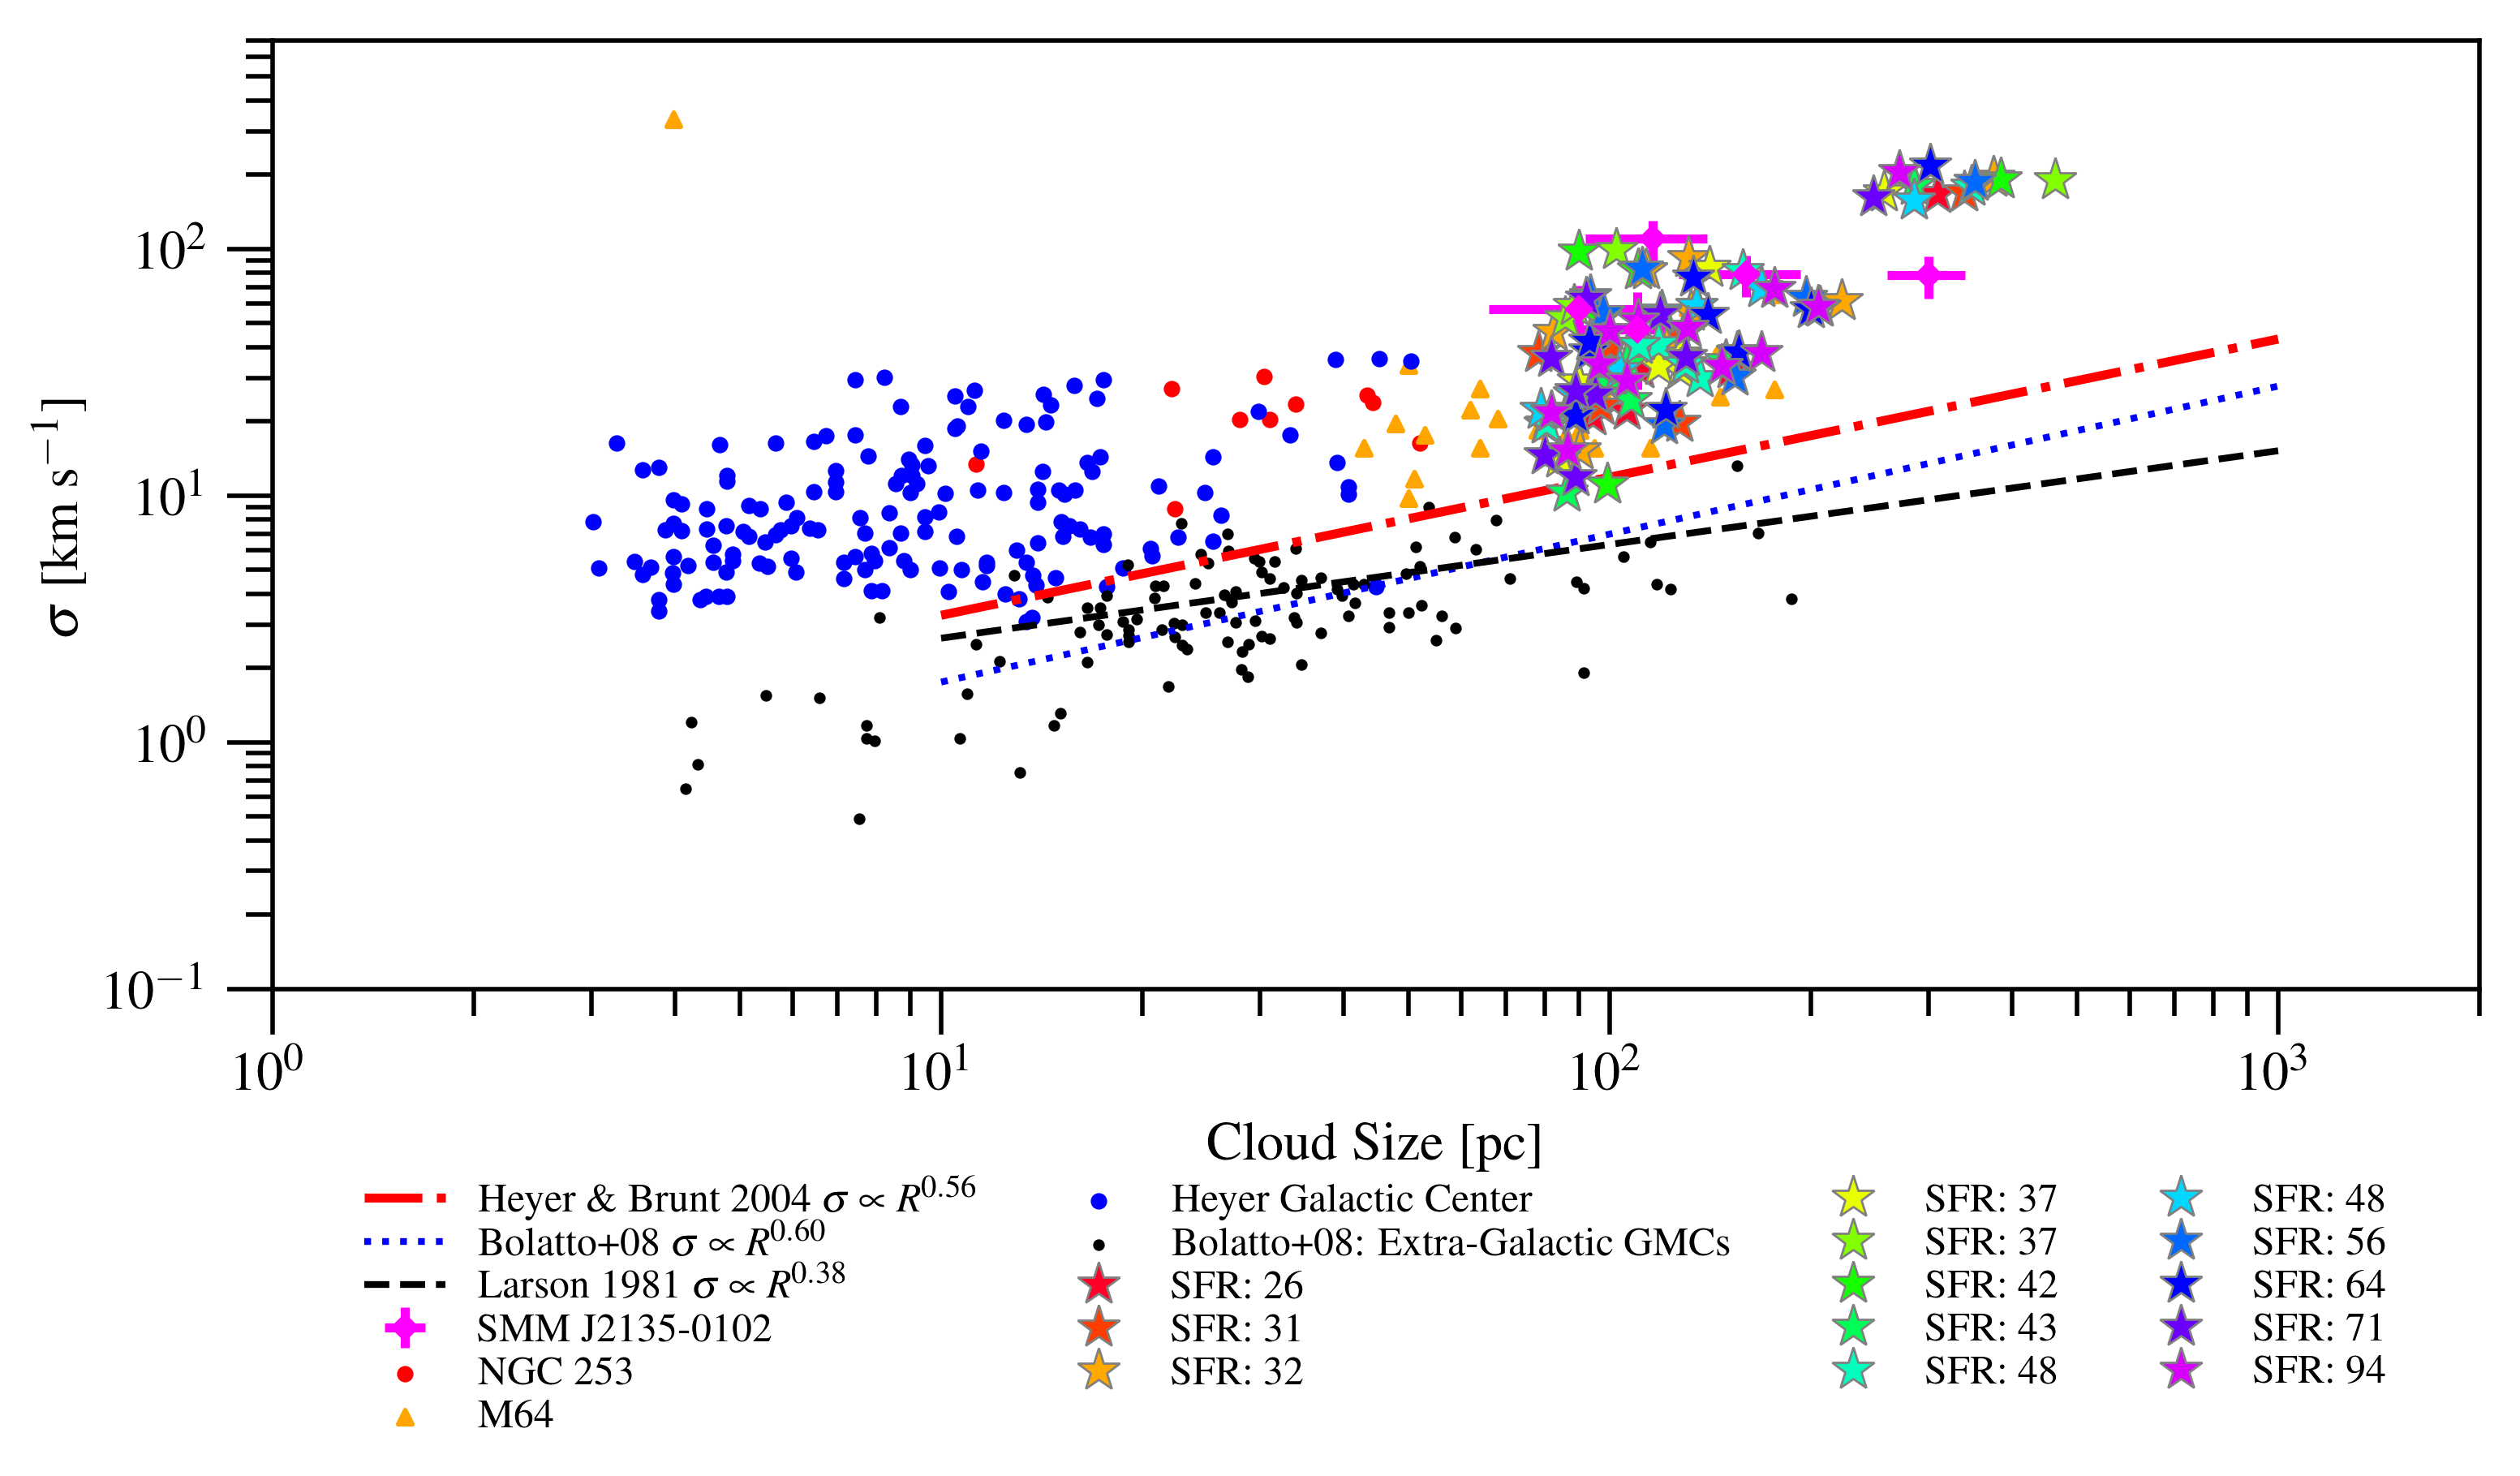
\includegraphics[trim=0 100 0 0, clip, width=0.85\textwidth]{\figpath/ss16-28_larsons.png}
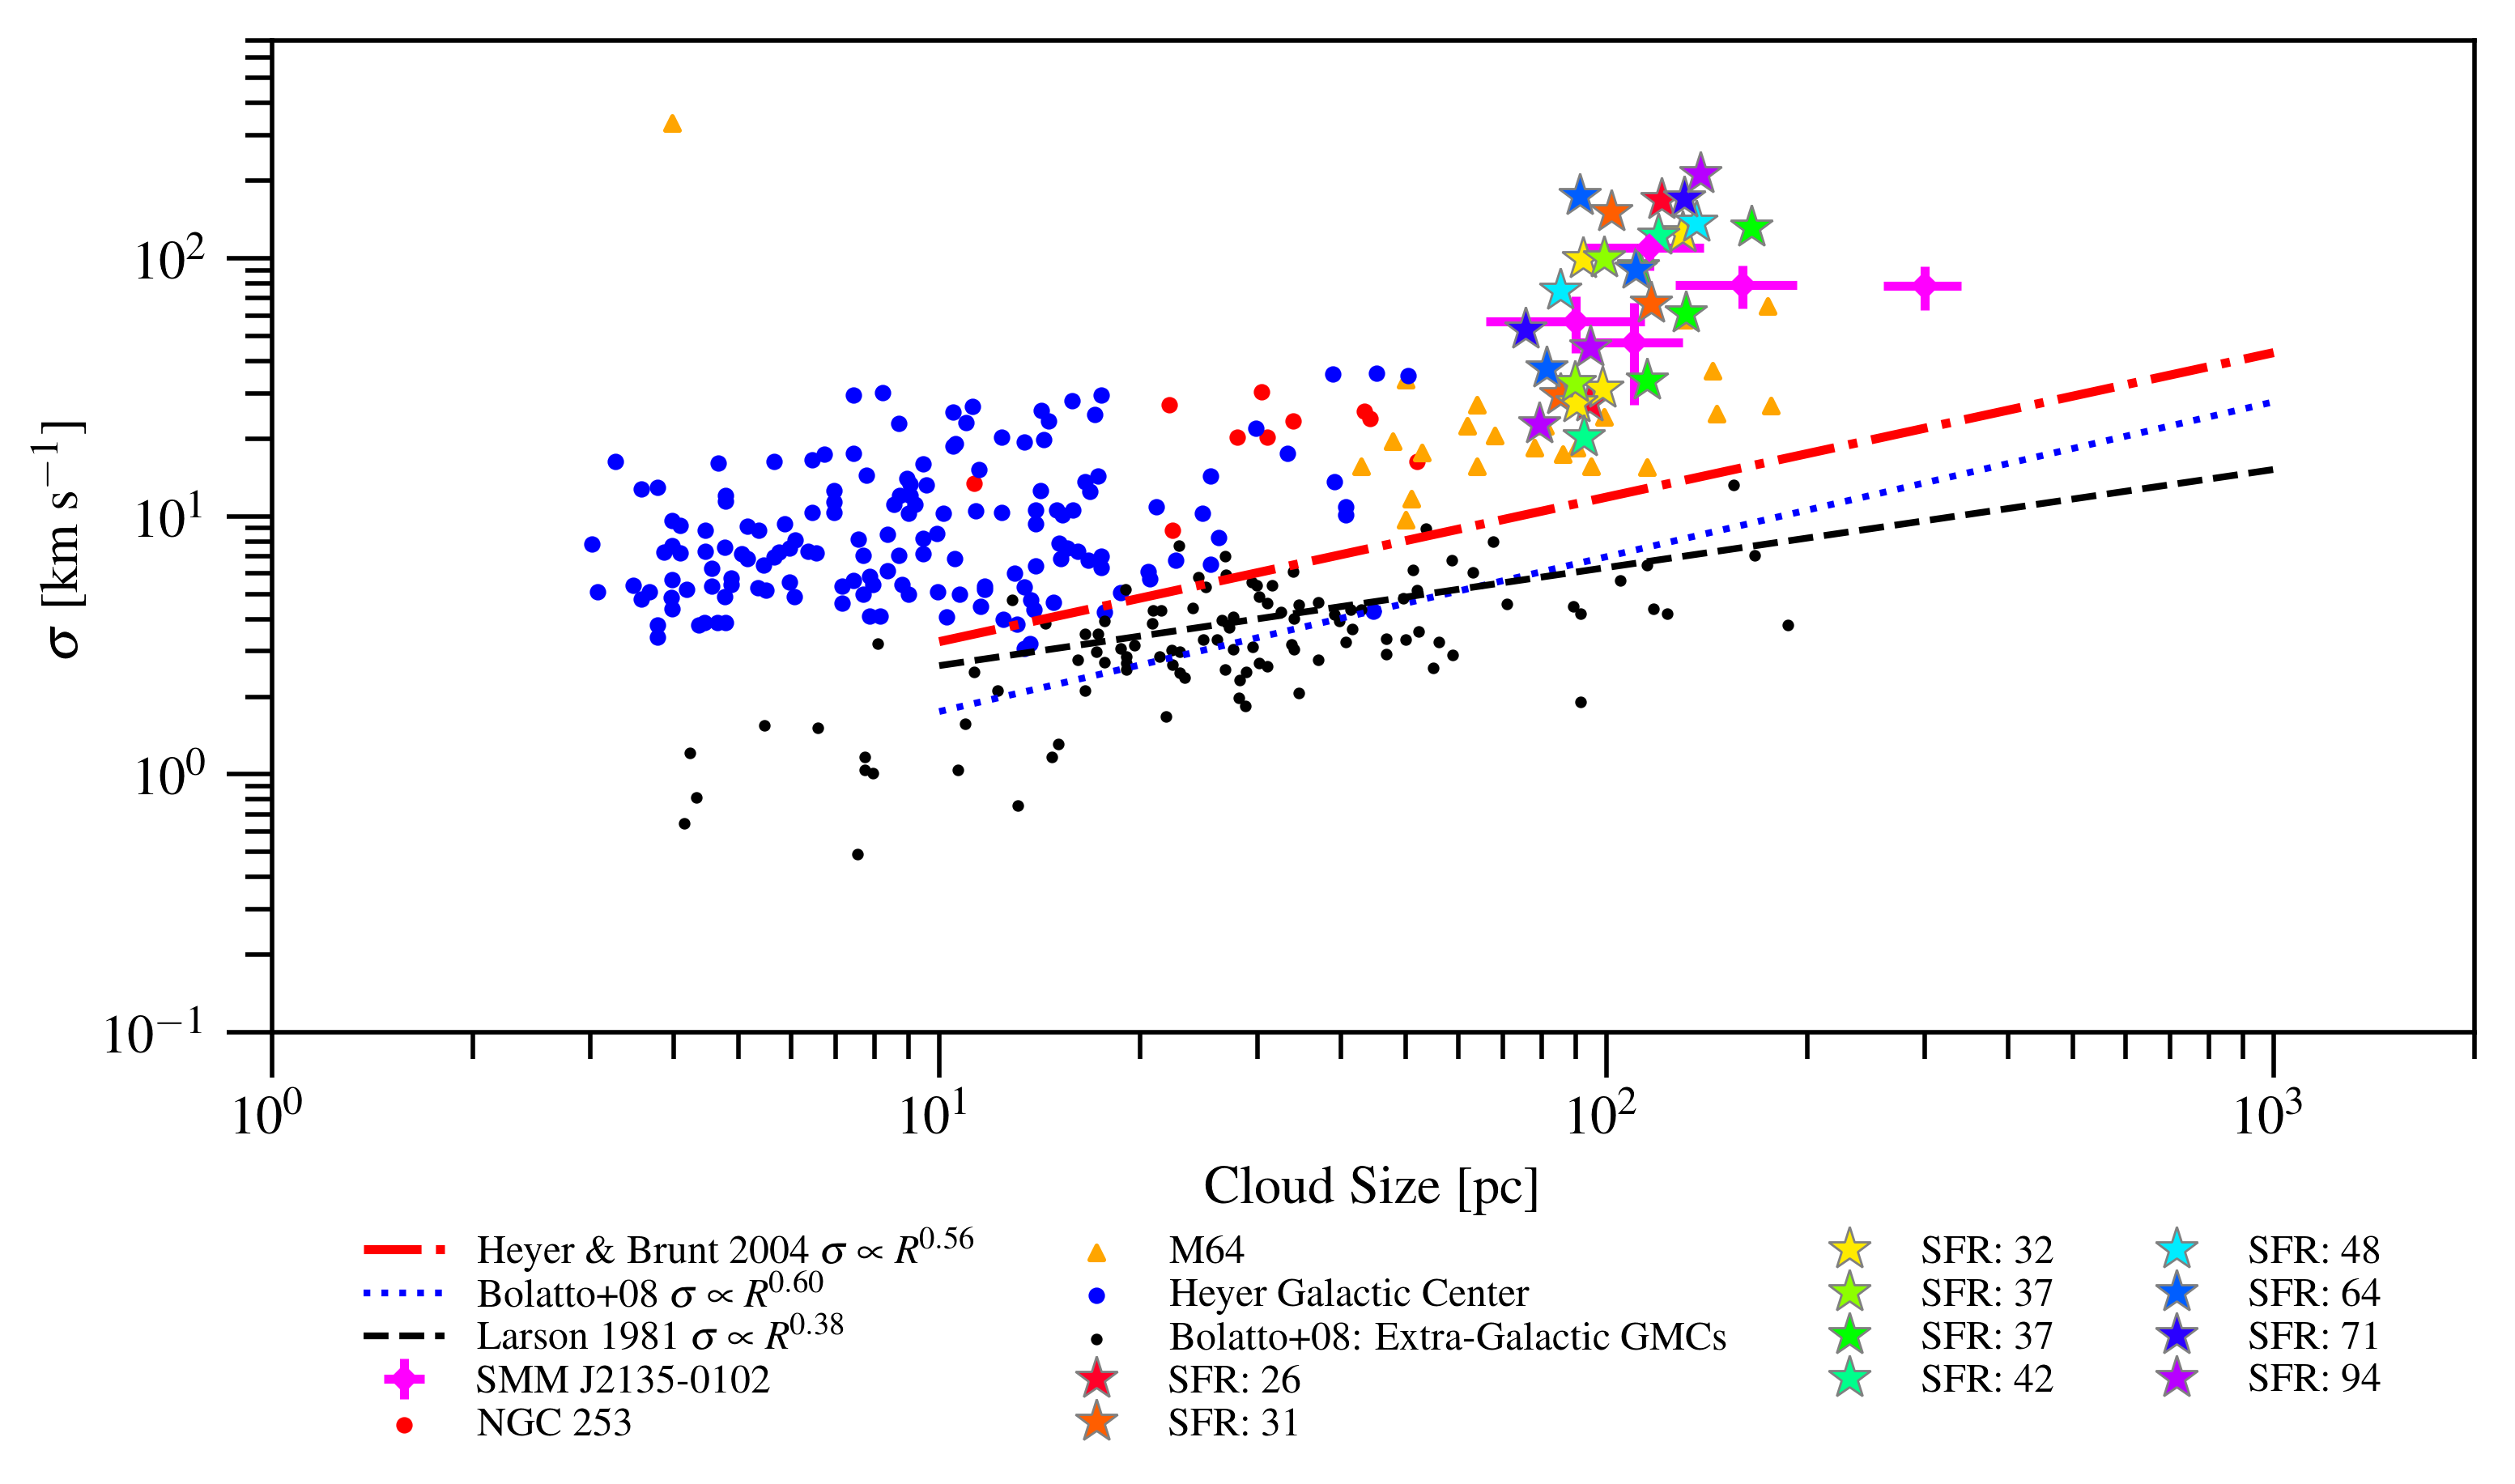
\includegraphics[trim=0 0 0 0, clip, width=0.85\textwidth]{\figpath/ss16-28-larsons-highncut.png}
\caption{
Comparison of MCs identified across all snapshots (over 700\,Myr; star symbols)
to those observed in nearby and \z$\sim$2 star-forming galaxies
in the context of the linewidth-size relation.
% showing variations in their properties at
% the different evolutionary phases of \flower and with varying SFRs.
Bottom panel corresponds to including only the denser substructures/sub-MCs identified in \flower
(i.e., MCs here are identified with the highest $n_{\rm cut}$, see \Sec{method}).
By and large, we find no quantitative differences in the mass-size relation over the 700\,Myr traced in the simulation.
\label{fig:larsons16-28}}
\end{figure*}

\begin{figure*}[htbp]
\centering
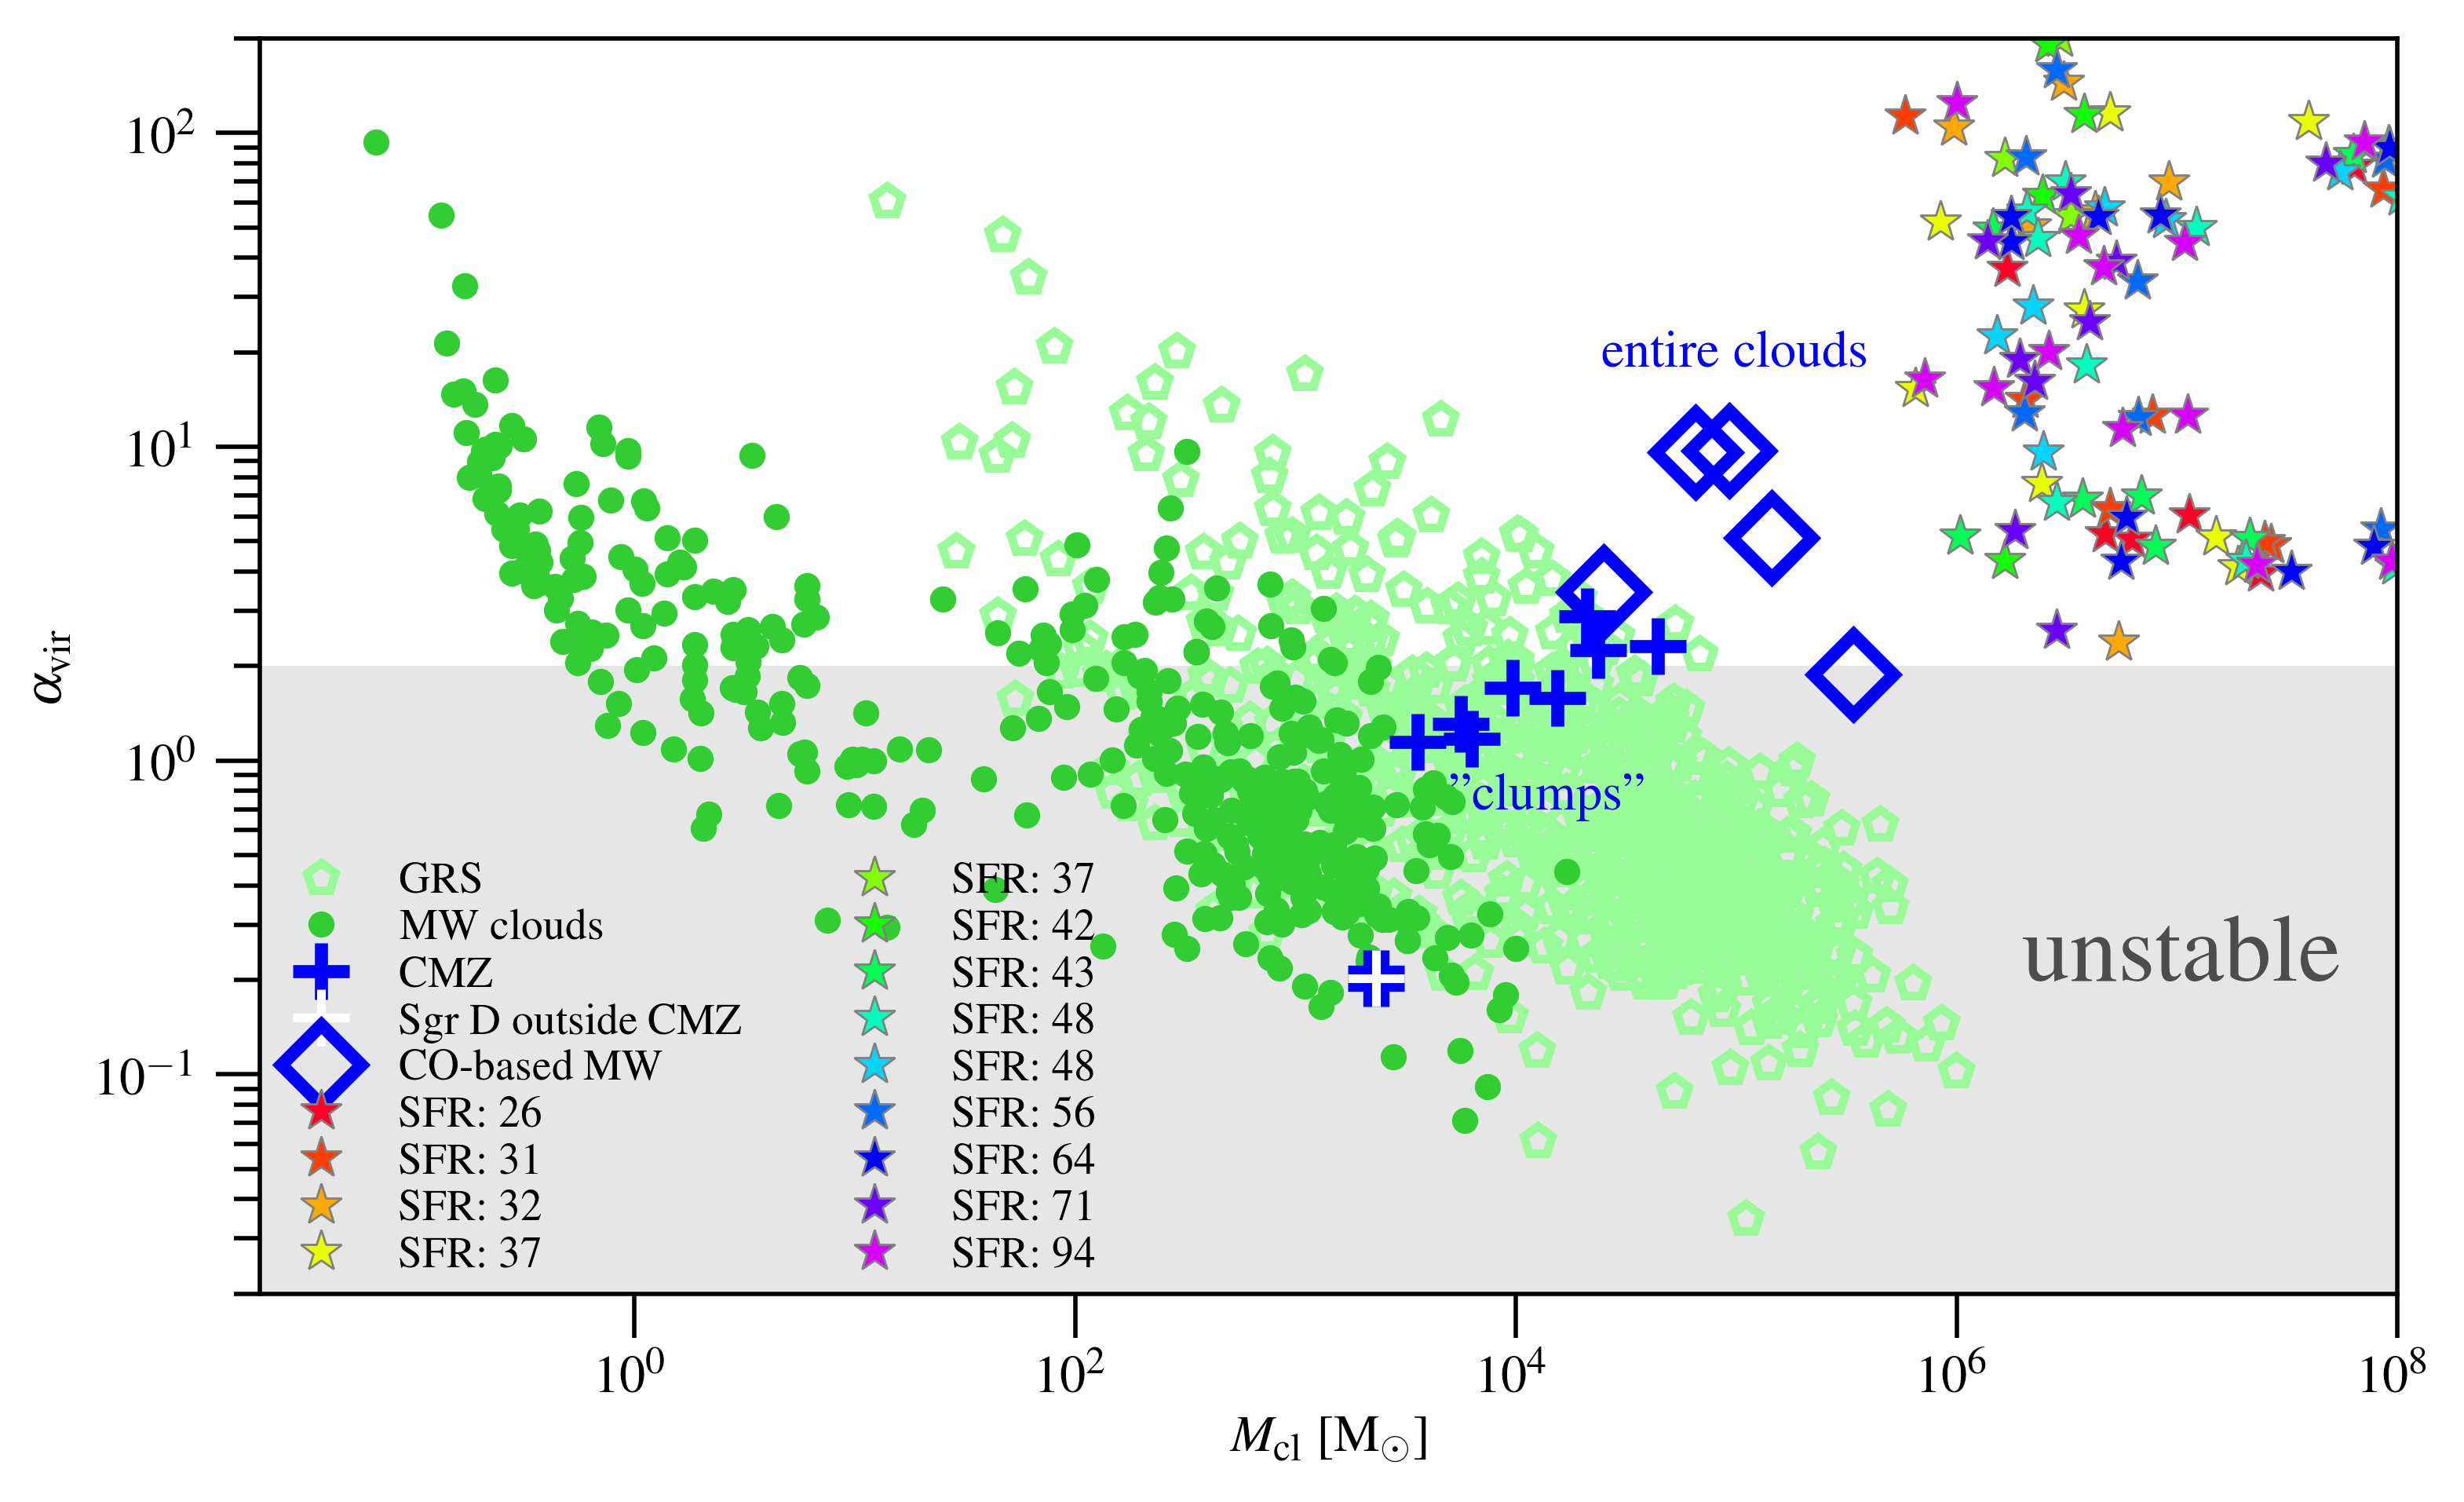
\includegraphics[trim=5 5 8 8, clip, width=0.515\textwidth]{\figpath/ss16-28_alphavir.png}
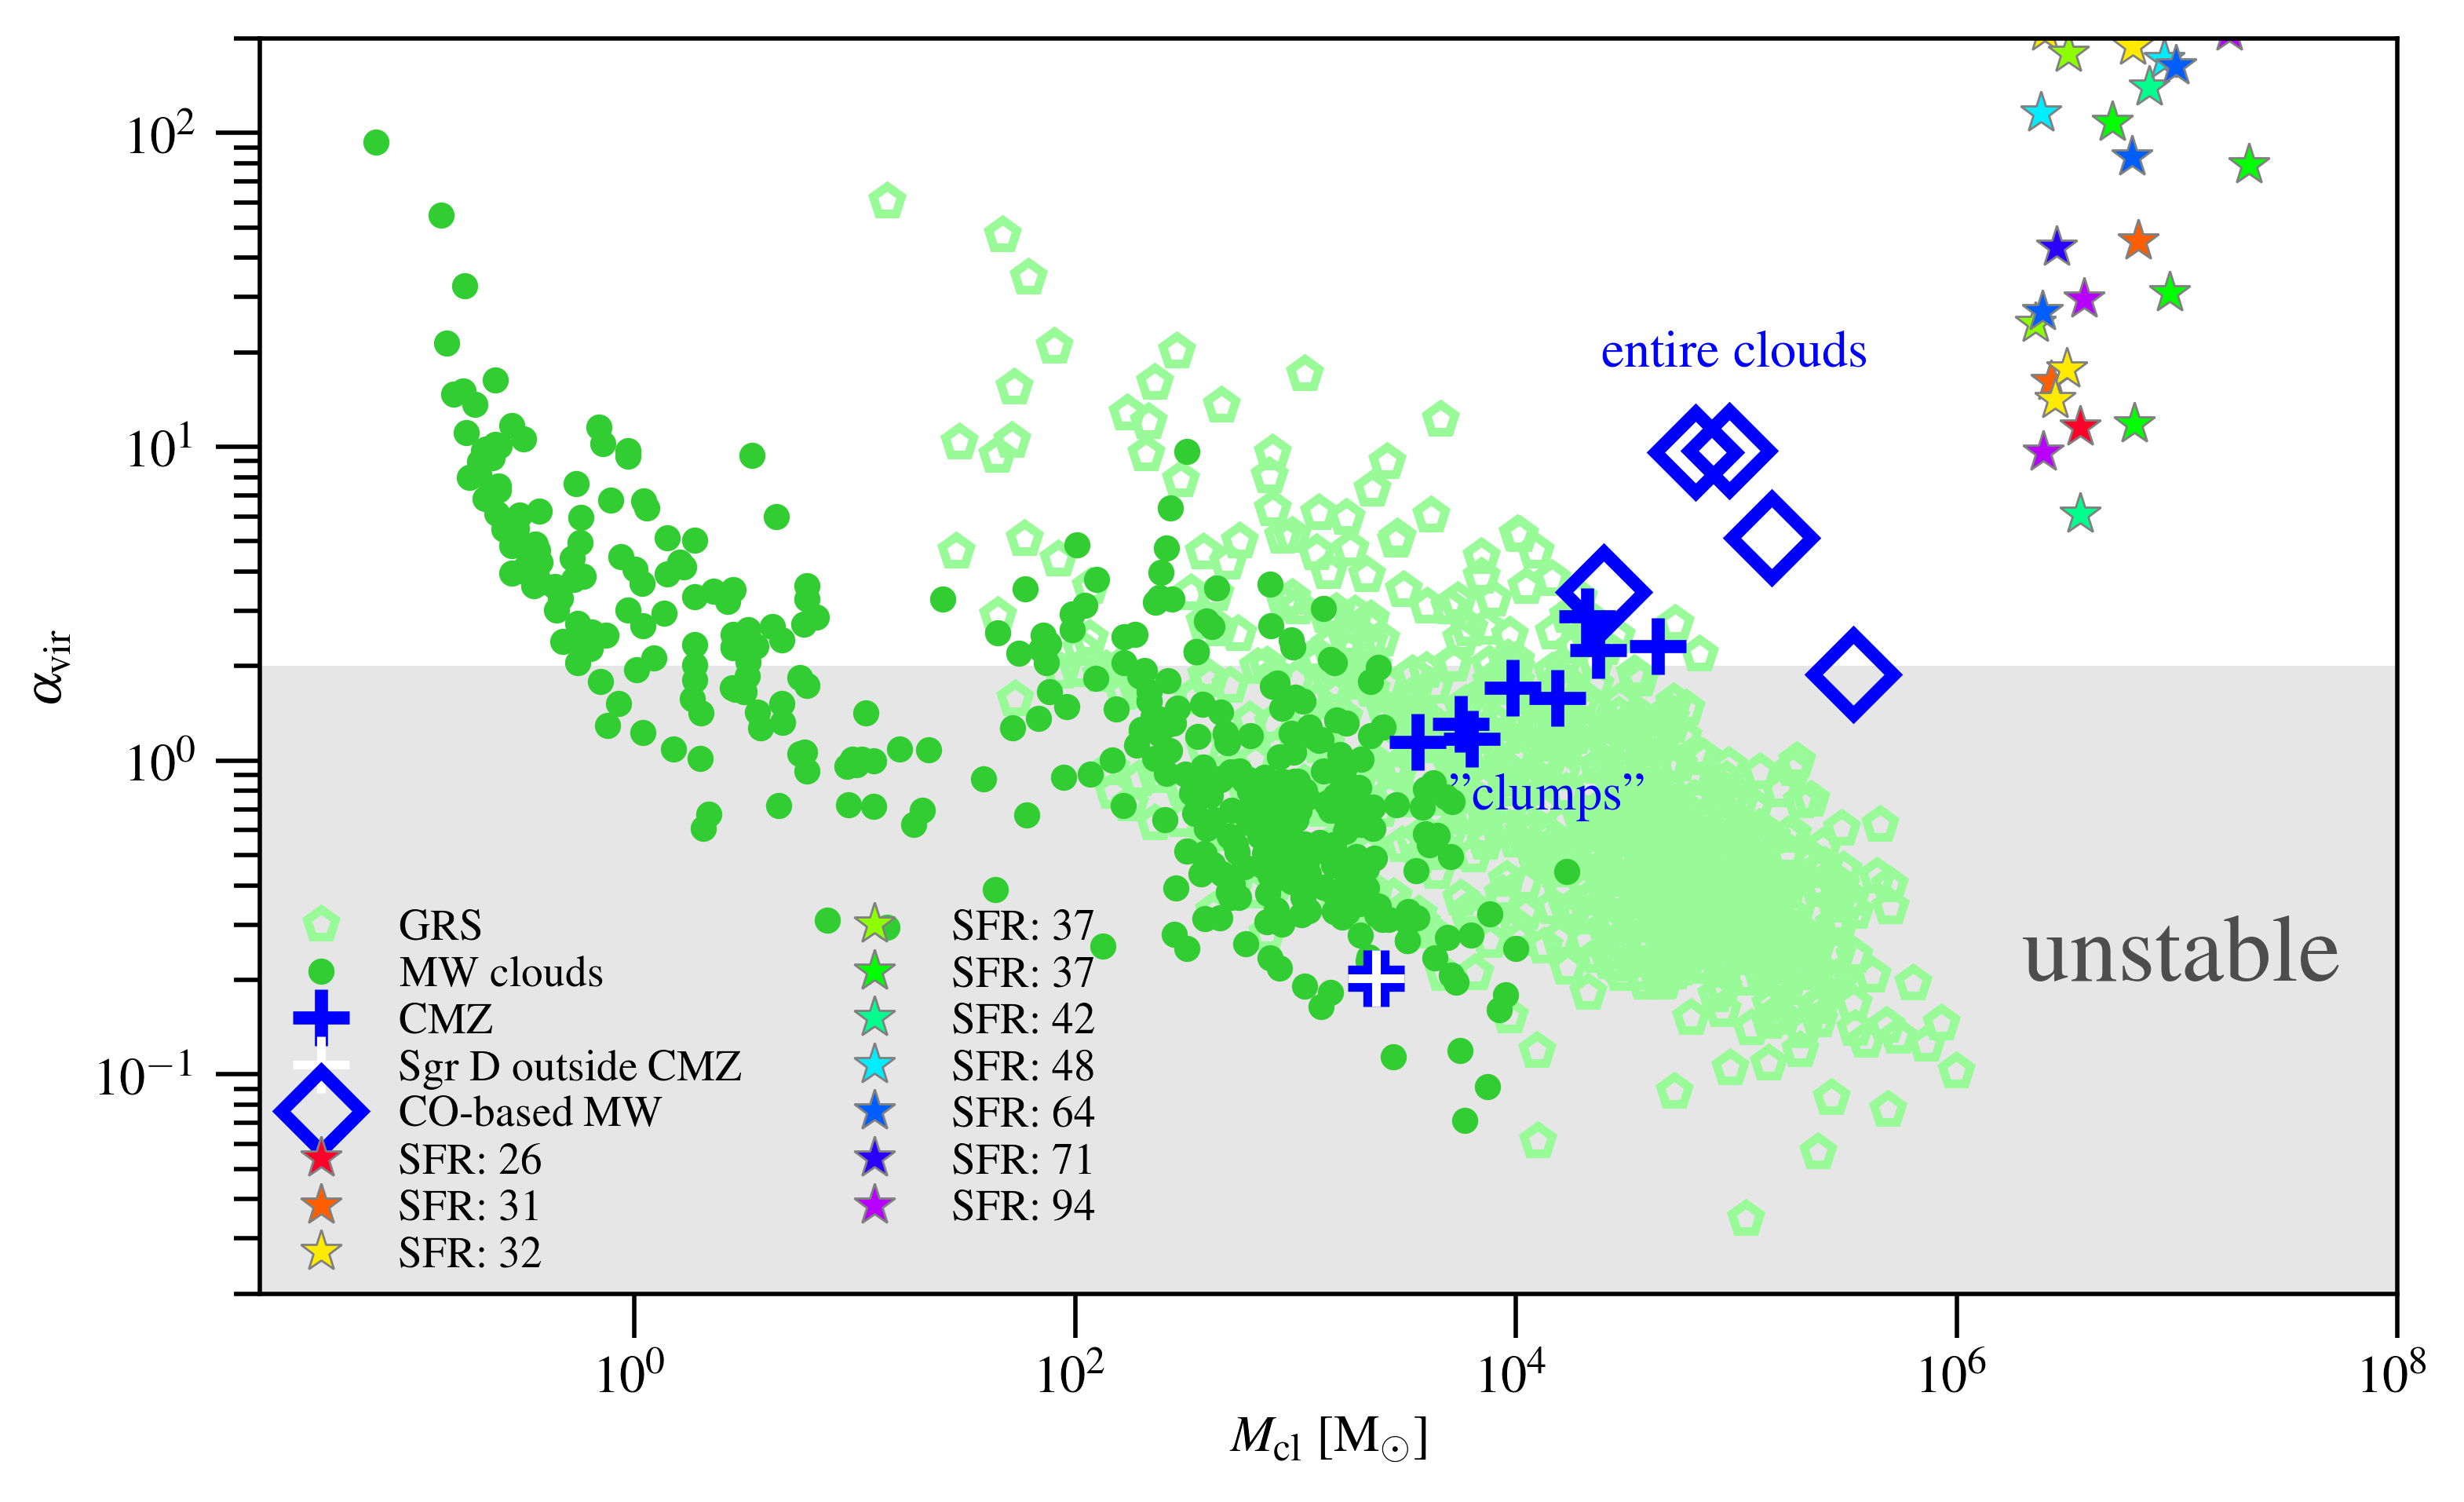
\includegraphics[trim=50 5 5 6, clip, width=0.472\textwidth]{\figpath/ss16-28-alphavir-highncut.png}
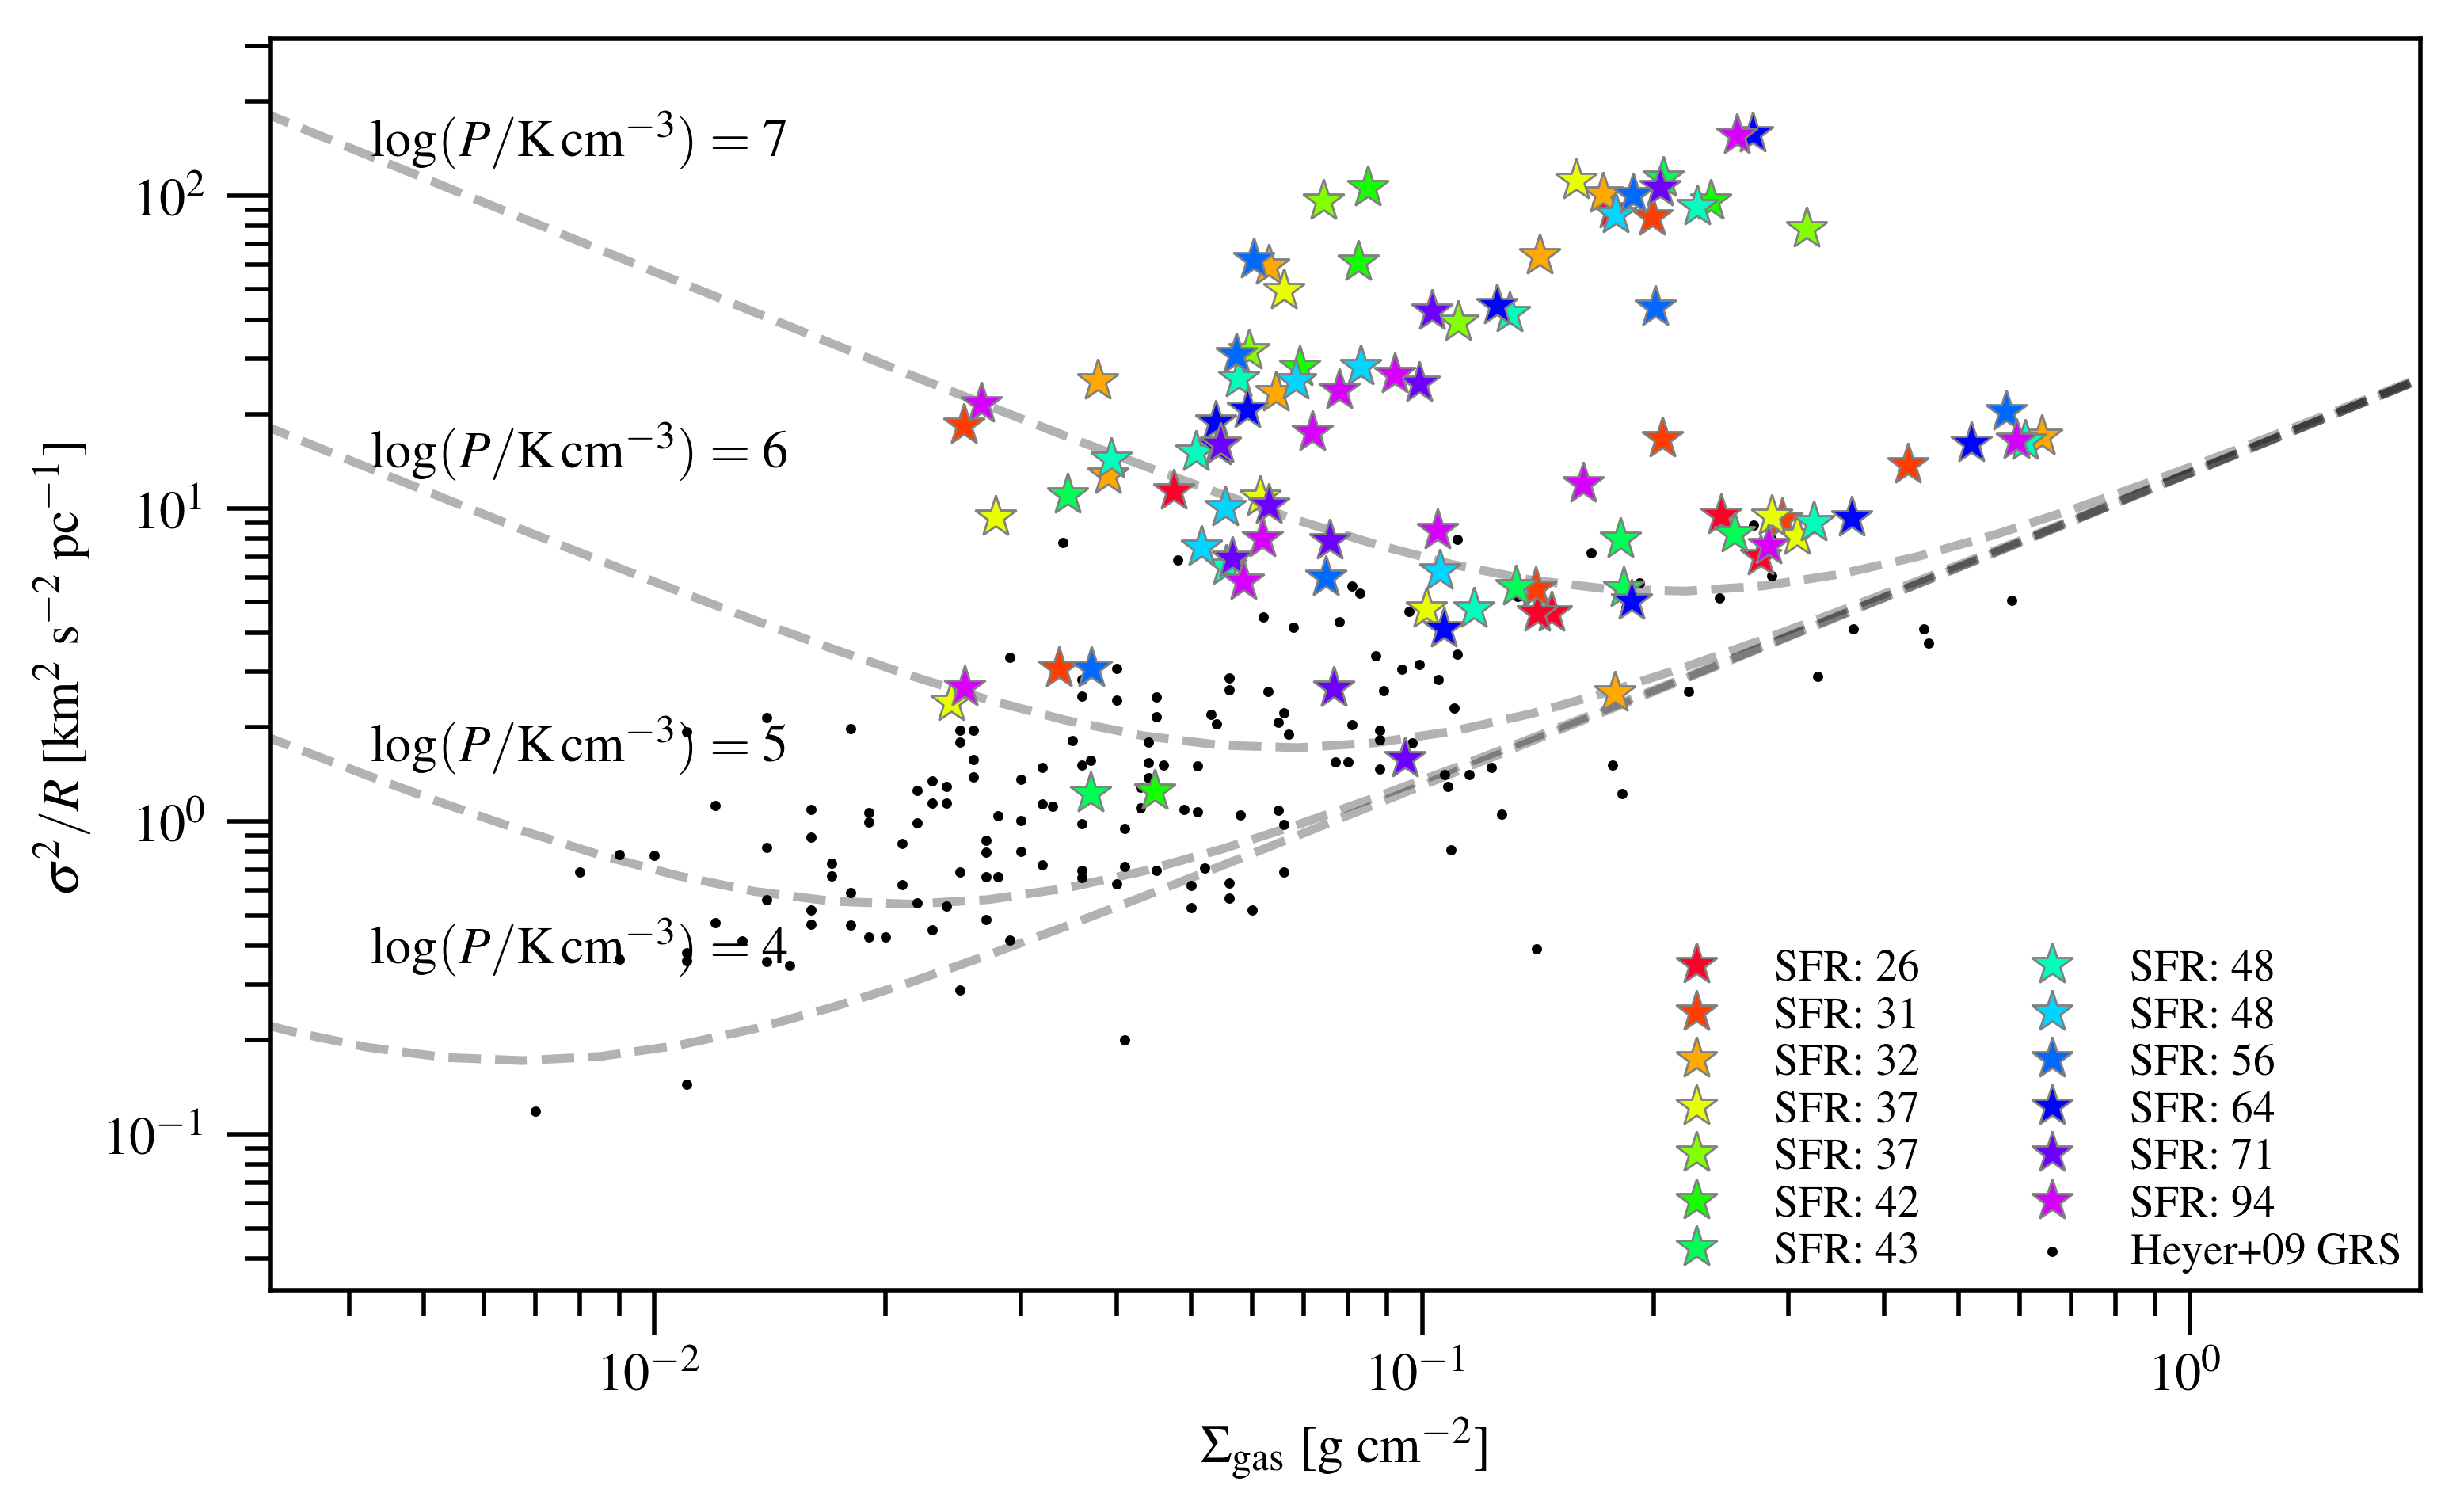
\includegraphics[trim=5 5 8 8, clip, width=0.512\textwidth]{\figpath/ss16-28_PVE.png}
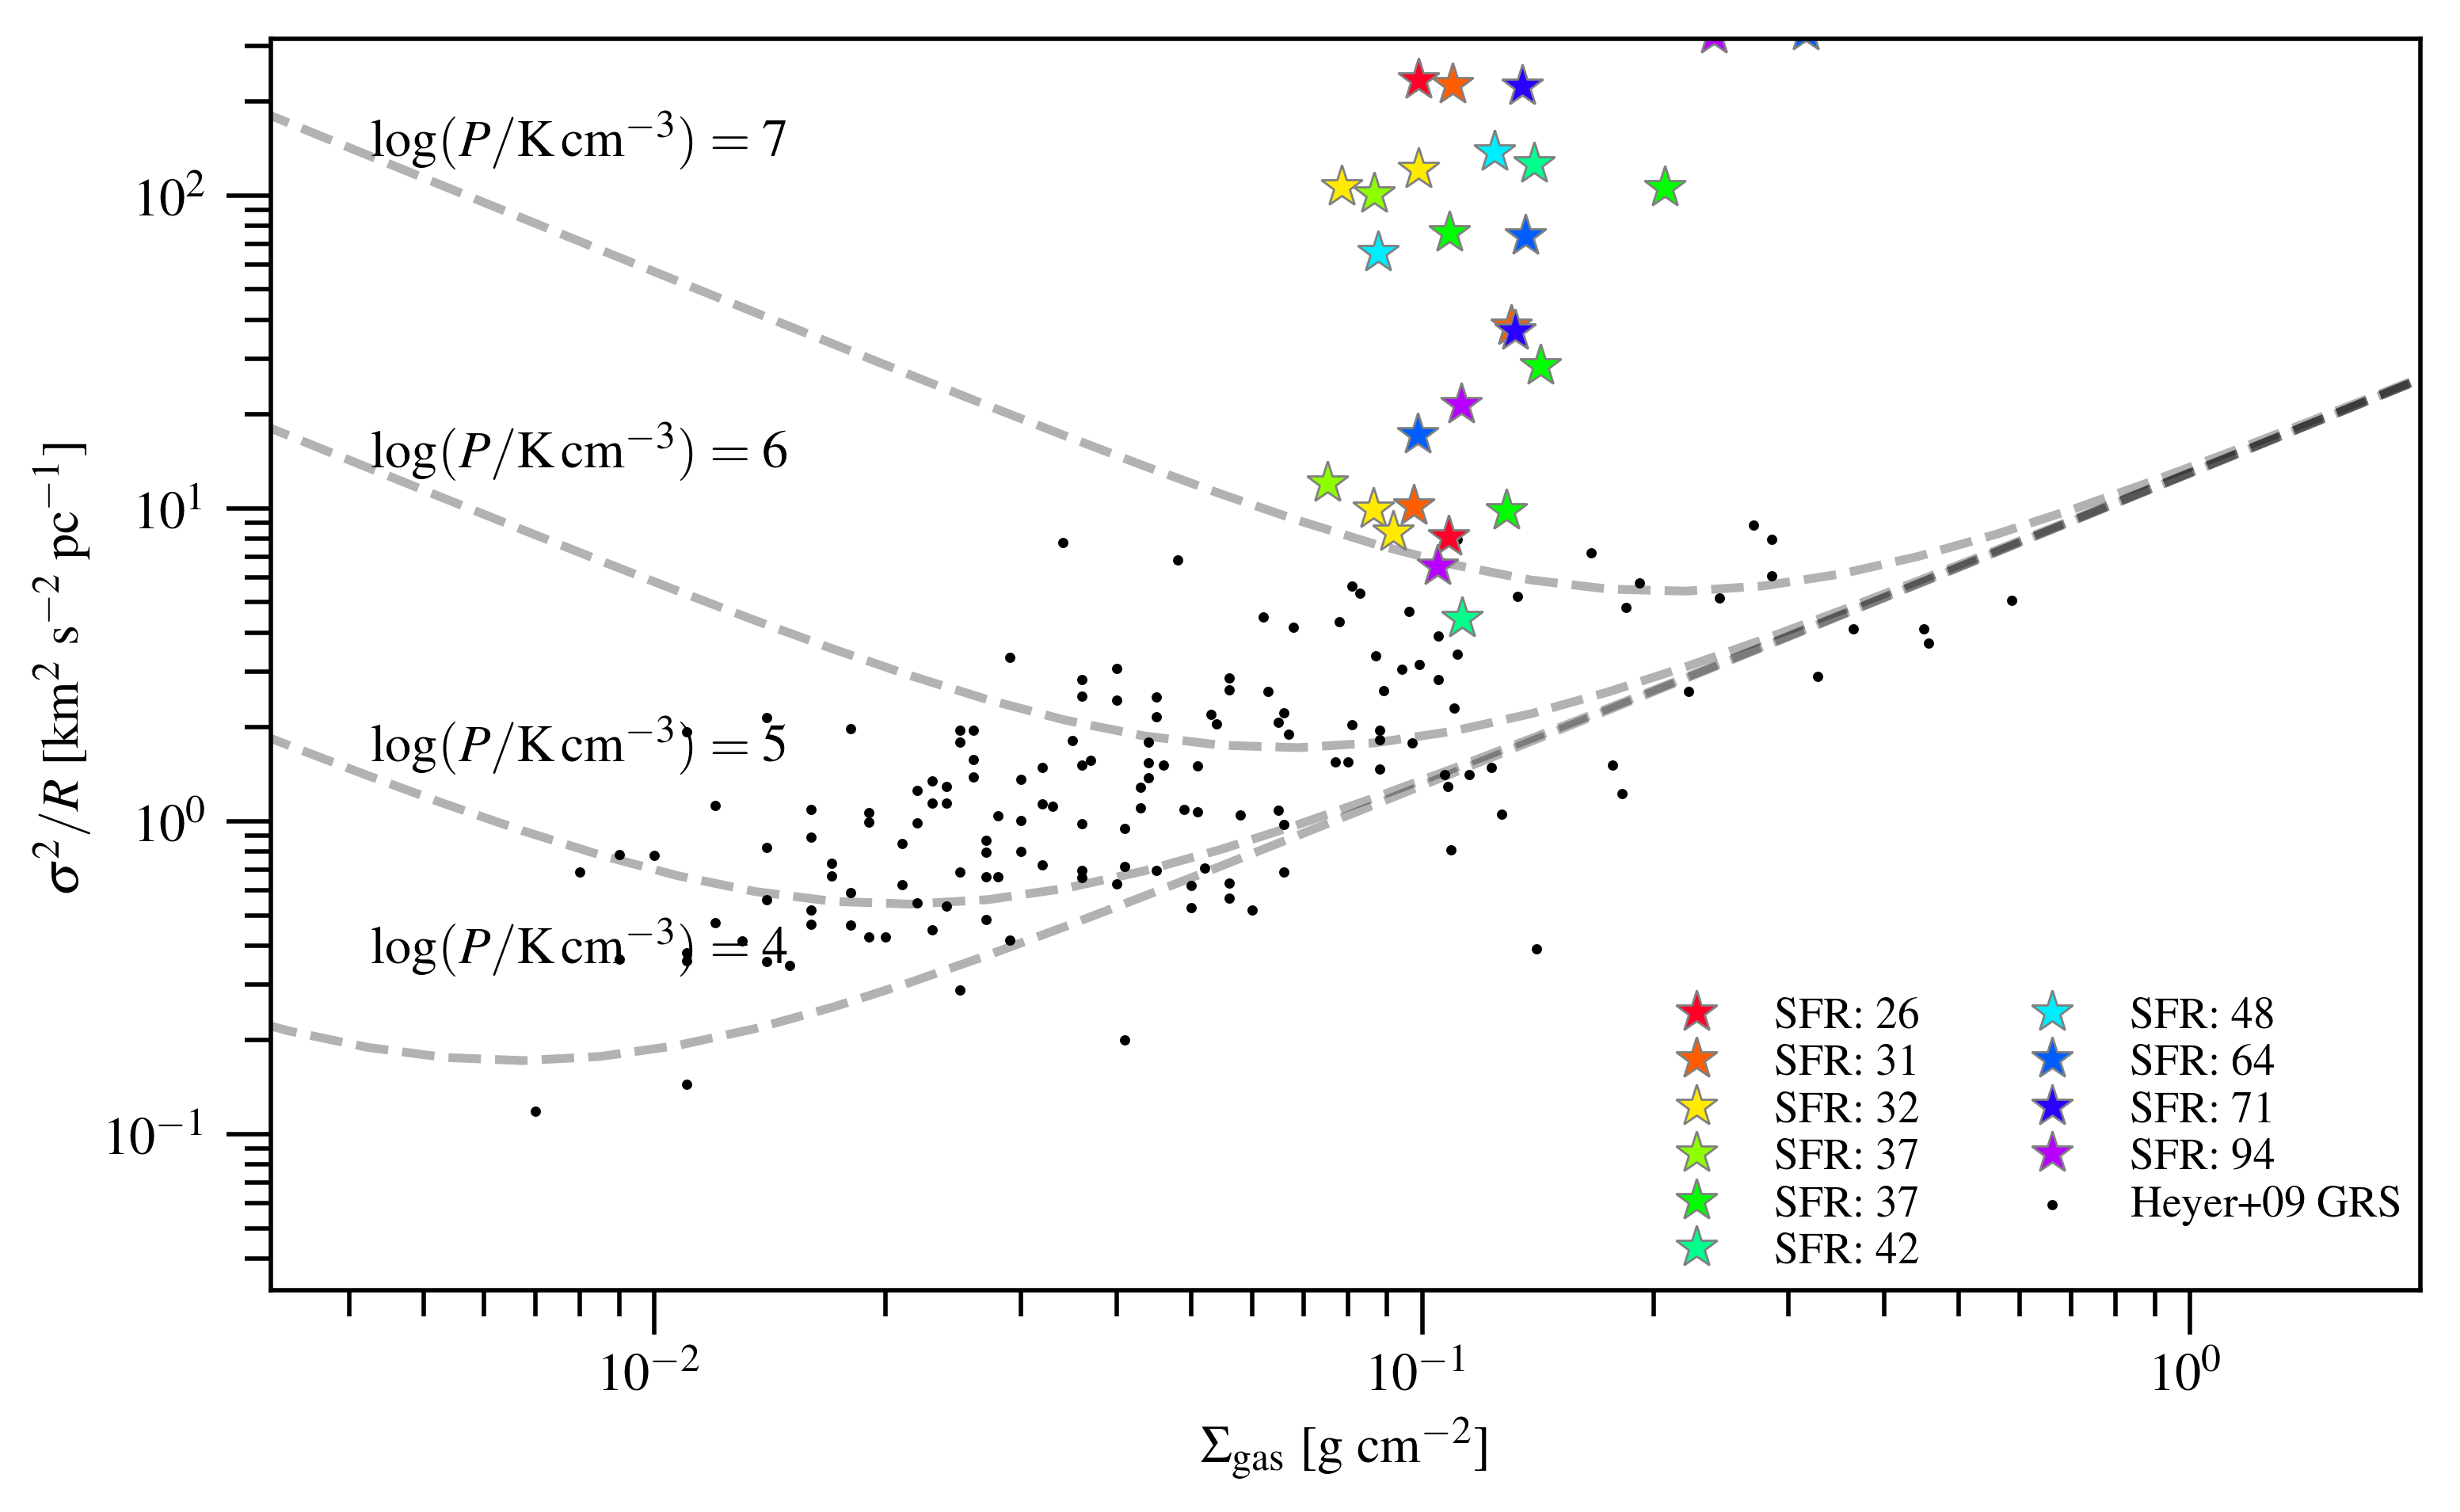
\includegraphics[trim=50 5 5 6, clip, width=0.472\textwidth]{\figpath/ss16-28-PVE-highncut.png}
\caption{
Same as \Fig{alpha16} (top panels) and \Fig{alpha27} (bottom panels), but for MCs identified across all snapshots 
(i.e., with different SFR). Star symbols are color-coded by increasing SFR.
Right panels correspond to including only the denser substructures/sub-MCs identified in \flower
(i.e., MCs here are identified with the highest $n_{\rm cut}$, see \Sec{method}).
We find no obvious differences in relation to those observed in nearby and \highz 
galaxies in the context of these cloud scaling relations.
\label{fig:alpha16-28}}
\end{figure*}




\end{document}
